\documentclass[12pt, twoside]{book}
\usepackage[a4paper, top=2.5cm, bottom=2.5cm, left=2.5cm, right=2.5cm, bindingoffset=.5cm]{geometry}
\linespread{1}
\usepackage{fancyhdr} 
\usepackage{amsmath}
\usepackage{amsthm}
\usepackage{booktabs}
\usepackage{caption}
\usepackage{subcaption}
\usepackage{amssymb}

\usepackage[english]{babel}
\usepackage[utf8]{inputenc}
%\usepackage{scrlayer-scrpage}

\usepackage{mathptmx}
\usepackage{graphicx}
\usepackage{csquotes}
\usepackage{titlesec}
\usepackage{float}
\usepackage{setspace}

\usepackage{listings}
\usepackage{lstbayes}

\usepackage{xcolor}
\usepackage{sourcecodepro}

\usepackage[T1]{fontenc}
\usepackage{array}

\usepackage{makecell}
\renewcommand\theadfont{\normalsize}
\definecolor{codegreen}{rgb}{0.0,0.5,0.0}
\definecolor{codegray}{rgb}{0.5,0.5,0.5}
\definecolor{codepurple}{rgb}{0.58,0,0.82}
\definecolor{backcolour}{rgb}{0.95,0.95,0.92}

\definecolor{backcolour2}{rgb}{0.99,0.97,0.95}
\usepackage{courier}
\definecolor{mygreen}{rgb}{0,0.6,0}
\definecolor{mygray}{rgb}{0.5,0.5,0.5}
\definecolor{mymauve}{rgb}{0.6,0.1,0.95}

\lstdefinestyle{mystyle}{
    backgroundcolor=\color{backcolour2},
    commentstyle=\color{codegreen},
    keywordstyle=\color{mymauve},
    numberstyle=\tiny\color{codegray},
    stringstyle=\color{codegreen},
    basicstyle=\ttfamily\footnotesize,
    breakatwhitespace=false,
    breaklines=true,
    captionpos=b,
    keepspaces=true,
    numbers=left,
    numbersep=5pt,
    showspaces=false,
    showstringspaces=false,
    showtabs=false,
    tabsize=2,
    literate={~} {$\sim$}{1}
}
\lstset{style=mystyle}

%\titleformat{\chapter}[block]
%  {\normalfont\LARGE\bfseries}{\thechapter.}{0.5em}{\LARGE}
%\titlespacing*{\chapter}{0pt}{-20pt}{25pt}




\usepackage{hyperref}
\usepackage{afterpage}
\newcommand\blankpage{%
    \null
    \thispagestyle{empty}%
    \addtocounter{page}{-1}%
    \newpage}
\setlength\parindent{0pt}
\begin{document}
\begin{titlepage}
\vspace{1cm}
\begin{figure}[H]
    \centering
    
\includegraphics[width=0.4\textwidth]{figures/logo.png}
\end{figure}
\begin{center}
    {\Large{Dipartimento di Fisica}}\\
    \vspace{0.3cm}
    {\Large{Corso di Laurea Magistrale}}
\end{center}
\vspace{1cm}

\begin{center}
    {\Huge {Bayesian data analysis tools for the Holmes neutrino mass experiment}}
\end{center}

\vspace{2cm}

\begin{minipage}[t]{0.47\textwidth}\raggedright
	{\large{Supervisor:\\ \bf Angelo Enrico Lodovico Nucciotti}}
    \vspace{0.5cm}
    {\large{\\Co-Supervisor:\\\bf  Matteo Borghesi}}
\end{minipage}\hfill
\begin{minipage}[t]{0.47\textwidth}\raggedleft
	{\large{Candidate: \\ \bf Pietro Campana}}
    \vspace{0.5cm}
	{\large{ \\ Id Number: \\ \bf 839735 }}
\end{minipage}

\vspace{35mm}

\centering{\large{\bf ACADEMIC YEAR 2022/2023 }}
\end{titlepage}

\begin{spacing}{1}
\pagenumbering{gobble}
\afterpage{\blankpage}

\chapter*{Abstract}
Measuring the absolute neutrino mass scale is one of the most challenging experimental endeavors in contemporary physics. Although neutrino flavor oscillations prove that at least two neutrinos have a non-zero mass, directly determining their extremely small values still requires advancing current detector technologies and performance. Model-independent methods for this measurement rely on energy and momentum conservation, analyzing the energy spectrum of beta decay or electron capture isotopes. The Holmes experiment, under development since 2014 at the cryogenic laboratory of the University of Milano-Bicocca, aims to provide a calorimetric measurement of the electron neutrino mass by studying the electron capture decay of \(^{163}\)Ho. In a calorimetric experiment, the radioactive isotope is embedded in an absorber connected to a very sensitive thermometer, measuring all the energy of the decay except for that carried away by the neutrino. The shape of the resulting calorimetric energy spectrum near the endpoint depends on the value of the electron neutrino mass.

This work outlines the development of Bayesian data analysis routines for the Holmes experiment using Stan, a specialized Hamiltonian Monte Carlo toolkit and probabilistic programming language. The primary objective is to design and fit statistical models to characterize the calorimetric spectrum of \(^{163}\)Ho and estimate the neutrino mass from its endpoint. In parallel with the software development, I have taken part in the experimental activities of the group, from the hardware setup to the first measurement campaign involving detectors implanted with \(^{163}\)Ho.

To accumulate the required statistics while maintaining an excellent energy resolution and detector time response,
Holmes uses arrays of microcalorimeters based on Transition Edge Sensors (TES). Each detector in the array consists of a
TES connected to a gold absorber implanted with \(^{163}\)Ho. The first chapter details the physical principles behind
these detectors and how the TESs in an array can be read simultaneously using Microwave Multiplexing techniques. The chapter concludes with a description of the current experimental setup.

Chapter 2 provides an introduction to Bayesian data analysis. Bayesian statistics offer a powerful framework for the estimation of uncertainty, describing unknown quantities such as the parameters of a model with probability distributions. In the Bayesian paradigm, inference is carried out by using the observed data to update the initial knowledge about a parameter, which is represented by a prior distribution, obtaining what is known as the posterior distribution. This approach offers many advantages, allowing to intuitively integrate previous knowledge about relevant quantities into the data analysis, account for various systematic effects, and constrain the parameters to their physical values. All of these features are especially useful when dealing with a limited amount of data, as is the case for most neutrino experiments. A fully Bayesian treatment of complex problems is computationally expensive, since it requires to compute integrals of distributions over many dimensions. Because of this, algorithms such as Hamiltonian Monte Carlo (HMC), a variation of Markov Chain Monte Carlo, are employed to efficiently approximate these integrals by generating samples from the target distribution. The chapter describes several useful techniques for constructing and fitting statistical models using HMC. It also covers methods for testing the proper functioning of the algorithm, evaluating goodness of fit, and comparing different models. The theoretical descriptions of these methods are complemented by practical examples of their implementation in Stan.

Leveraging these tools, the last chapter presents some applications of Bayesian data analysis tailored to the Holmes experiment. At the first order, the calorimetric spectrum of \(^{163}\)Ho consists of several Lorenzian-shaped peaks. The first part of the data analysis focuses on characterizing the peak closer to the endpoint. The main objectives at this stage are estimating the position of the peaks, assessing the influence of systematics in the energy calibration of the detectors and studying asymmetries in the lineshape due to higher order processes. The second part aims to estimate the expected sensitivity of Holmes to the neutrino mass in the near future, considering a simulated measurement with 64 detectors implanted with 1 Bq of \(^{163}\)Ho each. This section focuses on studying the influence of priors and systematics on the obtained mass upper limit and how to provide a robust expected limit from simulated data. Another central and final aspect of this analysis is how to combine data from many detectors with different characteristics, such as energy resolution and calibration systematics, in order to make inferences on a common parameter, the neutrino mass.

\tableofcontents
\end{spacing}
%\addcontentsline{toc}{chapter}{Introduction}
\thispagestyle{empty}
\pagenumbering{arabic}
%\chapter*{Introduction}

The Standard Model of particle physics predicts the existence of left-handed neutrinos, which are part of
electroweak doublets alongside charged leptons. Neutrinos are unique in that they carry zero electric charge and lack
color charge, only interacting through the weak force. Notably, the Standard Model does not include right-handed neutrino components, which leads to the prediction that their left-handed counterparts should be massless.
Neutrinos come in three distinct flavors, associated with the electron, muon, and tau charged leptons in their
respective doublets. These flavor neutrinos can be observed when they are produced alongside or from specific charged
leptons, and can be identified with the interaction states.

A groundbreaking discovery in neutrino physics came in 1998 when the Super-Kamiokande collaboration and later the SNO
collaboration in 2001 confirmed the existence of neutrino flavor oscillations. This phenomenon consists in the fact that
as neutrinos propagate over varying distances and energies, their flavor can periodically change. Its discovery established that neutrinos do indeed possess mass, and their lepton flavors can mix.
Unlike heavy charged leptons and quarks, which quickly decay or hadronize, neutrinos 
can traverse long distances. This property allows to observe neutrino flavor oscillations, which are a
consequence not only of finite masses but also of a difference between the three mass eigenstates $\nu_{1,2,3}$ and the
flavor states $\nu_{e,\mu,\tau}$. 
The mixing between these states is described by a non-trivial Pontecorvo-Maki-Nakagawa-Sakata (PMNS) matrix, akin to the
Cabibbo-Kobayashi-Maskawa (CKM) matrix in the quark sector. The PMNS matrix can be parameterized in terms of three
mixing angles, denoted as $\theta_{ij}$, and one CP-violating phase $\delta_{CP}$:
\begin{equation}
U_{PMNS} = \begin{pmatrix}
1 & 0 & 0 \\
0 & c_{23} & s_{23} \\
0 & -s_{23} & c_{23}
\end{pmatrix}
\begin{pmatrix}
c_{13} & 0 & s_{13}e^{-i\delta_{CP}} \\
0 & 1 & 0 \\
-s_{13}e^{i\delta_{CP}} & 0 & c_{13}
\end{pmatrix}
\begin{pmatrix}
c_{12} & s_{12} & 0 \\
-s_{12} & c_{12} & 0 \\
0 & 0 & 1
\end{pmatrix},
\end{equation}

Where $c_{ij} = \cos\theta_{ij}$ and $s_{ij} = \sin\theta_{ij}$. Additionally, if neutrinos are their own antiparticles,
a property denoted as being a Majorana fermion, two more phases may exist, but they cannot be measured through
oscillation experiments. For a neutrino created in a flavor state $\alpha$, the probability $P(\nu_\alpha \rightarrow
\nu_\beta)$ of detecting it in a flavor state $\beta$ after traveling through vacuum is described by the following equation:

\begin{eqnarray}
      P({\nu_\alpha \rightarrow\nu_\beta}) = \delta_{\alpha\beta} - 4\sum_{j > i}\mathrm{Re}\left(U_{\alpha j}^*\,U_{\beta j}\,
      U_{\alpha i}\,U_{\beta i}^*\right)\sin^2\left(\frac{\Delta m^2_{ji}\,L}{4E}\right) \\ 
      + 2\sum_{j > i}\mathrm{Im}
      \left(U_{\alpha j}^*\,U_{\beta j}\,U_{\alpha i}\,U_{\beta i}^*\right)\sin\left(\frac{\Delta m^2_{ji}\,L}{2E}
      \right) \nonumber
\end{eqnarray}
Here, $E$ is the neutrino energy, $L$ is the source-detector distance, and $\Delta m^2_{ji} = m_j^2 - m_i^2$. The
second term is responsible for CP violation and is present only if $\delta_{CP}\neq 0$.

Neutrino oscillations are studied using both terrestrial and astrophysical sources, and the accessible
oscillation channels depend on the energy spectrum of the neutrinos. For instance, oscillations primarily due to the
$\theta_{23}$ angle were first observed in atmospheric neutrinos, produced in
cosmic-ray interactions in the Earth's atmosphere. On the other hand, solar neutrinos, generated in the core of the Sun through fusion processes, have been crucial for
constraining $\theta_{12}$ and $\Delta m^2_{21}$. 
Because of this, the mixing angles $\theta_{23}$ and $\theta_{12}$ and the corresponding square mass differences are
commonly referred to as describing atmospheric and solar neutrino oscillations, respectively. The remaining relatively small mixing angle $\theta_{13}$ approximately decouples atmospheric and solar oscillations. 
Reactor neutrinos, produced in the cores of nuclear reactors, have provided precise measurements of $\theta_{13}$,
$\theta_{12}$, and $|\Delta m^2_{31}|$. Finally, accelerator neutrino beams have been employed to constrain various mixing
parameters, depending on the selected beam. Global analyses combining data from various sources have
been used to determine the values of all mixing angles and $\Delta m^2_{21}$, while the CP-violating phase $\delta_{CP}$ and the sign of $\Delta m^2_{31}$ remain undetermined.
This unknown sign means that there are two pssible ways to order the mass states, a problem that is known as the
neutrino mass hierarchy problem. 
In the first configuration, known as the Normal Ordering (NO), the two lightest neutrino mass
eigenstates exhibit a minimal mass difference, approximately on the order of 10 meV, while the third eigenstate
possesses a mass roughly 50 meV higher. In the Inverted Ordering (IO), the lightest neutrino mass eigenstate is
succeeded by a doublet of higher mass eigenstates, with a small mass difference within the doublet. Current experimental
data exhibit a slight preference for the Normal Ordering.


The masses of neutrinos are remarkably smaller, at least five orders of magnitude, than those of any other fermions in
the Standard Model. This significant disparity hints at the possibility of a distinct mechanism responsible for
generating them. Due to oscillations only depending on the difference between neutrino masses, their observation can only provide a lower
bound on the absolute neutrino mass scale. A direct measurement of this parameter may not only shed light on many open problems,
such as the question of mass hierarchy, but also offer new insights into the fundamental question of how these particles acquire
mass. Moreover, neutrinos play a pivotal role in shaping the evolution of the cosmos on
a large scale, and a direct measurement of the neutrino mass could thus serve as a crucial input for models describing the formation of cosmological structures.


\pagestyle{fancy}
\renewcommand{\sectionmark}[1]{\markboth{#1}{#1}}
\fancyhead{}
\fancyfoot{}
\fancyhead[RE]{\thesection \ --\ \leftmark}
\fancyhead[LO]{\thesection \ --\ \leftmark}
\fancyhead[RO]{\thepage}
\fancyhead[LE]{\thepage}

\setcounter{page}{0}
\chapter{Holmes}
This chapter presents the motivations, underlyig physical principles and current experimental status of the Holmes
experiment. The first section briefly reviews the discovery of nonzero neutrtino masses and its implications, before
presenting the various experiments currently trying to measure the electronic neutrino mass and describing the decay of
$^{163}$Ho, the isotope used by Holmes. The second section details the microcalorimeter detectors employed in the experiment,
which consist of arrays of Transition Edge Sensors that are readout with a Microwave Multiplexing technique. The chapter concludes with a
description of the experimental setup used in the first measurement campaign of Holmes.
\section{The neutrino mass}
\subsection{Neutrino physics and oscillations}

The Standard Model of particle physics predicts the existence of left-handed neutrinos, which are part of
electroweak doublets alongside charged leptons. Neutrinos are unique in that they carry zero electric charge and lack
color charge, only interacting through the weak force. Notably, the Standard Model does not include right-handed neutrino components, which leads to the prediction that their left-handed counterparts should be massless.
Neutrinos come in three distinct flavors, associated with the electron, muon, and tau charged leptons in their
respective doublets. These flavor neutrinos can be observed when they are produced alongside or from specific charged
leptons, and can be identified with the interaction states.

A groundbreaking discovery in neutrino physics came in 1998 when the Super-Kamiokande collaboration  \cite{fukuda1998evidence} and later the SNO
collaboration in 2001  \cite{ahmad2001measurement} confirmed the existence of neutrino flavor oscillations. This phenomenon consists in the fact that
as neutrinos propagate over varying distances and energies, their flavor can periodically change. Its discovery established that neutrinos do indeed possess mass, and their lepton flavors can mix.
Unlike heavy charged leptons and quarks, which quickly decay or hadronize, neutrinos 
can traverse long distances. This property allows observing neutrino flavor oscillations, which are a
consequence not only of finite masses but also of a difference between the three mass eigenstates $\nu_{1,2,3}$ and the
flavor states $\nu_{e,\mu,\tau}$. 
The mixing between these states is described by a non-trivial Pontecorvo-Maki-Nakagawa-Sakata (PMNS) matrix, akin to the
Cabibbo-Kobayashi-Maskawa (CKM) matrix in the quark sector. The PMNS matrix can be parameterized in terms of three
mixing angles, denoted as $\theta_{ij}$, and one CP-violating phase $\delta_{CP}$:
\begin{equation}
U_{PMNS} = \begin{pmatrix}
1 & 0 & 0 \\
0 & c_{23} & s_{23} \\
0 & -s_{23} & c_{23}
\end{pmatrix}
\begin{pmatrix}
c_{13} & 0 & s_{13}e^{-i\delta_{CP}} \\
0 & 1 & 0 \\
-s_{13}e^{i\delta_{CP}} & 0 & c_{13}
\end{pmatrix}
\begin{pmatrix}
c_{12} & s_{12} & 0 \\
-s_{12} & c_{12} & 0 \\
0 & 0 & 1
\end{pmatrix},
\end{equation}

Where $c_{ij} = \cos\theta_{ij}$ and $s_{ij} = \sin\theta_{ij}$. Additionally, if neutrinos are their own antiparticles,
a property denoted as being a Majorana fermion, two more phases may exist, but they cannot be measured through
oscillation experiments. For a neutrino created in a flavor state $\alpha$, the probability $P(\nu_\alpha \rightarrow
\nu_\beta)$ of detecting it in a flavor state $\beta$ after traveling through vacuum is described by the following equation:

\begin{eqnarray}
      P({\nu_\alpha \rightarrow\nu_\beta}) = \delta_{\alpha\beta} - 4\sum_{j > i}\mathrm{Re}\left(U_{\alpha j}^*\,U_{\beta j}\,
      U_{\alpha i}\,U_{\beta i}^*\right)\sin^2\left(\frac{\Delta m^2_{ji}\,L}{4E}\right) \\ 
      + 2\sum_{j > i}\mathrm{Im}
      \left(U_{\alpha j}^*\,U_{\beta j}\,U_{\alpha i}\,U_{\beta i}^*\right)\sin\left(\frac{\Delta m^2_{ji}\,L}{2E}
      \right) \nonumber
\end{eqnarray}
Here, $E$ is the neutrino energy, $L$ is the source-detector distance, and $\Delta m^2_{ji} = m_j^2 - m_i^2$. The
second term is responsible for CP violation and is present only if $\delta_{CP}\neq 0$.

Neutrino oscillations are studied using both terrestrial and astrophysical sources, and the accessible
oscillation channels depend on the energy spectrum of the neutrinos. For instance, oscillations primarily due to the
$\theta_{23}$ angle were first observed in atmospheric neutrinos, produced in
cosmic-ray interactions in the Earth's atmosphere. On the other hand, solar neutrinos, generated in the core of the Sun through fusion processes, have been crucial for
constraining $\theta_{12}$ and $\Delta m^2_{21}$. 
Because of this, the mixing angles $\theta_{23}$ and $\theta_{12}$ and the corresponding square mass differences are
commonly referred to as describing atmospheric and solar neutrino oscillations, respectively. The remaining relatively small mixing angle $\theta_{13}$ approximately decouples atmospheric and solar oscillations. 
Reactor neutrinos, produced in the cores of nuclear reactors, have provided precise measurements of $\theta_{13}$,
$\theta_{12}$, and $|\Delta m^2_{31}|$. Finally, accelerator neutrino beams have been employed to constrain various mixing
parameters, depending on the selected beam. Global analyses combining data from various sources have
been used to determine the values of all mixing angles and $\Delta m^2_{21}$, while the CP-violating phase $\delta_{CP}
$ and the sign of $\Delta m^2_{31}$ remain undetermined \cite{esteban2020fate}.
This unknown sign means that there are two possible ways to order the mass states, a problem that is known as the
neutrino mass hierarchy problem. 
In the first configuration, known as the Normal Ordering (NO), the two lightest neutrino mass
eigenstates exhibit a minimal mass difference, approximately on the order of 10 meV, while the third eigenstate
possesses a mass roughly 50 meV higher. In the Inverted Ordering (IO), the lightest neutrino mass eigenstate is
succeeded by a doublet of higher mass eigenstates, with a small mass difference within the doublet. Current experimental
data exhibit a slight preference for the Normal Ordering.


The masses of neutrinos are remarkably smaller, at least five orders of magnitude, than those of any other fermion in
the Standard Model. This significant disparity hints at the possibility of a distinct mechanism responsible for
generating them. Due to oscillations only depending on the difference between neutrino masses, their observation can only provide a lower
bound on the absolute neutrino mass scale. A direct measurement of this parameter may not only shed light on many open problems,
such as the question of mass hierarchy, but also offer new insights into the fundamental question of how these particles acquire
mass. Moreover, neutrinos play a pivotal role in shaping the evolution of the cosmos on
a large scale, and a direct measurement of the neutrino mass could thus serve as a crucial input for models describing the formation of cosmological structures.


\subsection{Direct mass measurements}
The only known model independent way to measure the absolute scale of the neutrino mass is by observing its influence on
the energy spectrum of beta and electronic capture decays, which only assumes conservation of energy and momentum.
For example, the beta decay:
\begin{equation}
 (Z, A) \rightarrow (Z + 1, A) + e^- + \bar{\nu}_e
\end{equation}
\[
 n \rightarrow p + e^- + \bar{\nu}_e
\]
is a fundamental and widely studied process in atomic physics. Being a three body decay, the energy spectrum of the
produced electron and antineutrino are continuous. Excluding the negligible recoil of the nucleus, if neutrinos had zero mass the maximum energy reacheable by the
electron would be all of the energy released in the decay, which is known as the $Q$ value. 
Finite neutrino masses sligthly reduce the maximum energy available for the electron, altering the endpoint of its
spectrum. Theoretically, since the electronic (anti)neutrino is a superposition of the three mass eigenstates, each of
them changes the spectrum in a slightly different way. However, for the current
experimental resolution and available data discerning the effect of the three netrino masses is well beyond reach.
Because of this, the decay spectrum is usually considered to be dependent only on one neutrino mass, which is denoted as
the effective electronic
(anti)neutrino mass: 
\begin{equation}
 m_{\overline{\nu}_{e}}^{2} = m_{\nu_{e}}^{2}=\sum_{i}|U_{e i}|^{2}m_{\nu_{i}}^{2}
\end{equation}
The Fermi theory then provides the energy spectrum of the electron:
\begin{equation}
  \frac{d N}{d E} \propto p(E+m_{e}c^{2})(Q-E)\sqrt{(Q-E)^{2}-m_{\overline{\nu}_{e}}^{2}c^{4}}
\end{equation}
Many experiments aiming to measure the neutrino mass use tritium $^3$H, a $\beta^-$ decay isotope with a relatively low $Q\sim
18$keV and a precisely computable nuclear matrix element. As of today, the most stringent upper limits on
$m_{\overline{\nu}_{e}}$ have been reached with spectrometric experiments, where a
high-activity source is placed outside of the detector and only the electrons with energy close to $Q$ are selected with
sophisticated filters.
However, an external source introduces a series of systematics that ultimately limit this approach, such as energy
loss, source charging, backscattering of electrons on the detector and energy dependence of detection efficiency.
Moreover, it is usually only possible to use tritium in its molecular form $^2$T instead of $^3$H, which introduces
further uncertainty due to molecular energy levels and internal motion.
\subsubsection*{Katrin}

The Katrin experiment holds the current best limit on the neutrino mass, having achieved $m_{\overline{\nu}_{e}} < 0.8$ eV at a 90\%
confidence level  \cite{katrin2022direct}. Katrin aims to attain a sensitivity of approximately 0.2 eV at 90\% CL within a total measurement time of 1,000 days.
To achieve these cutting-edge results, Katrin combines a high-activity molecular tritium source with a high-resolution
spectrometer of the magnetic adiabatic collimation and electrostatic (MAC-E)-filter type. The experiment employs a
system of superconducting magnets to guide electrons from the source to the spectrometer without altering their
energy, while differential and cryogenic pumping systems are used to reduce tritium flow. The MAC-E-filter type
spectrometer acts as an electrostatic high-pass filter, transmitting only high-energy electrons. Finally, a focal-plane
detector measures the count rate of transmitted electrons.
The second physics run of Katrin demonstrated significant improvements, including operating the tritium source at
its nominal activity and reducing background levels by 25\%. This allowed for a higher signal strength and overall higher statistics, thus improving sensitivity.

\begin{figure}[t]
  \centering
  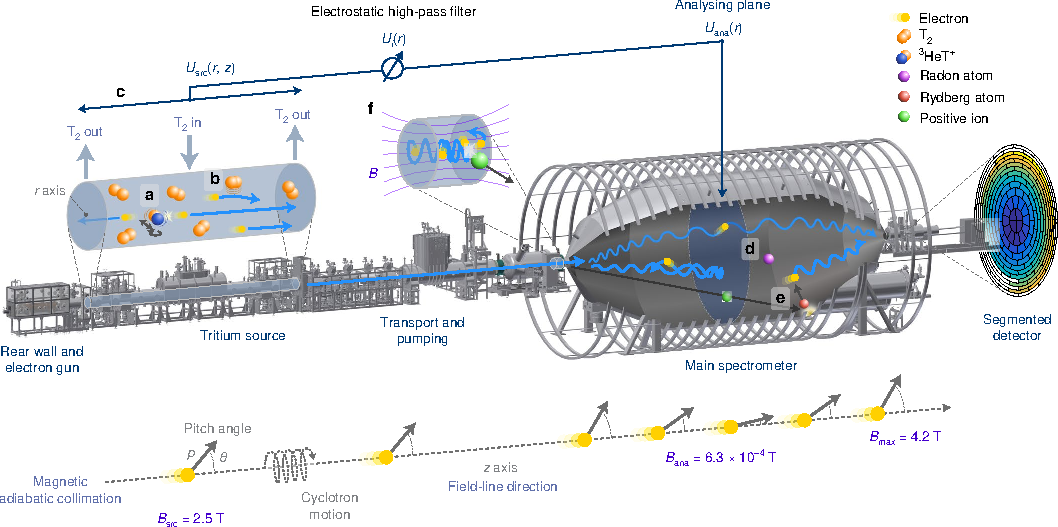
\includegraphics[width=0.92\textwidth]{figures/ch1/katrin.pdf}
  \caption{Illustration of the 70-m-long KATRIN beamline, also showing the transport of $\beta^-$ electrons and magnetic adiabatic 
collimation of their momenta in the spectrometer. View into the tritium source depicts three systematic effects:
molecular excitations during $\beta$ -decay (a), 
scattering of electrons off the gas molecules (b) and spatial distribution of the electric potential in the source (c). The view into the spectrometer 
illustrates the main background processes: radon decays (d), highly excited rydberg atoms 
due to $\alpha$-decays of $^{210}$Po (e) and positive ions created in a Penning trap between the two spectrometers 
(f). Image taken from  \cite{katrin2022direct}.}
  \label{fig:katrin}
\end{figure}
\subsubsection*{Project 8}

Traditional experiments using molecular tritium face limitations when neutrino masses approach $\sim$0.1 eV
due to broadening caused by internal molecular motion. To overcome these problems and achieve a hypotetical sensitivity
of 40 meV, the Project 8 Collaboration developed a novel technique called cyclotron radiation emission
spectroscopy (CRES) \cite{P8esfahani2017determining}. CRES utilizes the cyclotron emission from electrons or positrons
spiraling in a strong magnetic field to
determine their energies. This technique allows for incredibly precise measurements and is relatively immune to background interference, making it ideal for studying beta decay electrons.
The core of the CRES apparatus is a cryogenic gas cell, where electrons produced in radioactive decay are magnetically
trapped while emitting cyclotron radiation. The cell is placed in a superconducting magnet, generating an axial magnetic
field that confines electrons radially, while additional coils provide magnetic trap potentials to confine the electrons axially.

After demonstrating the feasibility of CRES on single electrons emitted from $^{83m}$Kr in the first phase of the experiment,
this technique was applied to perform the first spectrum measurement of molecular tritium beta decay near the
end-point region. This enabled the first neutrino mass limit using CRES, with a result of $m_{\overline{\nu}_{e}} < 155$ eV, concluding the
second phase. Moreover, the experiment achieved a stringent upper limit on backgrounds ($\le 3 \times 10^{-10}$ counts
eV$^{-1}$ s$^{-1}$) by characterizing and rejecting radiofrequency noise fluctuations, enabling a zero-background measurement. The objective of phase III is to demonstrate the ability to make CRES measurements in free space and produce and trap atomic tritium. The final phase aims to use atomic tritium to measure the neutrino mass with a sensitivity of 40 meV.
\begin{figure}[t]
\begin{subfigure}[b]{0.5\linewidth}
    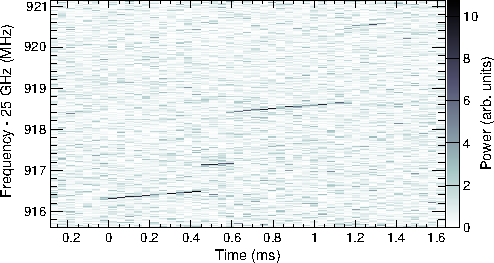
\includegraphics[width=\linewidth]{figures/ch1/p8electron.pdf}
    \caption{}
  \end{subfigure}
\hfill
\begin{subfigure}[b]{0.45\linewidth}
    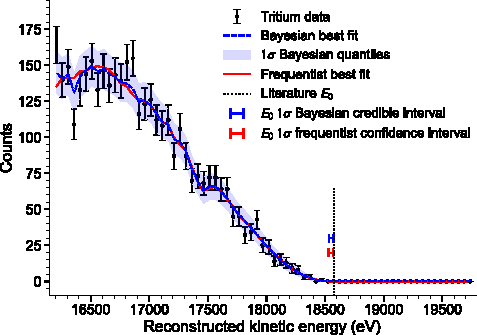
\includegraphics[width=\linewidth]{figures/ch1/p8V2.pdf}
    \caption{}
  \end{subfigure}
  \caption{Spectrogram of the first CRES event detected from a
tritium beta decay electron (a). Latest results of the project8 collaboration showing frequentist and bayesian fits of
the spectrum endpoint (b). Images taken from  \cite{P8esfahani2023tritium}. }
\label{fig:p8}
\end{figure}


\subsubsection*{Calorimetric experiments}
By embedding the radioactive source in the detector, calorimetric experiments measure all the energy of the decay,
excluding that carried away by the neutrino. This approach
minimizes the systematics due to source-related effects that are characteristic of spectrometric experiments. However, it comes
with the limitation that the entire energy spectrum is acquired, which imposes constraints on the source intensity in
order to limit the pile-up.
Pile-up events occur when multiple decays take place within a time interval shorter than the detector's time resolution
and are recorded as a single decay with summed energy.
The key component of these experiments is the microcalorimeter, a thermal detector that measures energy deposition
through heat conversion. When energy $E$ is deposited in the detector, it causes a temperature increase $\Delta T$,
which is proportional to $E/C$, where $C$ is the heat capacity of the detector. 

The thermodinamic limit defines how much
the measured energy fluctuates due to heat exchange with a thermal bath of temperature $T$:

\begin{equation}
  \Delta E \propto \sqrt{k_b T^2 C}
\end{equation}
Because of this, Low Temperature Detectors (LTDs) with small $C$ are employed in these experiments to minimize the thermal noise and achieve the best energy resolution possible.
Two completed experiments following this calorimetric approach used the beta decay of $^{187}$Re as their source. Known
as MANU and MIBETA  \cite{MANU} \cite{MIBETA}, they employed metallic and dielectric rhenium absorbers, respectively, to set limits of
$m_{\nu_{e}} < 19$ eV and $m_{\nu_{e}} < 15$ eV at the end of their measurement campaigns. However, these experiments
encountered challenges due to unexpected behaviors of metallic rhenium absorbers, including the Beta Environmental Fine
Structure (BEFS) \cite{koonin1991environmental} phenomenon, which rendered $^{187}$Re unsuitable for larger-scale experiments.

In recent years, significant interest has emerged in the use of $^{163}$Ho for estimating neutrino masses, which decays
via Electron Capture on an excited state of $^{163}$Dy. This isotope
possesses a lower $Q = 2833 \pm 30$ (stat) $\pm$ 15 (syst) eV compared to $^3$H and a shorter half-life
$T_{1/2} = 4570$ y than $^{187}$Re. 
A shorter half-life allows embedding smaller quantities of the isotope in the detectors, reducing the impact on their heat
capacity and thus preserving energy resolution.
The relatively short half-life and low Q value of $^{163}$Ho also allow for the use of a small absorbing volume, resulting in excellent energy resolution compared to other detectors in this energy range.
While other isotopes with lower Q values have been proposed, they often have extremely long half-lives, making
calorimetric experiments challenging or unfeasible in practice.

Among various proposed methods for measuring the neutrino mass with $^{163}$Ho, the calorimetric de-excitation spectrum
end-point measurement has shown to be the most promising.
Two collaborations, ECHo \cite{echofirst} and HOLMES \cite{alpert2015holmes}, are currently developing large-array experiments using Magnetic Metallic
Calorimeters (MMCs) and Transition Edge Sensors (TESs), respectively. The ECHO
collaboration has performed its first measurement campaign, reaching a limit of $m_{\nu_{e}}<150$eV at
90\% CL  \cite{velte2019high}.

In summary, a calorimetric experiment aiming for high sensitivity in neutrino mass determination has two primary
requirements: exceptional energy resolution and a substantial number of recorded events, which must be balanced with the
occurrence of pile-up events. For the Holmes experiment, Transition Edge Sensors (TESs) have been selected as the most
suitable detectors to satisfy these requirements. Their intrinsic energy resolution is exceptionally high, with resolving powers $\Delta E / E$
exceeding $10^3$ for single photons or electrons. This resolution can be preserved even when measuring arrays of
many calorimeters in a multiplexed setup, which allows accumulating the needed statistics and maintaining a fast signal
response.
\subsection{EC decay of $^{163}Ho$}

In the process of electron capture (EC) decay, an unstable nucleus captures an atomic electron, resulting in the production of a neutron, the emission of a neutrino, and the release of internal bremsstrahlung radiation. This process also leaves the daughter atom in an excited state, and subsequent emissions of X-rays and Auger electrons occur as the electron shell's vacancy is filled. In cases where the nuclide remains in an excited energy state, gamma radiation may be emitted. 

The EC decay of $^{163}$Ho can be represented as:


\begin{figure}[t]
  \begin{minipage}{0.43\linewidth}
    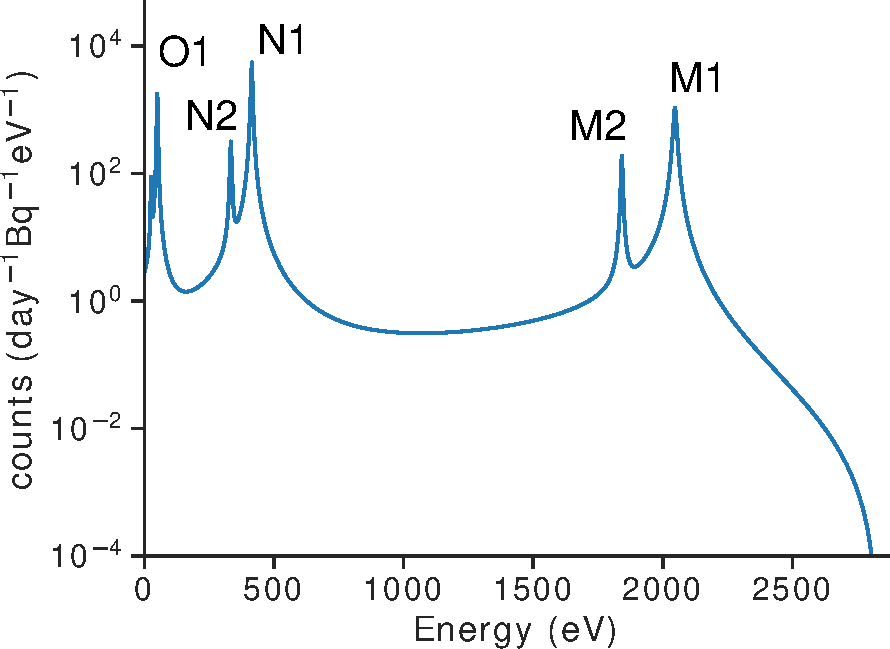
\includegraphics[width=\linewidth]{figures/ch1/Ho.pdf}
  \end{minipage}
  \hfill
  \begin{minipage}{0.58\linewidth}
      \centering
      \begin{tabular}{|c|c|c|c|c|}
        \hline
        Name & Orbital & \(E_H\) (eV) & \(\Gamma_H\) (eV) & $I_H$ \\
        \hline
        M1 & 3s & 2047 & 13.2 & 1 \\
        M2 & 3p$_{1 / 2}$ & 1842 & 6.0 & 0.0526 \\
        N1 & 4s & 414.2 & 5.4 & 0.2329 \\
        N2 & 4p & 333.5 & 5.3 & 0.0119 \\
        O1 & 5s & 49.9 & 3.0 & 0.0345 \\
        O2 & 5p$_{1 / 2}$ & 26.3 & 3.0 & 0.0015 \\
        \hline
    \end{tabular}
  \end{minipage}
\caption{first-order calorimetric spectrum of the $^{163}$Ho electronic capture decay, with $Q=2833$eV. The table shows
the names, corresponding electronic orbitals and parameters of the Lorentzian peaks.}
\label{fig:Hofirstorder}
\end{figure}
\begin{equation}
  ^{163}\text{Ho} + e^- \rightarrow ^{163}\text{Dy}_H + \nu_e \rightarrow ^{163}\text{Dy} + E_c
\end{equation}
Where $H$ labels the shell from which the electron has been captured, and $E_c$ represents all the energy of the decay
measured in a calorimetric experiment, which only excludes that of the neutrino. In the specific case of the EC decay of $^{163}
$Ho, there is no gamma emission, and the Dy atoms primarily decay through Auger processes rather
than X-rays. Therefore:
\begin{equation}
  E_c = \text{nuclear recoil} + \text{inner bremsstrahlung} + \text{Auger electrons} + \text{X-rays}
\end{equation}
Unlike beta decay, in EC decay the energy spectrum of the resulting neutrinos is similar to that of a two-body decay,
with the neutrino having an energy approximately equal to \(Q - E_H\), where \(E_H\) represents the binding energy of an
electronic
shell. The
complex structure of $^{163}$Ho poses challenges in predicting the shape of the calorimetric EC spectrum, and a
comprehensive description of its features still requries to be validated with extensive experimental data. At the first-order, the calorimetric spectrum consists of several Lorentzian-shaped peaks with energy \(E_H\) and natural width \(\Gamma_H\):

\begin{equation}\label{eq:hofirstorder}
\frac{dN_{EC}}{dE_c} \propto (Q - E_c)\sqrt{(Q - E_c)^2 - m_{\nu_e}^2}
\sum_H I_H\frac{\Gamma_H/2\pi}{(E_c - E_H)^2 + \Gamma_H^2/4}
\end{equation}

In this equation, \(I_H=|\phi_H(0)|^2 n_H B_{H}\) represents the intensity of each peak, where \(\phi(0)\) is the
wavefunction of the captured electron at the origin, \(n_H\) is the electron occupancy, and \(B_H\) is a corrective
factor accounting for atomic overlap and exchange. For $^{163}$Ho, the first-order spectrum consists of six main
Breit-Wigner peaks (M1, M2, N1, N2, O1 and O2). Their predicted parameters and the spectrum are shown in Fig
\ref{fig:Hofirstorder}.
As with beta decay, the endpoint region is the most sensitive to the neutrino mass, and the true energy spectrum should be
a coherent sum of three spectra with different endpoints corresponding to the three neutrino mass states, reducing to a
single spectrum with endpoint $Q-m_{\nu_{e}}$ if the energy resolution $\Delta E$ is greater than the magnitude of the neutrino mass.
However, the EC calorimetric measurement offers an advantage over beta decay: an enhanced count rate near the endpoint due to the proximity of the last atomic resonance.

\begin{figure}[t]
  \centering
  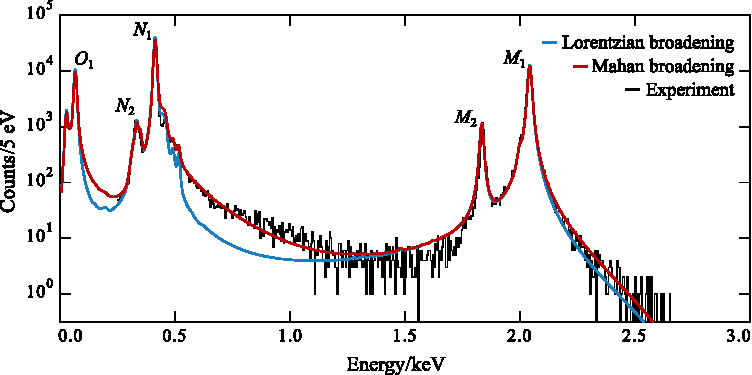
\includegraphics[width=0.75\textwidth]{figures/ch1/mahan.pdf}
  \caption{$^{163}$Ho nuclear decay spectrum measured by the Echo collaboration compared to ab initio theory broadened
  using a Lorentzian line-shape (blue) and Mahan line-shape (red). Image taken from  \cite{velte2019high}.}
  \label{fig:mahan}
\end{figure}


A more precise calculation of the spectrum requires considering second-order processes, which involve more electrons in the
decay. For example, when a second electron is promoted to another orbital, creating additional peaks, the phenomenon is
called "shake-up." If the electron escapes the atom and goes into the continuum spectrum, it is denoted as "shake-off."
The shake-off results in a broad and continuous alteration of the first-order spectrum, potentially enhancing the
statistics near the endpoint. Third and higher order processes are predicted to provide negligible
contributions \cite{thirdorder}.

More comprehensive descriptions, such as ab initio calculations, provide the best theoretical predictions available \cite{brass2018ab}. These methods reveal features beyond
the seven peaks, including shake-up and shake-off, asymmetric peak broadening, and energy shifts. The predicted
spectrum shows good but not perfect agreement with experimental data from the ECHO collaboration \cite{velte2019high}, as
shown in Figure \ref{fig:mahan}. The asymmetries appear to be mostly consistent with a Mahan broadening of the Breit-Wigner peaks, parametrized with an electron energy cutoff \(\xi\) and asymmetry \(\alpha\):

\begin{equation}
M_H(E) = \int_{0}^{\infty} L_H(E_c - E') \frac{1}{\xi \Gamma(\alpha)} \frac{e^{-E'/\xi}}{(E'/\xi)^{1-\alpha}} dE'
\end{equation}
Where \(L_H(E_c)\) denotes the Lorentzian function describing a peak in the first-order approximation. 
To allow for comparison between theoretical predictions and data, the experimental spectrum \(S(E_c)\) is obtained from
the theoretical spectrum \(S_{EC}(E_c)\) by considering pile-up events, the background, and the energy resolution of the
experiment. The pile-up spectrum is approximated as the convolution of the single spectrum with itself, multiplied by the fraction of unresolved pile-up events \(f_{pp}\). The experimental spectrum is expressed as:

\begin{equation}
S(E_c) = \left[ (1-f_{pp}-f_{bkg})S_{EC}(E_c) + f_{pp} S_{EC}(E_c) * S_{EC}(E_c) + f_{bkg}B(E_c) \right] * R_{\Delta E}(E_c)
\end{equation}

Here, \(B(E_c)\) is the background spectrum, and \(R_{\Delta E}(E_c)\) is the energy response of the detector, usually
a Gaussian, corresponding to
an energy resolution \(\Delta E\).
\section{The Holmes detector}
\subsection{Transition Edge Sensors}\label{sec:TES}

The detectors used in the Holmes experiment consist of three essential components: an absorber doped with $^{163}$Ho to convert radiation
energy into heat, a Transition Edge Sensor (TES) thermometer to translate heat into a measurable signal, and an
insulating structure to confine the energy for precise measurement before restoring the idle temperature after an event. Among Low Temperature Detectors, superconducting TESs offer high resolution and efficient multiplexing readout techniques.
A TES serves as a sensitive thermometer by operating within the narrow temperature range of the transition between the
superconductive and resistive states of a metal \cite{irwin2005TESreview}. When energy is deposited in an absorber
thermally linked
to a TES, the resulting temperature change causes a resistance variation in the
TES. If a constant voltage bias is applied, this change of resistance leads to a measurable drop in the current flowing
through the TES. Consequently, a
change in energy corresponds to an observed change in current.% The working point of a TES is usually expressed as a percentage of the normal resistivity $R_n$ of the metal, indicating at which point in the transition it has been biased.

The sensitivity of TESs arises from the sharpness of the superconductive-to-normal metal transition. However, the
complex physics of this phenomenon makes predicting the detector's behavior challenging. The resistance of a TES mainly
depends on temperature and current, denoted as $R(I, T)$, and is also weakly dependent on the local magnetic field, which can typically be neglected.
A simplified description of a voltage-biased TES can be represented by an electrothermal circuit, as shown in Figure
\ref{fig:TEScircuit}. The voltage bias is achieved by applying a constant current to a small shunt
resistance $R_{sh}$ parallel to the TES and to an inductance $L$, which corresponds to a Thevenin equivalent circuit with
constant voltage $V$ and load resistance $R_{L}=R_{sh}$. The TES, modeled as a variable resistor $R_{TES}$, is coupled to an
absorber with heat capacity $C$, exchanging heat with the thermal bath through a heat conductance $G$. The evolution of
this system is determined by two differential equations:

\begin{eqnarray}
  C \frac{dT}{dt} = -P_{\text{bath}} + P_J + P \\ \label{eq:et1}
  L \frac{dI}{dt} = V - IR_{sh} - IR_{\text{tes}} \label{eq:et2}
\end{eqnarray}

These equations couple the electrical and thermal responses through the nonlinear quantities $R_{TES} = R_{TES}(I, T)$
and $P_J = R_{TES}I^2$. Moreover, they show that operating a TES in the voltage-biased regime, where $R_{sh} \ll R_{TES}
$, offers advantages. When energy is deposited in the absorber, causing an increase in temperature and TES resistance,
the reduced current flow decreases the Joule power dissipation in the TES, restoring the initial temperature after a
short transient. This effect, known as negative electrothermal feedback (ETF), stabilizes the TES's operational state. 
\begin{figure}[t]
    \begin{subfigure}[b]{0.5\linewidth}
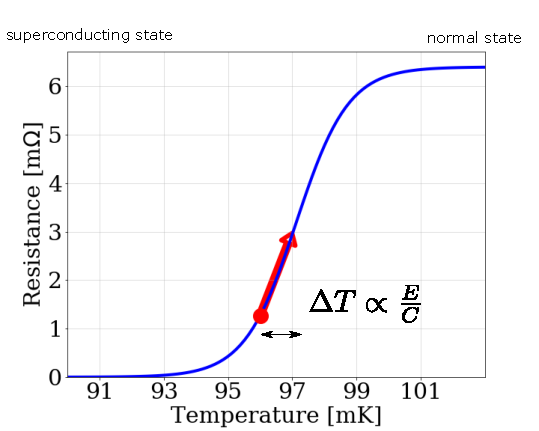
\includegraphics[width=\linewidth]{figures/ch1/TEStheory.pdf}
\caption{}
\end{subfigure}
\hspace{0.5cm}
\begin{subfigure}[b]{0.35\linewidth}
    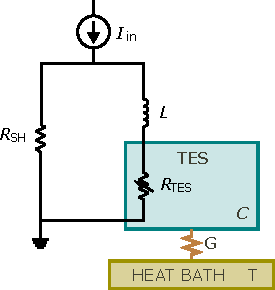
\includegraphics[width=\linewidth]{figures/ch1/TEScircuit.pdf}
\caption{}
\end{subfigure}
\caption{Operating principle of a Transition Edge Sensor (a). Electrothermal circuit diagram for a voltage
biased TES (b).} 
\label{fig:TEScircuit}
\end{figure}

The response differential equations can be solved in the small signal approximation by linearizing the resistance with a
first-order expansion, assuming that its change due to absorbed energy is small compared to
the at-rest TES state $R_0(I_0, T_0)$. Two logarithmic derivatives, denoted as $\alpha$ and $\beta$, define the sensitivity to
temperature and current changes:

\begin{equation}
\alpha = \frac{\partial \log R}{\partial \log T}\Bigg|_{I_0=T_0,R_0} \quad  \quad \beta = \frac{\partial \log R}{\partial \log I}\Bigg|_{T_0=I_0,R_0}
\end{equation}

The resistance and dissipated power can then be linearized for small deviations $\delta T = T - T_0$ and $\delta I =
I - I_0$:

\begin{eqnarray}
R(T, I) \sim R_0 + \alpha R_0 \delta T + \beta R_0 \delta I\\
P_J \equiv I^2R \sim P_{J0} + 2I_0R_0\delta I + \alpha P_{J0}\delta T + \beta P_{J0}\delta I
\end{eqnarray}

These approximations allow deriving analytical solutions for the differential equations \ref{eq:et1}. While the small signal approximation does not precisely predict the detector's response, it provides valuable information about signal parameters and noise spectrum, as well as expected energy resolution.
The noise spectrum is characterized by three main sources: the Johnson noise of the TES resistance, that of the load or
shunt resistor, and the thermal fluctuation noise. Observed additional noise has been linked to the thermal circuit
configuration, but some unexplained sources still persist.
For small signals and strong negative ETF, it can be shown that the TES energy resolution is proportional to:
\begin{equation}
  \Delta E\propto \sqrt{{4k_B T^2 C}{\sqrt{\frac{1+2\beta}{\alpha}}}}
\end{equation}
This relationship shows that optimal operation of the TES requires proper combination of temperature, current and bias
to maintain low current sensitivity $\beta$ and high temperature sensitivity $\alpha$ \cite{zhou2020towards}. 

A more comprehensive treatment of the TES response in the large signal regime requires an understanding of the mechanisms
underlying the superconducting transition. For larger TES devices, such as those used in the Holmes detector,
experimental observations are consistent with a two-fluid model featuring Phase Slip Lines (PSLs) \cite{PSLcenters}. In the context of
superconductivity, the macroscopic wave function of the Cooper pairs $\psi(r) = |\psi(r)|e^{i\phi(r)}$ serves as the
order parameter. This order parameter exhibits amplitude and phase coherence, which disappear at the critical
temperature or current, marking the transition to the normal phase.
\begin{figure}[t]
\begin{subfigure}[b]{0.4\linewidth}
    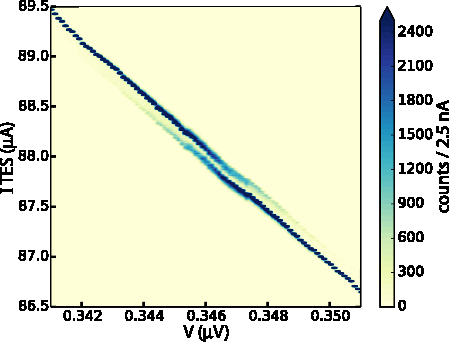
\includegraphics[width=\linewidth]{figures/ch1/PSL1.pdf}
    \caption{}
  \end{subfigure}
\hfill
\begin{subfigure}[b]{0.5\linewidth}
    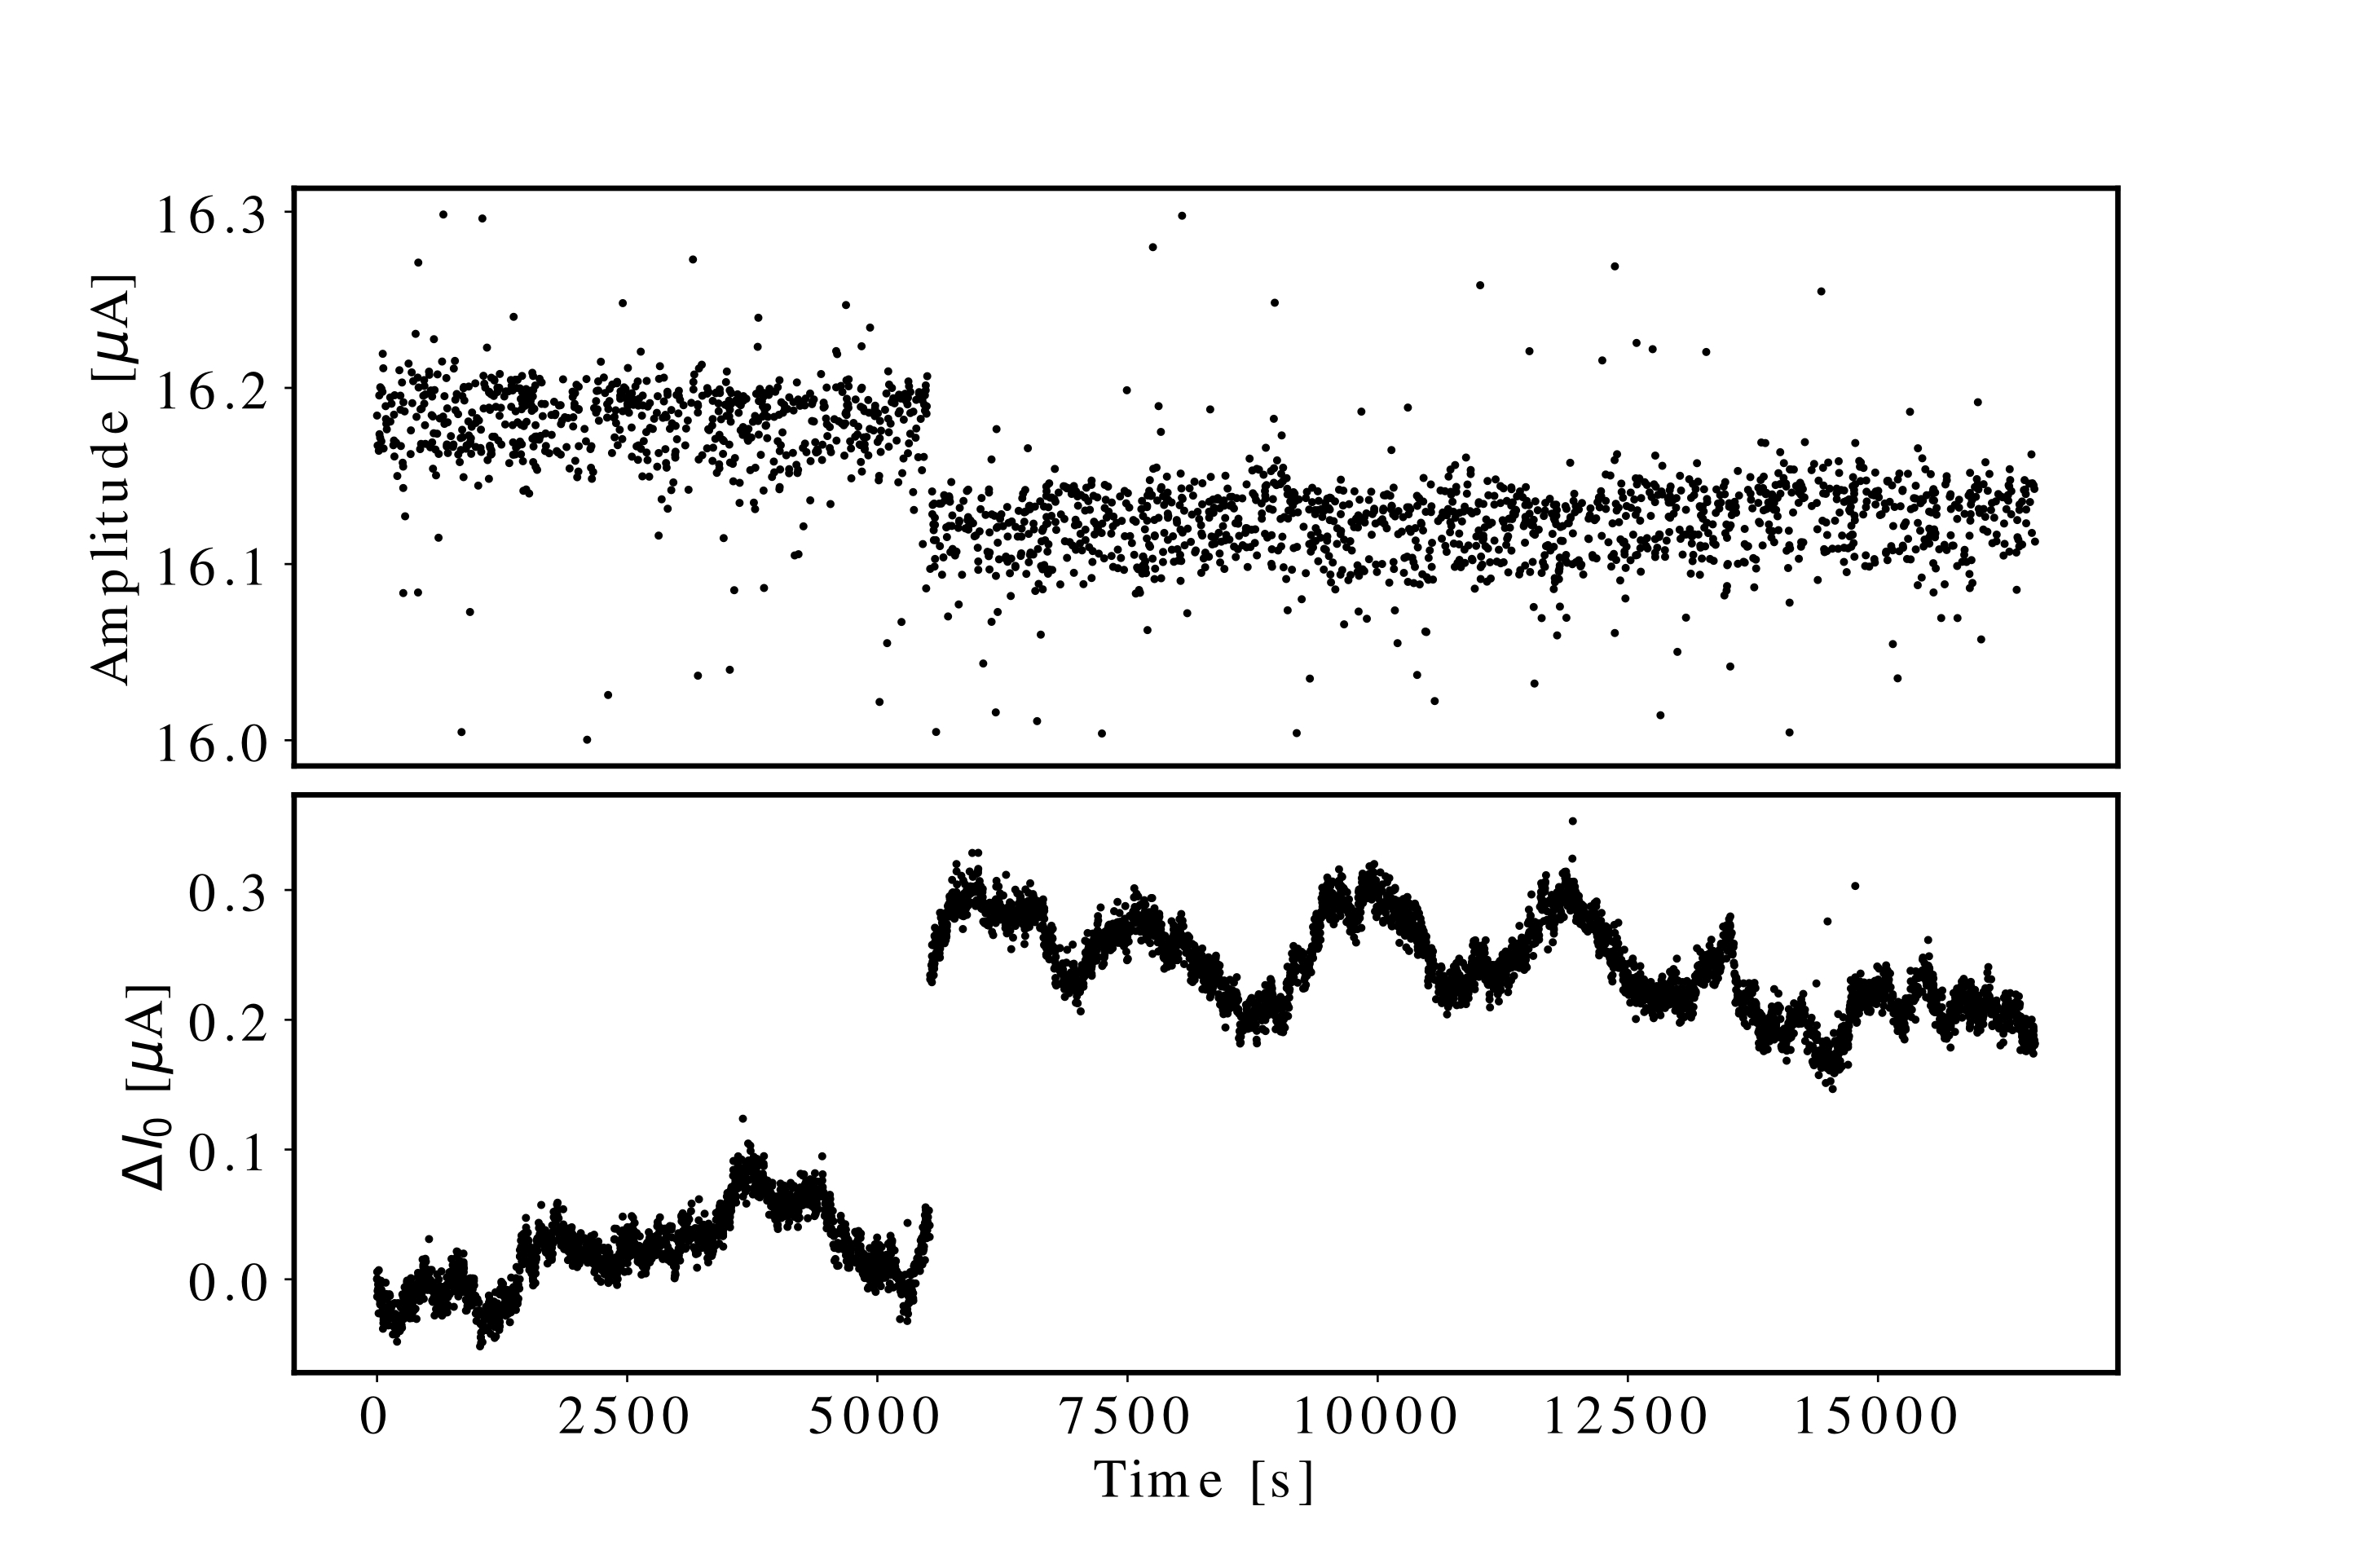
\includegraphics[width=\linewidth]{figures/ch1/PLS2.jpg}
    \caption{}
  \end{subfigure}
  \caption{Measured IV characteristic of a TES. For each bias voltage, 130000
    measurements of the current are histogrammed (a). Image taken from  \cite{PSL}. Sudden variation in the idle current of the TES
used by the Holmes experiment, resulting in different signal amplitude for events originating from an approximally
monochromatic X-ray source (b). Image taken from  \cite{borghesi2022toward}}
\label{fig:PSL}
\end{figure}
This transition does not occur uniformly across the entirety of the superconducting material. Instead, phase slips
manifest as localized regions within the superconductor where the current surpasses its critical value and becomes
partially carried by quasi-particles, thereby generating a potential difference. Along the boundaries of these phase
slips, two supercurrents with distinct order parameters emerge. In filamentary superconductors, phase slips correspond
to nucleation centers, whereas in two-dimensional films, they appear as lines perpendicular to the direction of current
flow. For a given voltage drop across the TES, different numbers of phase slip lines $n_{PSL}$ can be present, resulting
in multiple potential values of observed current. This phenomenon leads to bimodal structures in the current-voltage (IV) curve.
These predictions can be experimentally verified  \cite{PSL}, as illustrated in Figure \ref{fig:PSL}.
Furthermore, the model provides insight into another phenomenon observed in the Holmes detectors, where the signal
amplitude of the TES for events with approximately the same energy abruptly changes and remains in this altered state
for several minutes. This behavior may be attributed to the fact that, on occasion, the detector settles into a stable
state characterized by a different number of PSLs compared to the initial state before the event \cite{borghesi2022toward}.



\subsection{Microwave Multiplexing readout}\label{sec:muMUX}
Since a substantial
number of microcalorimeters is needed for a meaningful measurement of $m_{\nu_{e}}$, the readout system must provide a
high multiplexing factor while maintaining a fast signal response to limit pile-up events. Multiplexing refers to the ability to read
multiple detectors with a single electrical connection within the cryostat.
Its primary objective is to shift the complexity of the experimental setup outside the cryostat to the warm stage. 
Without multiplexing, the number of wire
pairs required to operate all the TESs employed by Holmes would be unmanageably high, leading to excessive heat generation at the cryogenic stage.

In recent years, Microwave SQUID Multiplexing ($\mu$MUX) has emerged as a practical and consistent method for reading arrays
of microcalorimeters, satisfying the necessary requirements and outperforming other multiplexing techniques such as time
or frequency division multiplexing \cite{muMUX}.
The $\mu$MUX readout chip comprises a series of quarter-wave resonators, each coupled to an rf-SQUID (radio-frequency
Superconducting Quantum Interference Device), which is used to adjust their resonant frequencies. An rf-SQUID consists
of a superconducting loop interrupted by a single Josephson junction, a circuit element with no classical
equivalent consisting of two overlayed superconducting terminals separated by a thin insulator. The
response of a Josephson junction is determined by the tunneling of Cooper pairs through the barrier and can be described
as a nonlinear inductance dependent on the phase difference $\phi$ between the wavefunctions at the junction's sides:

\begin{equation}
L(\phi) = \frac{L_J}{\sin\phi}, \quad L_J= \frac{\hbar}{2eI_c}= \frac{\Phi_0}{2\pi I_c}
\end{equation}
Here, \(I_c\) represents the critical current of the superconductor and \(\Phi_0\) denotes the magnetic flux quantum.
When the self-inductance of an rf-SQUID \(L_S\) is less than that of the Josephson junction \(L_J\), the loop functions as an extremely sensitive magnetometer. The phase difference becomes proportional to the magnetic flux through the loop:

\begin{equation}
  \phi=\frac{2e}{\hbar}\int\left(\frac{d\Phi}{dt}\right)dt =2\pi\frac{\Phi}{\Phi_{0}}
\end{equation}
A variation in flux leads to a change in current and voltage drop across the junction, which depend on the phase and
its time derivative:
\begin{equation}
  \frac{2e V}{\hbar} = \frac{d\phi}{dt}, \quad I = I_c \sin\phi
  \label{eq:JJ}
\end{equation}
The rf-SQUID can be read by inductively coupling it to another circuit, the impedance of which is then dependent on variations
of the observed flux. In the case of the $\mu$MUX chip, each rf-SQUID is coupled to a resonator designed to
ring at a unique frequency. Many resonators are coupled to a common feedline, allowing for their
simultaneous readout by sending through
the feedline a combination of fixed gigahertz signals at the resonating frequencies. Changes in the flux applied to a SQUID result in changes of the corresponding resonator's impedance and resonant
frequency, which manifest as shifts in the phase and amplitude of the probe signal at the specific frequency.
The phase signals are larger than those in amplitude, and the latter are usually discarded.
In this way, rf-SQUIDs amplify the weak signal currents generated in a TES, while the resonators enable to differentiate each microcalorimeter using a distinct frequency.

In summary, an energy deposition in a voltage-biased TES results in a change in its resistance and current flow,
typically in the order of tens of microamperes. Through the TES circuit's
inductance, this current generates a magnetic flux that is read and amplified by an rf-SQUID, altering the resonant frequency of the corresponding resonator.
When the resonator is probed at a fixed frequency, this results in an observable signal, which is read as a phase difference in the circuit's response.

This setup is further complicated by the fact that the SQUID's response to changes in magnetic flux is periodic rather
than linear, as can be seen from Eq \ref{eq:JJ}. Therefore, a method called flux ramp
modulation is employed to linearize the SQUID's response \cite{mates2012flux}. Figure \ref{fig:multireadout} depicts the complete multiplexing and readout circuit for Holmes,
including voltage bias and flux modulation.
\begin{figure}[t]
  \centering
  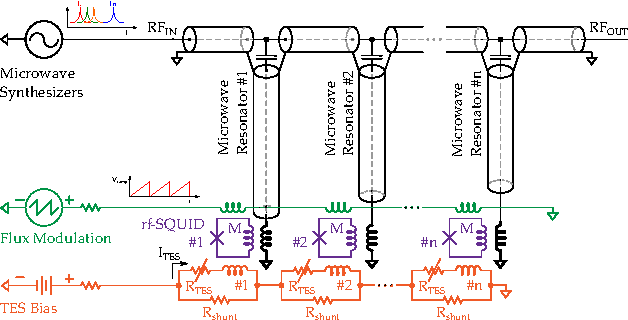
\includegraphics[width=0.8\textwidth]{figures/ch1/HOLMEScircuit.pdf}
  \caption{Circuit diagram of the multiplexing and readout scheme used by Holmes.}
  \label{fig:multireadout}
\end{figure}
In this modulation scheme, a common flux ramp signal is applied to all SQUIDs. The flux ramp is a sawtooth signal that resets at a frequency of \(f_{\text{ramp}}\) and has an amplitude set to induce integer multiples of flux quanta (\(n\Phi_0\)) in the SQUIDs, causing them to perform identical and periodic oscillations during each ramp cycle.
If the frequency of the applied ramp exceeds the maximum frequency content of any input signal, a change in the TES
current ad thus a variation of the SQUID input corresponds to a phase offset in the SQUID's ramp-induced oscillation.
This phase shift is directly proportional to the magnetic flux through the loop and can be measured using a Fourier
transform of the observed SQUID oscillation.
At each ramp cycle, the SQUID response $S(t)$ is sampled a certain number of times. Then, the phase offset is obtained
by performing a Fourier measurement between the samples:
\begin{equation}
I \propto \phi = \arctan\left(- \frac{\sum S(t) \sin(2\pi n\Phi_0 f_{\text{ramp}} t)}{\sum S(t) \cos(2\pi n\Phi_0 f_{\text{ramp}} t)}\right)  
\end{equation}
In this way, the TES signal is sampled with frequency $f_{ramp}$, once every ramp cycle.
This parameter must be chosen carefully to obtain an adequate number of samples during the rise time of the TES pulse,
typically around 10, while avoiding degradation of the detector's intrinsic energy resolution. The maximum sampling
frequency thus sets a limit on the speed of the detector response. 

The number of detectors that can be read simultaneously using this readout system, known as the multiplexing factor
\(N_{\text{det}}\), is limited by the total frequency range available, denoted as the bandwidth \(BW\):

\begin{equation}
N_{\text{det}} = \frac{BW}{f_{\text{ramp}} \cdot n\Phi_0 \cdot K \cdot 2} 
\end{equation}
Here, \(K\) is a "guard factor" proportional to the resonance spacing, designed to prevent crosstalk between adjacent
resonances characterized by width $BW_{\text{res}}$:

\begin{equation}
K = \frac{f_{\text{res}, n+1} - f_{\text{res}, n}}{BW_{\text{res}}}   
\end{equation}
Holmes employs the $\mu$mux17a, a 33-channel multiplexing chip developed and fabricated at the National Institute for
Standards and Technology (NIST, Boulder, CO, USA). It features a total bandwidth of \(BW = 550\) MHz, a resonance
bandwidth of approximately \(BW_{\text{res}} \approx 2\) MHz and resonance spacing of 14 MHz, corresponding to $K=7$.
With a ramp frequency of 500 kHz and two SQUID oscillations per cycle, this results in a multiplexing factor of approximately \(N_{\text{det}} \approx 39\).

\subsection{Detectors design and fabrication}\label{sec:fabrication}
Each TES in the Holmes detectors consists of a $125\times125\mu \text{m}^2$ metal bilayer composed of molybdenum
and copper, which suppresses the critical temperature of Mo from 920mK to 100mK. The bilayer features copper bars
oriented orthogonally to the current flow which have been shown to reduce excess electrical noise and allow to tune the
normal resistance $R_n$.
A gold absorber measuring 180 × 180 × 2 $\mu m^3$ is chosen to provide high stopping power, low heat capacity, and efficient
thermalization properties. The de-excitation products of Ho decay, such as Auger electrons and X-rays, undergo
relaxation through electron-electron and electron-phonon scattering interactions within a fraction of a nanosecond. It is
predicted that the chosen absorber thickness allows for a 99.99\% probability of stopping electrons and a 96.73\%
probability of stopping photons from the decay.
As the Au absorber is deposited atop a copper structure with a connecting bar to the TES, their temperature become closely coupled, ensuring thermal equilibrium between the two components.
The current design of the Holmes detector, shown in Fig \ref{fig:TES}, employs a sidecar geometry to mitigate the proximity effect between the
thermal sensors and the absorber, which could otherwise alter the resistance profile in the transition.


\begin{figure}[!b]
    \begin{subfigure}[b]{0.3\linewidth}
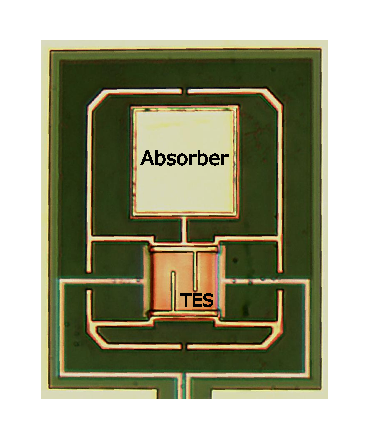
\includegraphics[width=\linewidth]{figures/ch1/TES.pdf}
\caption{}
\end{subfigure}
\hspace{1.5cm}
\begin{subfigure}[b]{0.55\linewidth}
    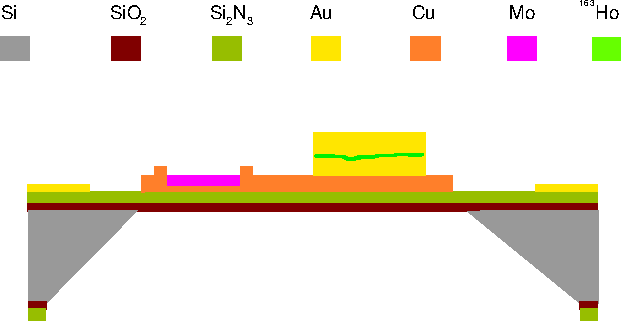
\includegraphics[width=\linewidth]{figures/ch1/TESdesign.pdf}
\caption{}
\end{subfigure}
\caption{Top view of a microcalorimeter used by the Holmes experiment, showing an absorber and TES suspended over a
thin Si$_2$N$_3$ membrane, which appears dark in the photo (a). Side view of the detector, illustrating the different
materials used in the current design (b). The figure is not to scale.} 
\label{fig:TES}
\end{figure}
Achieving thermal isolation of the detector is crucial for measuring all the energy released in an event and tailoring the signal time profile to match the readout
system's bandwidth and sampling frequency. The detectors used by Holmes are positioned on a suspended silicon nitride Si$_2$N$_3$
membrane, preventing the escape of hot phonons during the thermalization process. The
membrane's thickness is approximately 500 nm. 

Moreover, to minimize experimental dead-time, the heat dissipation from the perimeter of the detector to the thermal bath is enhanced with a thin copper trace around the detector. This has been demonstrated to
increase the thermal conductance while minimally affecting heat capacity, thus preserving energy resolution.
The detectors fabrication undergoes three phases: 
\begin{description}
  \item[Array fabrication at NIST:] After having produced the bare circuit for a 64 detectors array with standard techniques, a photoresist
    mask exposing only the absorbers is applied and the first $1\mu$m of gold is deposited over the photoresist.
  \item[Ho production and implantation:]
The necessary $^{163}$Ho must be synthesized through thermal neutron irradiation. Enriched $^{162}$Er$_2$O$_3$ powder
was irradiated at the ILL nuclear reactor in Grenoble, France, with the resulting $^{163}$Er decaying to $^{163}$Ho via electron capture. 
\begin{equation}
^{162}\text{Er}(n, \gamma)^{163}\text{Er} \rightarrow ^{163}\text{Ho} + \nu_e
\end{equation}
To ensure the purity of the obtained holmium, chemical purification processes were conducted at the Paul Scherrer
Institute, yielding approximately a total of 200 MBq of $^{163}$Ho.
A custom ion implanter housed in Genoa, which will be discussed in more detail in the next section, is used to
incorporate the $^{163}$Ho nuclei into the TES absorbers. The core component
of the implanter is a sputter ion source that generates argon plasma from thermoionic electrons. The plasma exctracts Ho ions from a
target, and the obtained ions are accelerated and collimated in a beam. Subsequently, a magnetic selector,
consisting of a dipole magnet, separates the $^{163}$Ho ions from other contaminants before projecting the beam onto the TES
array.  

\item[Array finalization in Milan:] The final $1\mu$m of gold is deposited over the implanted detectors with a system
    consisting of four Compact Microwave and Coaxial (COMIC) ion sources placed in a high
vacuum environment, denoted as the target chamber. Each COMIC source uses an electric field generated by antennas within a magnetic cylinder to ignite
an argon plasma, which is used to create four focused argon ion beams directed at ultra-pure gold targets, depositing
part of the sputtered gold on the detectors array. The excess gold is then removed with the lift-off of the
photoresist mask by dipping the array in acetone. 
Finally, the thin Si$_2$N$_3$ membranes over which the TES are suspended to achieve thermal isolation are exposed with a KOH
etching process. A potassium hydroxide solution is used to etch silicon, producing almost vertical
walls. The technique provides consistent results, and the etched areas exhibit good uniformity and quality.
\end{description}





\section{Experimental setup}\label{sec:setup}
\subsection{Detector holder and calibration sources}\label{sec:holder}

\begin{figure}[t]
    \begin{subfigure}[b]{0.68\linewidth}
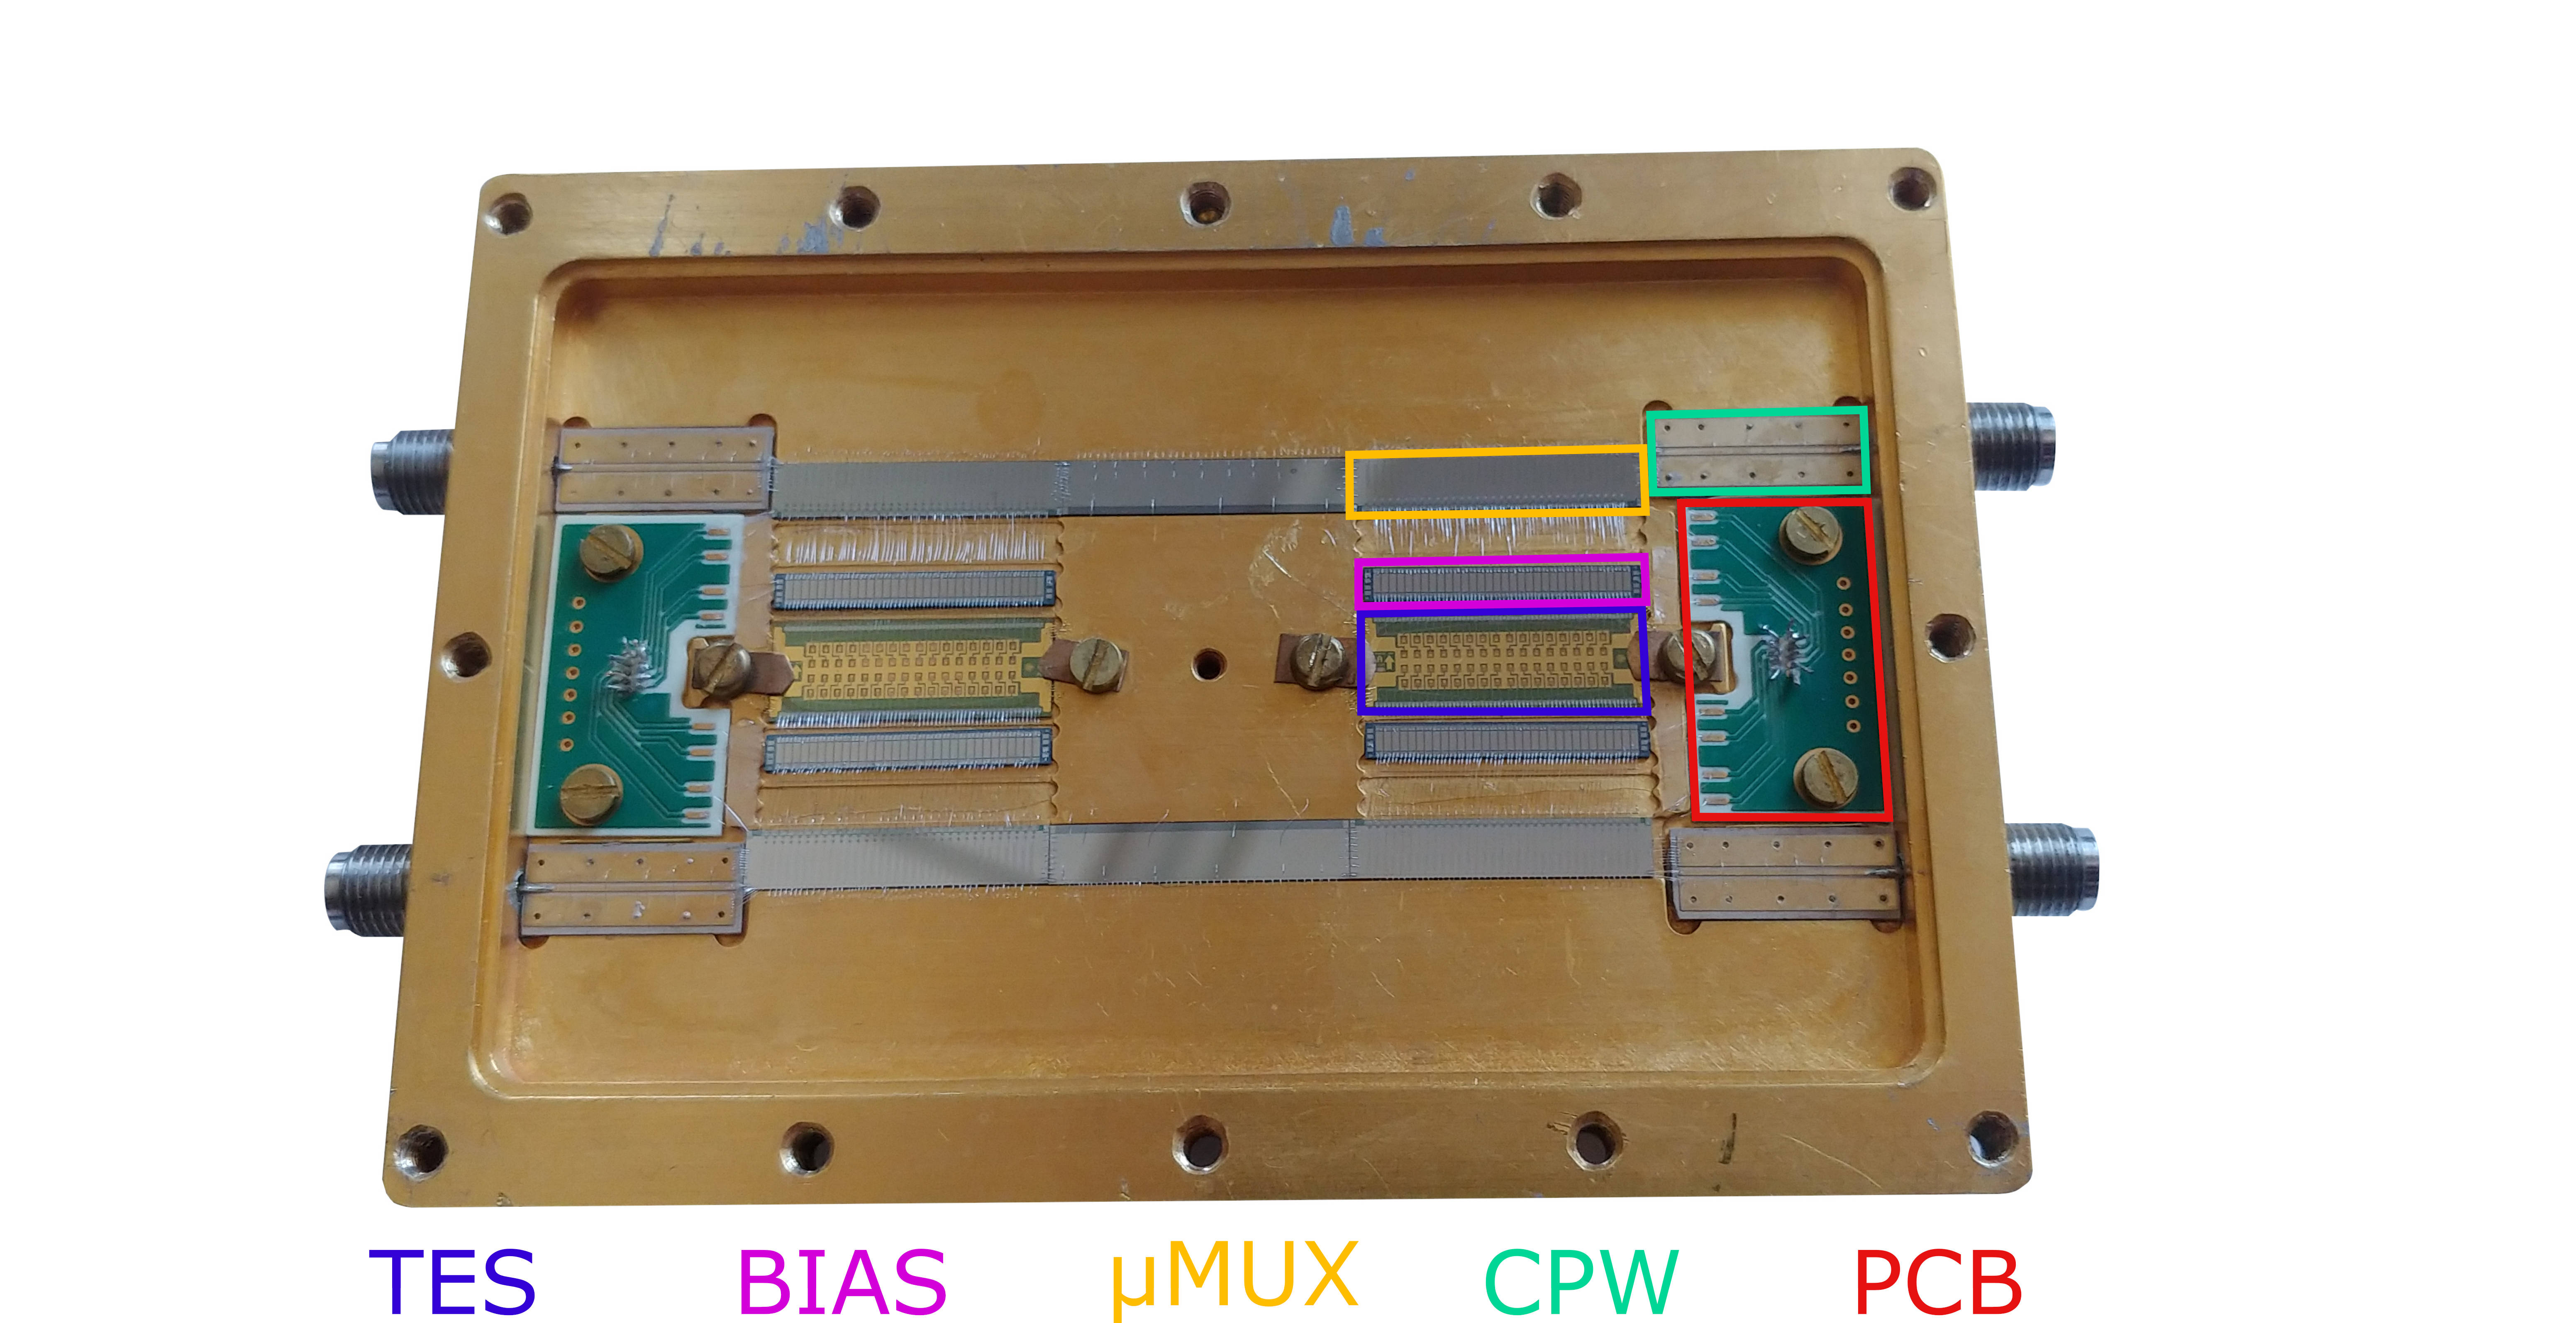
\includegraphics[width=\linewidth]{figures/ch1/holderfi.jpg}
\caption{}
\end{subfigure}
\begin{subfigure}[b]{0.3\linewidth}
    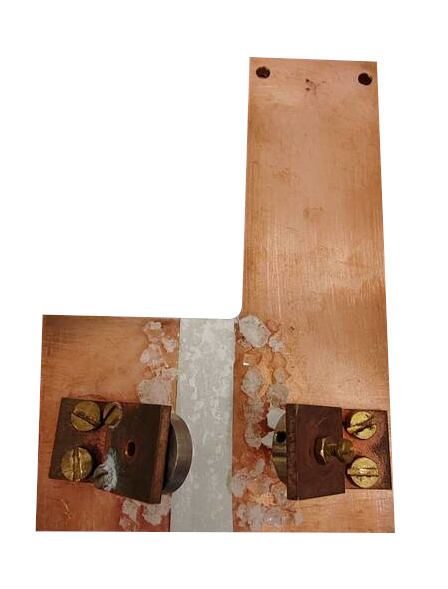
\includegraphics[width=0.9\linewidth]{figures/ch1/calcrop.jpg}
\caption{}
\end{subfigure}
\caption{Detector holder housing the TES arrays and microwave multiplexing system (a). Example of X-ray calibration
source. Two $^{55}$Fe samples are directed at NaCl crystals and CaCO$_3$ powder glued to a copper plate (b).} 
\label{fig:holder}
\end{figure}
The TES arrays and multiplexing chips are accomodated in a holder measuring 10.5 × 7.5 × 0.85 cm$^3$, constructed from
gold-plated copper to prevent oxidation and maintain high thermal conductivity. The holder allows containing up to two
TES arrays, totaling 128 detectors with their respective readout and bias chips, which are connected through aluminum wire bondings.
The setup used in the first measurement campaign with $^{163}$Ho, shown in Fig \ref{fig:holder}, contains the following components:
\begin{description}

\item[TES array]: Each TES chip comprises 2 modules of 32 detectors,
  with bonding pads for bias on both sides. Various Au bonds (25 or 50 $\mu$m diameter) thermalize the gold plates around the detectors to the holder.
  
\item[Bias chip:] Each TES is connected in parallel with a small resistance ($R_{sh}$) of 0.3 m$\Omega$. The long bonding
  wires connecting this chip to the detectors introduce stray inductance that slows the TES signals, allowing them to
  be measured with the multiplexing configuration.


\item[Multiplexing chip:] The readout chip is a $\mu$mux17a multiplexer chip optimized for Holmes, featuring 33
  quarter-wave resonators coupled to rf-SQUIDs made from 200 nm thick Nb film on high-resistivity silicon. 

\item[Printed Circuit Board:] The PCB has 8 available pins, allowing to connect the ramp and TES bias to the chips at either sides of the array.

 \item[Coplanar Waveguides:] The CPWs are used to bring RF signals to the $\mu$MUX chip.
\end{description}
Due to the multiplexing factor, each array of 64 TESs requires two $\mu$MUX chips, resistance chips and coplanar waveguides. 

The holder cover features two holes above the detector arrays, covered with 6 $\mu$m thin aluminum foil to block external
thermal radiation while allowing X-rays to reach the detectors. This setup enables the use of an X-ray source in close
proximity to the holder for energy calibration. A source consisting of \(^{55}\)Fe pointing at a mixture of NaCl and
CaCO\(_3\) is employed. The \(^{55}\)Fe undergoes electronic capture, and the resulting X-rays can be measured by the
detectors or generate other X-rays through the fluorescence of calcium, chlorine, and aluminum from the impacted
materials. After calibrating the detectors with a dedicated run, the source must be removed to observe only the Holmium. The development of a switchable calibration source is currently in progress.


\subsection{Cryogenics setup}

A $^3$He/$^4$He dilution Triton refirgerator by Oxford Instruments, shown in Fig \ref{fig:cryo},  is used to operate the
TESs at temperatures of
60-80mK. \begin{figure}[!b]
    \begin{subfigure}[b]{0.45\linewidth}
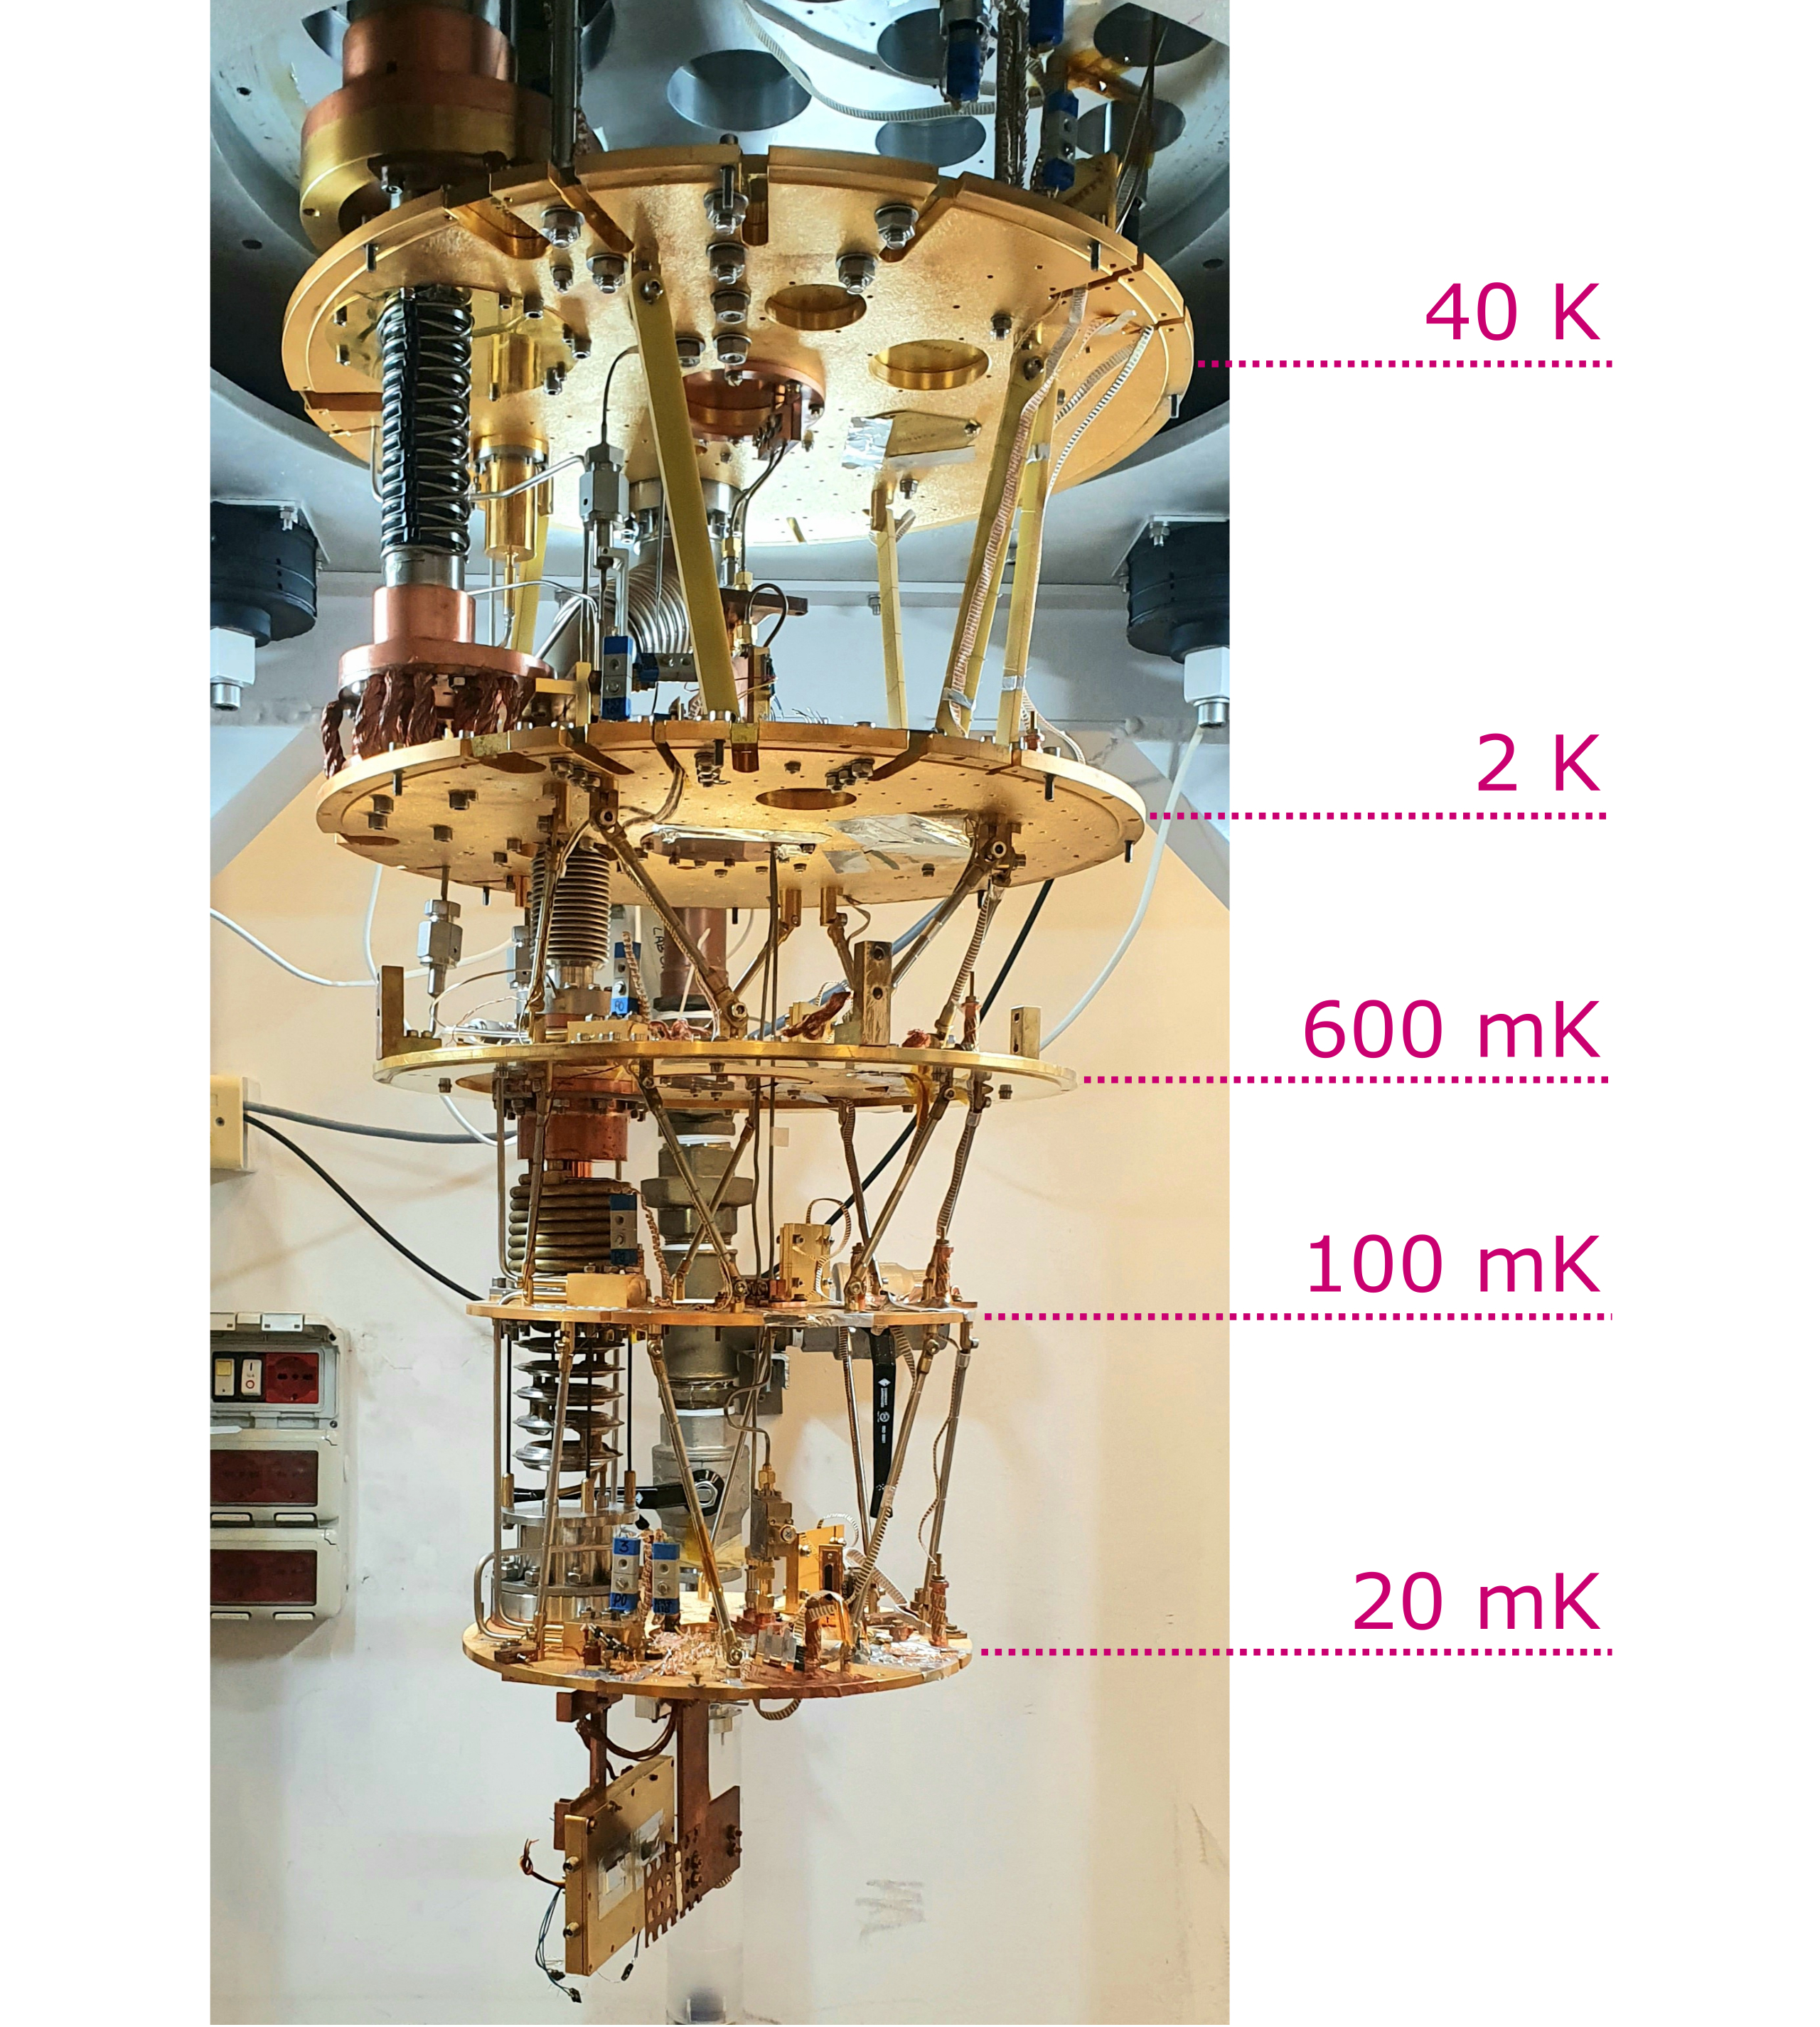
\includegraphics[width=\linewidth]{figures/ch1/cryo.jpg}
\caption{}
\end{subfigure}
\hfill
\begin{subfigure}[b]{0.45\linewidth}
    \includegraphics[width=\linewidth]{figures/ch1/holder.jpg}
\caption{}
\end{subfigure}
\caption{The dilution refrigerator used by Holmes (a). Close-up of the detectors holder mounted to the mixing
chamber's plate (b).} 
\label{fig:cryo}
\end{figure}
To achieve the required vacuum level of around $10^{-6}$ mbar, a diaphragm pump and a turbomolecular pump are employed. A series of thermal shields made of aluminum and copper are securely fastened to different plates to prevent thermal radiation from transferring between the various temperature stages.
Since the rf-SQUIDs are highly sensitive magnetometers, a substantial magnetic shield is mounted and connected to the
second-stage 2K plate. The detectors holder is attached to a copper plate under the coldest
refrigeration stage, the mixing chamber plate, and further thermalized with copper braids. 


The microwave probe tones used for the multiplexed readout must travel from the warm 300K electronics to the 60mK cold
stage where the $\mu$MUX chip is located. Copper-nickel coaxial cables are used for this purpose between 300K and 4K.
After a 20 dB attenuation at 2K to match thermal noise levels, the signal is transmitted
through stainless steel cables and undergoes another 20 dB attenuation before entering the detetors holder. Upon exiting
the box, it passes through a circulator that shields the detectors from the noise generated by the following amplification stage, which uses a low-noise High Electron Mobility
Transistor amplifier (HEMT) placed on the 2K plate. In this stage,
connection is established using superconducting Nb coaxial cables to avoid signal dissipation and ensure minimal thermal
conductance, while the amplifier models (LNF - LNC48A) offers optimal noise performance in the working frequency range
of 4-8 GHz. 
The voltage ramp signal required for $\mu$MUX multiplexing demodulation and the voltage bias for the detectors are transmitted using Nb-Ti twisted pairs, which are themselves thermally linked to each temperature stage through contact, forming a ribbon on a small copper rod fastened to each plate.
Various heaters and thermometers are distributed across the different plates, allowing for comprehensive monitoring and control of the cryostat's behavior during measurements.



\subsection{Warm electronics setup}
The system for the multiplexed readout of the detectors is built upon electronics initially developed for the readout of
Microwave Kinetic Inductance Detectors (MKIDs). The probe tones are generated in the Mhz range, then up-converted to Ghz with an IQ mixer and read using an heterodyne readout scheme. The main components of
this setup are:
\begin{description}
\item[ROACH2:] Denotes the 2nd-generation Reconfigurable Open Architecture Computing Hardware (ROACH2) platform.
This system consists of a digital board housing a Xilinx Virtex 5.1 FPGA for signal processing and a PowerPC
440EPx for slow control, which are paired with a peripheral DAC/ADC board hosting two DACs (1000 MS/s, 16 bit, 75 dBc of NSD) and two ADCs (550 MS/s, 12 bits, 64 dB of SNR) for generating and acquiring in-phase and quadrature signals.
Sinusoidal probe tones, one for each microresonator to be readout, are generated by the DACs using a Direct Digital
Synthesizer (DDS) and an external clock source, which is provided by a Valon synthesizer, resulting in I and Q
components with a baseband frequency range of 10-512 MHz.
Moreover, the FPGA firmware implements some fundamental processing algorithms such as the channelization of
different frequencies of the signal and the sampling of the flux ramp modulation through Fourier measurements.
The acquired data are transmitted from the ROACH2 board to a workstation computer via a 10 Gb/s Ethernet connection.

\item[IQ mixer] 
An IQ mixer is a fundamental device used in radio frequency and microwave
systems. It combines two input signals, typically a local oscillator (LO) signal and a radio frequency (RF) signal, to
generate two output signals: the in-phase (I) and quadrature (Q) components. These components represent the real
and imaginary parts of a complex signal oscillating with a frequency given by the difference bewteen that of the RF and
the LO. Alternatively, a low frequency signal with given I and Q can be modulated to the RF band by mixing it with
the LO. The heterodyne readout scheme employs both of these techniques. Up-conversion to the RF frequency range (4-8 GHz)
suitable for the multiplexer chip is achieved by mixing the I and Q generated by the ROACH2 with the LO. The IQ mixer
used by Holmes is a PXIe Hybrid with a design customized for the 4-8 GHz frequency range, matching the HEMT
bandwidth for reduced signal loss.
The modulated output tones are amplified with a gain of 26 dB and then down-converted from RF to baseband using the same
board and LO signal. The output signals I and Q are then amplified again to fully utilize the dynamic range of the two ADCs.

\item[Bias and flux ramp:]
These components play critical roles in signal reconstruction and detector stability.
The voltage bias employs a very stable power supply constructed from two large batteries, providing
stability up to ppm/$^\circ$C for the operating voltage of $\sim 500mV$.
The ramp is created by a standard signal generator. To minimize disturbances, such as ground loops and electromagnetic
interference, a custom coupling transformer is used between the signal generator and the input of the cryostat.

\end{description}
The electronics configuration is shown in Fig \ref{fig:warmelrctronics}. To synchronize all the components (ADCs, DACs,
FPGAs, and LOs), a common external clock is provided by a 10 MHz rubidium frequency standard. In the current
configuration, the ROACH2, IQ mixers, HEMT and external amplifiers are doubled to allow for the simultaneous readout of up to 64
detetctors.

\begin{figure}[t]
  \centering
  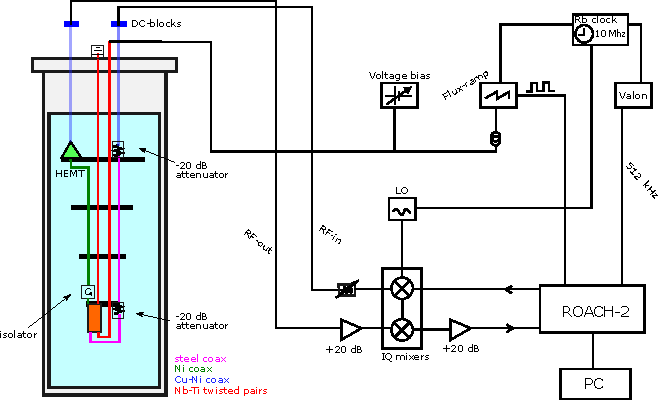
\includegraphics[width=0.74\textwidth]{figures/ch1/warmcircuit.pdf}
  \caption{Electronics circuit for the Holmes experiment. The current setup empoys two ROACH2 and four IQ mixers to read
  up to 64 detetctors at the same time.}
  \label{fig:warmelrctronics}
\end{figure}

\subsection{First $^{163}$ Ho implantation}
In its current configuration, shown in Fig \ref{fig:implanter}, the implanter consists of a Danfysik Model 921 A sputter ion
source, a 1 T magnetic dipole mass analyzer, a slit for geometrical selection, a Faraday cup for beam diagnostics and a target holder. 

In the ion source, four hot tantalum wires emit electrons through thermionic emission. These electrons are then
accelerated by a discharge potential and traverse an argon gas, creating a plasma. This plasma is then accelerated by a sputtering potential towards an electrode disk where a suitable Holmium target is situated.
The sputter target consists of a Zr/Bi (98\%/2\%) sintered matrix on which a 
$^{163}$Ho(NO$_3$)$_3$ solution is dripped to obtain an uniform distribution.
The argon ions sputter off Holmium and the other materials comprising the target. Once the Holmium atoms are
ionized by interaction with the plasma, they are accelerated by an extraction voltage ranging from 30 to 50 kV and exit the source in an ion beam, alongside the argon ions and other contaminants present on the target and in the chamber.
Subsequently, the ions pass through a small magnet capable of bending the beam along the z-axis for alignment before
entering the magnetic selector, which separates and isolates $^{163}$Ho from
other contaminants. The primary contaminant is $^{166m}$Ho, a byproduct of the $^{163}$Ho production process that decays with a
low-energy beta spectrum.
The purified Ho beam is then directed through a slit, trimming the beam tails and further reducing the likelihood of
other contaminants reaching the detectors, and Faraday cup, which measures the beam's current. Finally, the beam
reaches the TES arrays, which are mounted onto a target holder that can be moved vertically.

\begin{figure}[t]
    \begin{subfigure}[b]{0.44\linewidth}
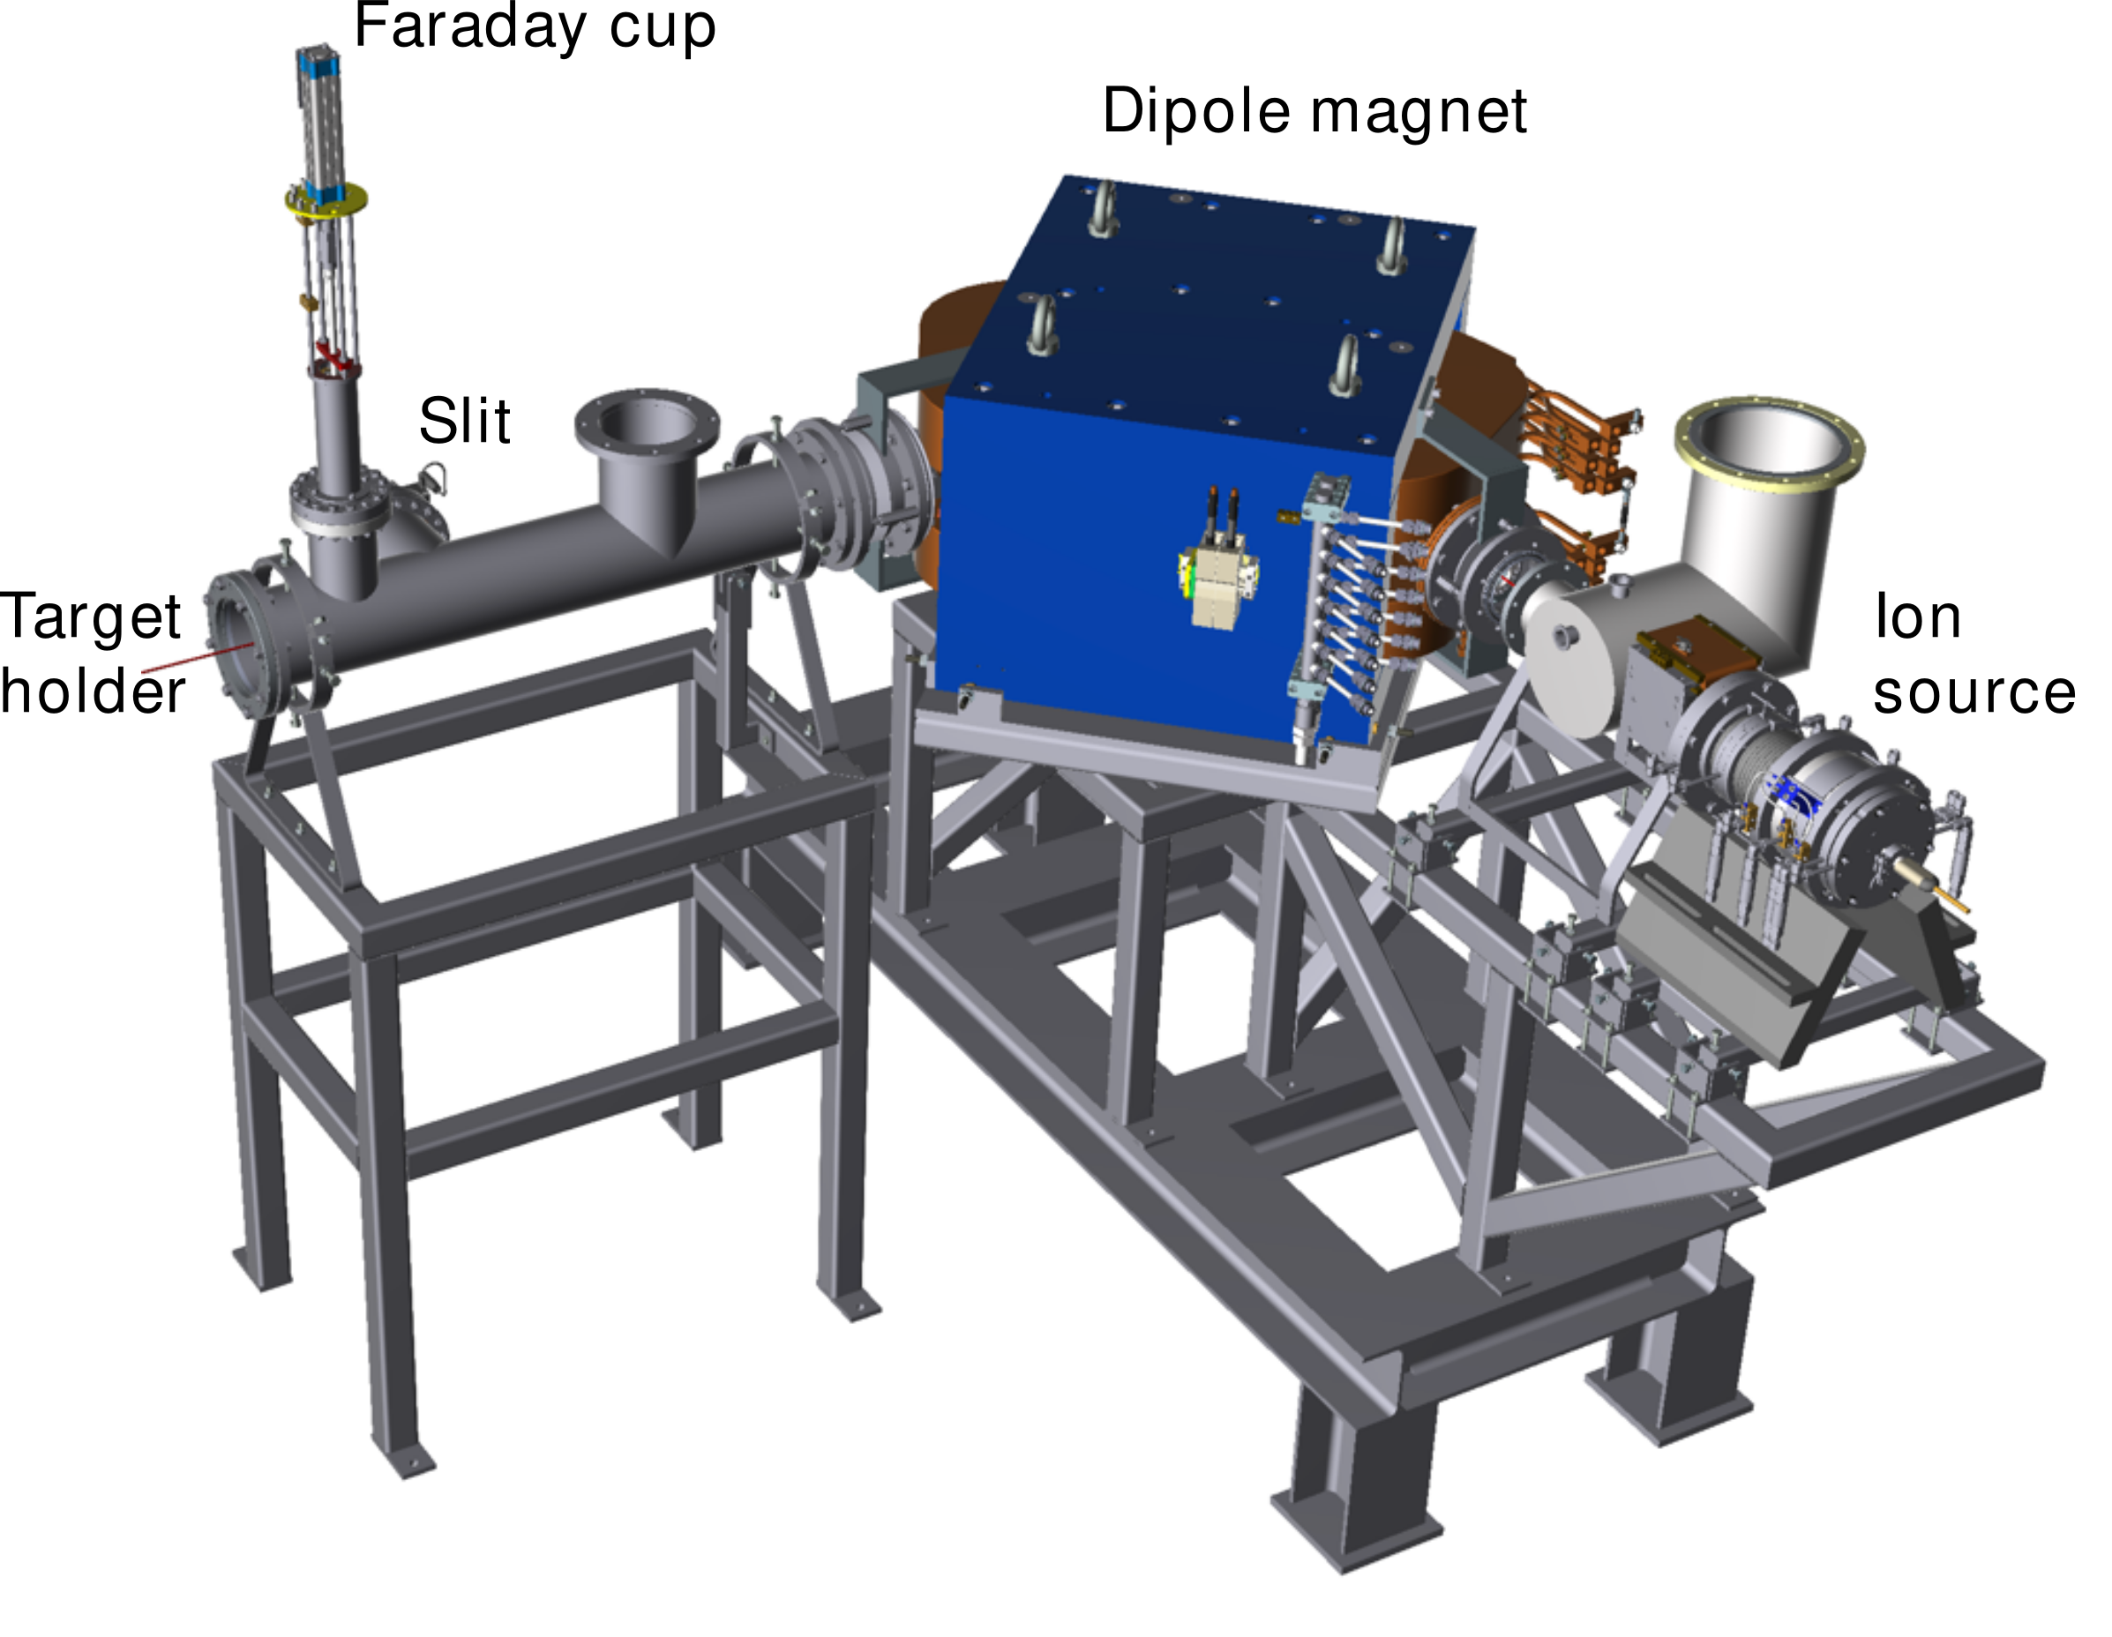
\includegraphics[width=\linewidth]{figures/ch1/implanter.pdf}
\caption{}
\end{subfigure}
\hfill
\begin{subfigure}[b]{0.4\linewidth}
    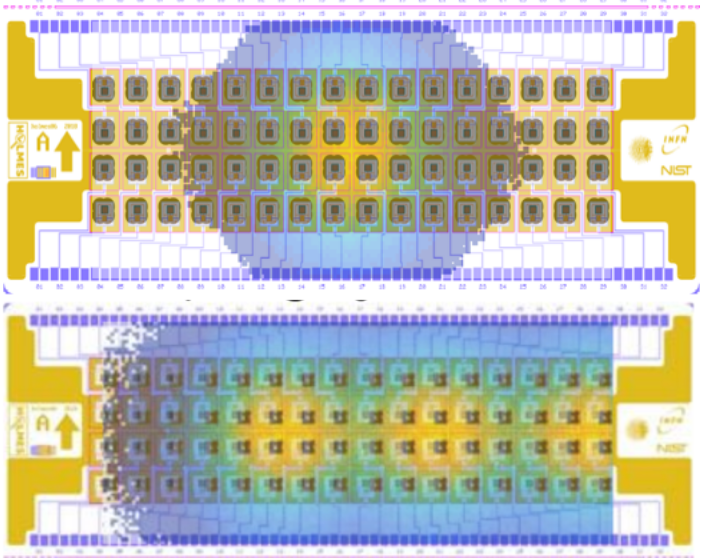
\includegraphics[width=\linewidth]{figures/ch1/implantationMC.png}
\caption{}
\end{subfigure}
\caption{Custom ion implanter used to embed $^{163}$Ho in the gold absorbers of the detector arrays (a). Monte Carlo
simulations of the expected implanted Ho distributions over the detectors for the first measurement campaing of Holmes
(b).}  
\label{fig:implanter}
\end{figure}
Looking ahead, there are plans to enhance the capabilities of the implanter. This includes the incorporation of an
electrostatic triplet and magnetic XY scanning to provide greater beam focus and control over its direction.
Simultaneously, the target chamber described in Sec \ref{sec:fabrication} will be added to the end of the apparatus, enabling Holmium implantation while
depositing gold on the absorbers. This dual function aims to achieve higher activity levels and embed the radioactive source in the full volume of the absorber rather than in a single layer.

After a series of calibration and characterization runs with $^{165}$Ho \cite{Hoimplant}, the custom ion implanter has
been utilized with $^{163}$Ho for the first time. The current implantation efficiency is anticipated to be approximately
0.2\%. Despite this small value, it remains suitable for a low-dose implantation.
Two sets of 64-TES arrays were implanted, each following a distinct pattern as shown in the simulations of Fig
\ref{fig:implanter}. The first array was targeted at a single
central spot to evaluate the beam profile and assess the impact of Holmium on detector properties. The central pixel is expected to exhibit an activity of approximately 3 Bq.
In contrast, the second array was implanted in three spots, with the aim of achieving an approximately uniform activity
of 1 Bq across all detectors. These two resulting detector arrays are the fundamental components in the first measurement campaign of the Holmes project.

\newpage
\thispagestyle{empty}
\chapter{A primer on bayesian inference}
This chapter serves as a practical introduction to bayesian data analysis using Stan, a probabilistic programming language implementing the Hamiltonian Monte Carlo (HMC) algorithm. After
introducing the core concepts of Bayesian probability, the chapter presents Markov Chain Monte Carlo algorithms,
explaining how and why they are used to define and fit statistical models. The following section describes some of the
available methods to control for the proper functioning and convergence of a Markov chain, while the next reviews how to
validate a model by testing the goodness of fit, assessing the robustness to different choices of priors, and comparing it with other models. The chapter concludes with the introduction of
multilevel models, providing two examples.

\section{Core concepts}
\subsection{Priors, likelihoods and posteriors}\label{sub:pmp}
While the mathematical concept of probability can be derived through various axiomatic formulations, it is important to recognize the distinction between its theoretical foundations and its interpretations and practical applications in statistics.
One of the primary objectives of inference is to estimate from observed data some unknown quantities, typically expressed as parameters within a statistical model.

In the frequentist interpretation, the true values of these unknown quantities are assumed to be fixed, and inference is
conducted by constructing intervals and point estimates with specific frequency properties when considering infinite
repetitions of the experiment and analysis. On the other hand, the Bayesian approach uses probability to explicitly quantify uncertainty by assigning probability distributions to these unknown parameters  \cite{d2003bayesian}.
%One of the most notable advantages of the Bayesian framework is its alignment with intuitive interpretations of statistical results. In Bayesian analysis, when estimating an unknown quantity, the outcome is presented as the actual probability distribution of the parameter.
This application of probability is not only limited to parameter estimation, and in Bayesian statistics it is possible to assign a distribution to any statement, for example allowing to determine the probability of an hypothesis.




There are several interpretations and justifications of Bayesian probability itself, with one of the most prevalent views considering it as a subjective measure of belief or knowledge in a proposition.  When inferring the value of a parameter $\theta$ based on observed data $y$, the initial knowledge about $\theta$ is quantified by its prior distribution $p(\theta)$. To carry out inference, it is also necessary to define the relationship between parameters and data, which is determined by the conditional probability $p(y|\theta)$, known as the likelihood. Once the priors and the likelihood have been established, Bayes' theorem defines the optimal way to update the knowledge about $\theta$ as follows:

\begin{equation}
p(\theta\mid y)= \frac{p(y\mid\theta)p(\theta)}{p(y)} = \frac{p(y\mid\theta)p(\theta)}{\int p(y\mid\theta)p(\theta)d\theta}
\end{equation}

The outcome of this inference step is the posterior distribution $p(\theta|y)$, while the denominator $p(y)$, referred
to as the evidence, acts as a normalization constant since it is independent of the parameters.
Central to Bayesian statistics is the concept of conditional probability, which expresses how probable an event or
statement is, given that some other event has occurred. While the likelihood represents the
probability of
obtaining some data given a specific configuration of the parameters, the posterior is the probability distribution of
the parameters once the data has been observed. Bayes' theorem defines the only way to invert the conditional relation according to the fundamental rules of
probability, allowing to obtain the posterior from the likelihood and vice-versa. Moreover, it states that doing so
requires to specify a prior distribution.


Another crucial aspect of Bayesian statistics is that the process of knowledge update can be repeated, using the
posterior as a prior for another inference step when new data is provided. If the data are independent of eachother,
progressively conditioning on partial information is equivalent to conditioning on all the
data available at the end.

The result of Bayesian inference can be identified with the posterior, which contains all of the information
resulting from the knowledge update and the priors.
Since using a full distribution to describe the results is less practical than using point estimates and intervals, the
posterior can be summarized in various ways for reporting. For instance, this can be accomplished by providing an
estimate of $\theta$ as the mean of the posterior and its standard deviation, or by computing posterior intervals
containing a certain probability, which are referred to as credible intervals.
In the Bayesian framework, credible intervals can be interpreted as containing the true value of the respective parameter with a certain
probability. This is exactly the spontaneous but erroneous interpretation commonly assigned to frequentist confidence
intervals. Given that the posterior can take on any shape and is not guaranteed to be symmetric, it is common practice
to utilize highest density credible intervals (HDI), which are defined as the smallest intervals that encompass the chosen credibility, as opposed to fixed quantiles.





\subsection{An honest discussion about priors}
While bayesian statistics have been widely adopted in the majority of social sciences, biology and medicine, until recent years
physicists have overwelminghly employed a frequentist approach in their data analysis \cite{cousins1995isn}. 
A possible partial and incomplete explanation for this difference resides in the fact that physics tend to provide very strong predictions with
specific mathematical formulas, thus very strong likelihoods, with only a handful of well specified theories being investigated most of the times.
This certainty about the underlying theory conflicts with the apparently arbitrary nature of prior distributions.
Because of this, priors can be one of the main sources of concern for a physicist approaching Bayesian statistics, as they
seem to introduce subjective elements into what should be a rigorous scientific process.

However, it should be recognized that parameter estimation and data analysis always require an additional series of assumptions on top of
those used to construct the underlying physical theory, especially when using experimental data, which is ultimately limited and
imperfect.
For example, a series of unknown quantities collectively denoted as systematics are usually introduced to
correctly account for deviations of the experimental setup from its ideal behaviour, other physical phenomenons
constituting the background, and the uncertainty on the measurements of other parameters that concurr to determine the
physical quantity that is being investigated. Moreover, the physical interpretation of many parameters requires to
impose some constraints, for example that the mass of a particle must be positive.
In most cases, complete ignorance about a parameter's possible values is rare, and experts in the field usually possess
some domain knowledge that could be useful when integrated in the analysis. It may also be of interest to start from the
results of some experiment and try to refine them with a new measurement. 

The power of priors and bayesian analysis is their ability to describe all of these assumptions in an unified
framework, by forcing to express them explicitly. Bayes' theorem
states that without priors it is impossible to conduct inference, since they are required to invert the conditional
relation between data and parameters.
Because of this central role of the priors, from now on any mention of a model will refer exclusively to the combination
of priors and likelihood. %More generally, it can be said that a model is everything that is conditioned on to compute the posterior, excluding the data.

The apparent objectivity of frequentist statistics resides in the fact that they introduce many of the underlying assumptions
implicitly
rather than explicitly. In fact, it can be shown that many common frequentist methods are particular cases of bayesian
inference with specific assumptions \cite{d2003bayesian}. Moreover, another central fact of bayesian statistics is that for well
specified models the influence of priors reduces as more data is collected, overcoming the initial subjective choices.


A useful example of how priors can be employed in physics is the treatment of systematic effects. In frequentist statistics the
analysis usually proceeds by varying the values of the systematics in a certain range and observing the consequent variation in
the results. The obtained systematic error is an additional source of uncertainty on top of the statistical error, but
there is no rigorous way to combine them. On the other hand, in a Bayesian framework a systematic is treated as any
other parameter of the model. Its expected range of variation is determined by its prior distribution, and the
additional uncertainty is automatically propagated to the posterior in the same way as the statistical uncertainty.
While it is possible to asses how much the posterior changes with the introduction of more systematics, for a given
model and data there is no way
to separate systematic from statistical error since the two are equivalent from the perspective of bayesian probability.


Priors are categorized as more or less informative based on the degree to which they restrict parameter space. 
Other than being used to model previous knowledge and systematics, they also wield significant practical influence and
can be viewed as a sophisticated regularization tool to facilitate the convergence of the algorithms employed to compute the
posterior.  Although it may be tempting to represent absolute ignorance about a parameter by assigning it a
uniform distribution over any value, this approach can lead to problematic consequences. For instance, because a flat
distribution over an infinite range cannot be normalized to 1, being denoted as improper, inference may also result in
improper posteriors, which cannot be considered probability distributions, or make their computation
unfeasible. Therefore, it is generally advisable to employ at least weakly informative but regularizing priors rather than a flat
distribution over any value. Moreover, it should be recognized that a uniform prior
is not less arbitrary than any other choice, since for a different parametrization of the model the transformed priors
do not usually remain uniform. When prior information is not available, an interesting alternative to flat distributions
is provided by the so called "objective priors", which are designed to preserve specific simmetries or useful
properties. For example, Jeffrey's priors, when combined with their corresponding likelihoods, result in posteriors
which are covariant under reparametrization \cite{objective}.
\subsection{Basic example: rate of a Poisson process}\label{sec:example}
This example will be used to show some of the previously described features of Bayesian analysis, such as how priors
can be used to constrain parameters, how the influence of priors is reduced in light of more observed data and a common
case of correspondence between bayesian and frequentist methods, at least in some asymptotic limit. Moreover, it
provides an analytical result that can be compared with those from the Monte Carlo algorithms that will be described in the next section.
\begin{figure}[t]
    \centering
    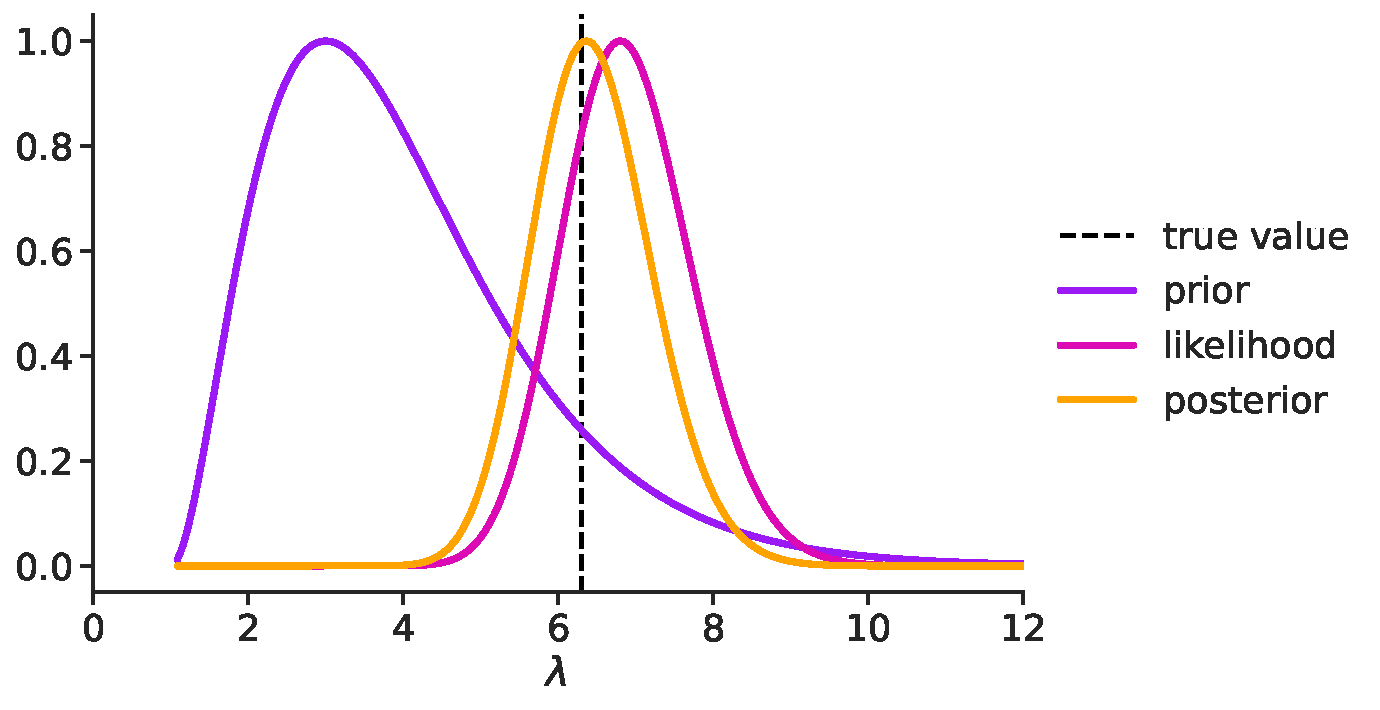
\includegraphics[width=0.9\linewidth]{figures/ch2/poisson/pdf_0.pdf}
    \caption{Analytic prior, likelihood and posterior of a Poisson rate parameter $\lambda$, obtained from $N=10$ data and a gamma prior. The distributions are not normalized.}
    \label{fig:poisexact}
\end{figure}

Consider a simple model with one parameter and a closed formula for the posterior. Given $N$ samples $y$ drawn from a
Poisson distribution, the objective is to infer its rate $\lambda$. 
Since the parameter $\lambda$ is defined as continuous and positive, this constraint can be enforced in the model by using a prior distribution that is nonzero only for positive values. A common choice for this case is the Gamma distribution, which paired with the poissonian likelihood defines the following model:
\begin{eqnarray}
    &{\mathrm{Gamma}}(\lambda|\alpha,\beta)={\frac{\beta^{\alpha}}{\Gamma(\alpha)}}\,\lambda^{\alpha-1}\,{e}^{-\beta \lambda}\\
    &\text{Poisson}(y\mid\lambda) = \prod_{i=1}^N \frac{\lambda^{y_i}}{y_i!}e^{-y_i}
\end{eqnarray}
A widespread alternative notation for statistical models, which will be used for the rest of the thesis, consists in
writing them as a series of sampling statements, denoted by $\sim$. In each sampling statement, the variable on the
left is declared as being distributed according to the function on the right-hand-side. In this case, the model can be
rewritten as:
\begin{eqnarray}
    \lambda \sim \text{Gamma}(\alpha, \beta) \\
    y \sim \text{Poisson}(\lambda)
\end{eqnarray}
It is essential to clarify that this notation only defines the functions that are used to compute the posterior. The
posterior itself will almost always be a different distribution from that used in the sampling statement of the corresponding
parameter.

While the Gamma distribution may seem as an unusual choice, in this case it allows obtaining a simple analytic expression for
the posterior. In fact, it can be shown that applying Bayes' theorem to a Gamma prior and a Poisson likelihood results
in another Gamma distribution. This property manifests for many other pairs of common distributions, known as conjugate
priors, for which the prior and the posterior belong to the same functional family \cite{diaconis1979conjugate}. For this example, the exact posterior is given by:
\begin{equation}
    p(\lambda\mid y, \alpha, \beta) = \text{Gamma}(\lambda\mid \alpha + N \overline{y},\, \beta + N)
    \label{eq:gamma_post}
\end{equation}
Where $\overline{y}$ is the mean of the data. The prior, likelihood and posterior are plotted in Fig \ref{fig:poisexact},
showing how the three components interact and provide results converging to the true rate parameter. With the analytical solution, it can be seen how the information provided by data overcomes the arbitrariness of prior choice. In fact, the mean and standard deviation of the posterior are equal to:
\begin{equation}
    \mu_{\text{post}}=\frac{\alpha + N \overline{y}}{\beta + N},\qquad     \sigma_{\text{post}}=\frac{\sqrt{\alpha + N \overline{y}}}{\beta + N},
\end{equation}
Which converge to the usual frequentist estimates $\mu=\overline{y}$ and $\sigma_\mu=\sqrt{\overline{y}/N}$ in the limit of large $N$.


\section{Markov Chain Monte Carlo}

\subsection{Integrals in high-dimensional spaces}
The current renovated interest in bayesian methods is somewhat unusual,
since bayesian statistics trace their roots in the centuries-old ideas of the founding
fathers of probability, the likes of Bernoulli, Bayes, Laplace and Gauss, while frequentists methods have become
predominant in the 20th century.
The contemporary rediscovery of Bayesian statistics is partly due to the fact that only in the last decades the necessary computational tools to tackle complex problems with a fully bayesian approach have become sufficiently powerful.
While working with a full probability density certainly is more difficult than with point estimates, the difficulty of
carrying out bayesian inference in practice may seem strange given the simple nature of Bayes' theorem, which is essentially a product of two functions.

The challenges emerge when considering models with more than one parameter. The value of the
posterior distribution can be easily computed for each point in the parameter space, but what is really needed to carry out
inference is to consider what the posterior predicts for each parameter separately. This must be done by selecting one
parameter at a time and integrating the posterior over all the others, computing what is known as the marginal
distribution of that parameter. For data $y$ and $N$ parameters $\theta_{1,\ldots N}$, the marginal posterior of the N-th parameter is given by:
\begin{equation}
    p(\theta_N \mid y)=\int d\theta_{1,\ldots N-1} p(\theta_{1,\ldots N}\mid y)
    \label{eq:marginal}
\end{equation}
For each parameter, the posterior mean, credibility intervals and all other quantities that are used for reporting and further inference must be obtained from the corresponding marginal posterior.
Since in modern applications statistical models can easily contaicolorsn thousands of parameters, it becomes essential to
address the feasibility of these integrals. 

Efficient computational methods seek to avoid unnecessary regions of parameter space which provide minimal contributions to the desired result.
An intuitive approach would be to focus on regions where the integrand is maximized, corresponding to those around the mode of
the distribution that must be marginalized. However, this overlooks a critical detail: the accumulation of integral
values requires consideration of both the probability density and the volume of parameter space.
This is due to the fact that a distribution alone only defines the density of probability for each point. The actual
probability of an event occurring in a specific range of values is given by the integral of the distribution over that range.

One of the characteristic properties of high-dimensional spaces is that there is much more volume outside any given neighborhood than inside of it.
This means that for probability distributions defined over spaces with many dimensions the region containing the mode, while still featuring the highest probability density, is contained in a very small volume.
As the number of dimensions increases, the region containing most of the probability shifts away from the mode, since the decreasing probability density is balanced with exponentially larger volume in the integration.

With an increasing dimension of parameter space, the tension between density and volume intensifies, resulting in a
narrowing of the regions where both of them are enough substantial to contribute significantly. This phenomenon, known as the concentration of measure, explains the inefficiency of brute force methods for computing integrals in many dimensions. For example, naive quadrature requires an exponentially growing number of evaluations as the dimensionality increases, yet is unlikely to intersect the narrow useful region that contributes significantly. 

%To provide an intuitive interpretation of this phenomenon, consider a multivariate standard normal with $N$ dimensions and centered on 0. In the N-dimensional space, the distance of any $N$-dimensional sample $x$ from the mode is  $\sqrt{\sum x^2}$. It becomes evident that the mean of this distance can only increase as dimensions are added because all contributions must be positive. In fact, the sum of squared standard normal variables is distributed as $\chi^2(N)$, and its square root follows a chi-distribution with N degrees of freedom. For large $N$, the mean $\mu$ of a $\chi(N)$ distribution is approximately $\sqrt{N-\frac{1}{2}} $, while its variance $N-\mu^2$ approaches $\frac{1}{2}$. This means that while the total mean distance of the samples from the mode increases indefinitely with dimensionality, their variance asymptotically reaches a fixed value. Consequently, the typical set becomes singular relative to the rest of the parameter space, as shown in figmiaoo.




\subsection{The algorithm}
Markov Chain Monte Carlo (MCMC) methods are a class of algorithms designed to probabilistically approximate integrals
and expectations by generating samples from the distribution that must be integrated \cite{geyer2011introduction}. A Markov chain is a sequence of
random variables $\{x_i\}$, where the probability of obtaining the next value is explicitly dependent only on the
current one. This conditional probability density is referred to as a Markov transition, denoted as $\mathbb{T}(x_{i+1} \mid x_{i})$. Starting from an initial point $x_1$, the sequence is constructed by iteratively applying this transition, each time sampling a new value that updates the position of the chain. The probability of reaching the N-th point in the sequence is given by:

\begin{equation}
    p(x_N) = p(x_1) \prod_{i=1}^{N-1} \mathbb{T}(x_{i+1} \mid x_{i})
\end{equation}
It is important to clarify that each $x_i$ is not an additional dimension or parameter, but that it is simply a point
in a possibly multi-dimensional space.

In a general Markov chain, the sequence simply explores parameter space without any particular utility for computing expectations. However, something remarkable occurs when the Markov transition preserves a certain target distribution $p(x)$, as expressed by the equation:

\begin{equation}
    p(x_{i+1}) = \int dx_{i} \mathbb{T}(x_{i+1} \mid x_{i})p(x_{i}) 
\end{equation}

This preservation property states that new samples generated by applying $\mathbb{T}$ to a series of samples from $p$
are still distributed according to $p$. Conversely, this means that the points in a Markov chain generated by this
transition will eventually be approximately distributed as $p$, regardless of the initial value. Given sufficient time,
the samples produced by the Markov chain enable to compute unbiased estimates for the expectation value of any function
$f$ over $p$. This is done by averaging $f$ over the Monte Carlo samples:

\begin{equation}
    \hat{f}_N = \frac{1}{N} \sum_{i=1}^N f(x_i)
\end{equation}

As the number of samples $N$ approaches infinity, these estimates converge to the true expectation $\mathbb{E}_p[f]$. 
A central aspect of this approach is the fact that expectations over the marginal distribution of a parameter are obtained simply by considering all the samples according to that parameter and discarding the dependence from the others, allowing to approximate the problematic integrals of Eq \ref{eq:marginal} in an efficient way.

In practice, achieving this asymptotic behavior is often infeasible due to limited computational resources. Thus, it is more pragmatic to consider the behavior of a Markov chain for a finite number of samples, which can be divided into three distinct phases when exploring the target distribution.
First, the chain converges from its starting position towards the region containing most of the probability defined by
the distribution $p$, leading to highly biased estimators. Second, immediately after entering that region, the exploration becomes much more efficient, rapidly reducing bias. Finally, the chain continues to refine its exploration of the distribution, resulting in slower but ongoing improvements in estimator precision. During this third phase, the estimators follow a central limit theorem:

\begin{eqnarray}
  \hat{f}^{\text{MCMC}}_N &\sim& \text{Normal} (\mathbb{E}_p[f], \sigma_{\text{MCMC}})\\
  \sigma_{\text{MCMC}} &=& \sqrt{\frac{\text{Var}_p[f]}{\text{ESS(N)}}}
\end{eqnarray}

Here, ESS (Effective Sample Size) quantifies the number of independent samples from $p$ needed to produce an equivalent
estimate. Considering that perfectly random samples must be uncorrelated, the ESS is given by the number of MCMC samples adjusted for their autocorrelation.

\subsection{Metropolis-Hastings MCMC}

The various implementations of MCMC differ in their ways to construct a transition $\mathbb T$ that ensures the
preservation property for any distribution. One commonly used method is the Metropolis-Hastings algorithm \cite{chib1995understanding}, which generates transitions through a two-step process involving proposal and acceptance. The proposal can be any stochastic perturbation of the initial state $q(x_{i+1}\mid x_{i})$. The most common choice is a gaussian distribution
\begin{equation}
  q(x_{i+1}\mid x_{i})=\text{Normal} (x_{i+1}\mid x_{i}, \sigma)
\end{equation}
On the other hand, the acceptance step is used to correct any proposals that stray too far away from the target distribution by rejecting them. The probability of accepting any proposal is given by
\begin{equation}
    a(x_{i+1}\mid x_i)=\operatorname*{min}\biggl(1,{\frac{p(x_{i+1})\,q(x_{i+1}\mid x_i)}{p(x_i)\,q(x_i\mid x_{i+1})}}\biggr)\,
\end{equation}
If the proposal is simmetric, such as in the case of the normal distribution, the acceptance probability reduces to:
\begin{equation}
    a(x_{i+1}\mid x_i)=\min \left( 1, \frac{p(x_{i+1})}{p(x_i)} \right)
\end{equation}
In contrast, asymmetric proposals find application in variants of the Metropolis-Hastings algorithm, such as Gibbs
sampling, which is widely used in statistical practice and implemented in software like JAGS \cite{plummer2003jags} and BUGS \cite{lunn2000winbugs}.

It can be shown that the Markov transitions generated by the Metropolis-Hastings algorithm preserve the target
distribution because the overall probability of the resulting Markov chain being in any $x_i$ and jumping to $x_{i+1}$ is the same as that
of it being in $x_{i+1}$
and jumping to $x_i$. This property, known as reversibility, is sufficient but not necessary to ensure the
preservation of the distribution. 

While Metropolis MCMC remains popular in many applications, its performance tends to degrade as the dimensionality of
the target distribution increases. The primary reason for this is again the concentration of measure. As the dimensionality grows,
the volume outside of the region useful for integrating the target distribution expands exponentially. Consequently, a
significant portion of proposals consists of points with extreme values in at least one dimension, leading to high rejection rates. Because of this, the Markov chain explores the distribution at an exceedingly slow pace.

In a broader context, challenges arise in all MCMC techniques when dealing with complex distributions, since the
effectiveness of a Markov transition heavily depends on their geometry. For example, in scenarios where the geometry
features narrow corners and high-curvature regions, standard Markov transitions may struggle to explore effectively,
resulting in biased estimations due to incomplete exploration. Markov chains can become trapped near the boundaries of
problematic regions, causing oscillations in the estimates that may disrupt the convergence process if the chain is
terminated prematurely. The concept of geometric ergodicity offers a formal guarantee of ideal behavior, including the
Central Limit Theorem for MCMC estimators \cite{jarner2000geometric}. However, verifying this property theoretically is challenging for all but the simplest cases, and in practice a set of empirical diagnostics is usually employed to assess the robustness of MCMC results.

\subsection{Hamiltonian Monte Carlo}
The Hamiltonian Monte Carlo (HMC) algorithm overcomes the limits of Metropolis-Hastings MCMC by generating efficient
proposals that consider the geometry of the target distribution \cite{betancourt2017conceptual}. To do so, it simulates a physical system akin to a frictionless particle subject to a potential given by the target log-likelihood function, denoted as $p(\theta)$.

In the HMC framework, each parameter of interest $\theta$ is paired with its canonical conjugate variable, denoted as $\rho$. These pairs define a joint canonical distribution $p(\theta,\rho) = p(\rho|\theta) \cdot p(\theta)$. The log-likelihood of this joint density is introduced as an artificial Hamiltonian:

\begin{align}
H(\theta,\rho) &= -\log p(\rho|\theta) - \log p(\theta) \\
&\equiv K(\rho,\theta) + V(\theta)
\end{align}

In each HMC transition, an initial momentum value is randomly drawn, initiating a trajectory which is computed through the integration of Hamilton's equations:

\begin{eqnarray}
  \frac{d\theta}{dt}& =& +\frac{\partial H}{\partial \rho} = \frac{\partial K}{\partial \rho} \\
  \frac{d\rho}{dt}& = &-\frac{\partial H}{\partial \theta} = -\frac{\partial K}{\partial \theta} - \frac{\partial V}{\partial \theta}
\end{eqnarray}

This trajectory is calculated for a fixed time, and a new point in parameter space is sampled at its endpoint, which
then serves as the starting position for the next trajectory. In this way, while the computational cost of
producing each HMC sample is quite high, the samples are guaranteed to preserve the geometry of the target distribution and feature low autocorrelation, due to the potential for the initial and final points of the trajectories to be widely separated.  The numerical integration of the trajectory employs the leapfrog integrator, which discretizes the simulation into $L$ small time intervals  $\epsilon$, interleaving half-step updates for momentum with full-step updates for position:

\begin{eqnarray}
\rho_{n+\frac{1}{2}} &\leftarrow &\rho_{n} - \frac{\epsilon}{2} \frac{\partial V}{\partial \theta}(\theta_{n}) \\
\theta_{n+1} &\leftarrow &\theta_n + \epsilon \rho_{n + \frac{1}{2}} \\
\rho_{n+1} &\leftarrow &\rho_{n+\frac{1}{2}} - \frac{\epsilon}{2} \frac{\partial V}{\partial \theta}(\theta_{n+1})
\end{eqnarray}

If numerical integration were perfect, every proposed transition would be accepted. However, the leapfrog integrator introduces a global error of order $\epsilon^2$. Fortunately, errors in numerical integration can be corrected by ensuring that the energy remains constant throughout the trajectory. This is accomplished through a Metropolis acceptance step with probability:

\begin{equation}
a(\theta_{L},-\rho_{L}|\theta_{0},\rho_{0}) = \min (1, \exp(H(-\rho_L,\theta_L)-H(\rho_0, \theta_0)))
\end{equation}

Where the inversion of the final momentum, denoted as $-\rho_L$, is required to maintain the reversibility of the
transition. While HMC is highly efficient, and proposals of well-conditioned Markov chains commonly reach acceptance rates higher than 90\%, if the simulation is not able to discretize the trajectories with sufficient precision the initial and final values of the Hamiltonian differ too much from each other, indicating that the algorithm is not correctly sampling from the distribution and leading to what are known as divergent transitions. 

To provide satisfying results, the basic version of HMC requires optimization in two key aspects:

\begin{description}
\item[Choice of Kinetic Energy:] In many applications, the momenta are sampled independently from the parameters using a
  multivariate normal distribution, $p(\rho|\theta) = p(\rho) = \text{Normal}(0, M)$, where $M$ is the Euclidean metric
  of the parameter space given by the correlation matrix between parameters. More sophisticated methods such as
  Riemannian HMC use a metric explicitly dependent on the position in parameter space.
\item[Leapfrog integrator's parameters:] while the step lenght $\epsilon$ defines the precision with which the
  trajectory is simulated, and thus the ability of properly describing the distribution, the combination of step lenght and number $\epsilon L$ determines the balance between producing long and very costly transitions or short trajectories that generate highly correlated samples.
\end{description}

Apart from the usual difficulties in exploring complex distributions with very high curvature regions, another limitation of HMC lies in its reliance on gradient-based methods, making it unsuitable for evaluating models with discrete parameters. Nevertheless, HMC can still be applied to many apparently discrete models by finding suitable reparametrizations and alternative formulations.

\subsection{No U-turn sampler and Stan}

The No-U-Turn Sampler (NUTS) is an extension of the Hamiltonian Monte Carlo (HMC) algorithm that enhances its
performance by automatically adjusting its parameters. In this implementation, the number of steps taken varies for each
transition. Instead of sequentially adding the steps of the leapfrog integrator, they are accumulated within a binary
tree of possible trajectories until one of them either turns back on itself (referred to as a "U-turn") or diverges,
with the maximum number of doublings in this tree structure being known as the tree depth. Intuitively, a U-turn occurs
when the momenta at the two extremes of the trajectory point towards each other. This implies that further extending the
trajectory would bring the initial and final points closer, resulting in a less efficient proposal due to the fact that
closer samples are more correlated.

NUTS uses an initial set of samples to achieve convergence and determine the optimal step size and metric. This phase is referred to as the "warm-up" phase. The tuned parameters are then employed for all subsequent sampling iterations. The adaptation process involves targeting a fixed acceptance rate, which is set by the user. Typically, this target acceptance rate falls between 0.6 and 0.9. Higher values lead to smaller steps and more precise trajectories but result in slower sampling due to the increased number of steps required.

Throughout this thesis, inference will be conducted using Stan \cite{carpenter2017stan}, a probabilistic programming language that implements the NUTS variation of HMC and other inference algorithms. Stan is primarily written in C++, and its language closely resembles C++. A Stan program is structured into a sequence of blocks, which are divided in seven different types:

\begin{description}
\item[Functions:] Contains a list of functions declarations and definitions to be used in the following code.

\item[Data:] The Data block is used to declare input variables. These data variables remain untransformed, and statements other than declarations are not allowed in this block.

\item[Transformed Data:] In this block, variables that do not need to change during program execution are declared. Unlike the Data Block, there's no reading from external sources; instead, it involves additional declarations and transformations of data variables. The statements in this block are executed once per chain after data is read.

\item[Parameters:] This block is used for declaring the parameters to be sampled by Stan’s NUTS implementation. These
  parameters cannot be directly assigned values and are updated at every leapfrog step of the sampler.

\item[Transformed Parameters:] This block contains additional declarations of parameters derived from the original ones
  or mixed with data variables. This block can be used to implement alternative and more efficient reparametrizations of the model.

\item[Model:] The Model block implements the actual probability model as a series of sampling statements targeting the
  parameters or the data, with all the statements concurring to define the target log-distribution that will be sampled. If priors are not explicitly defined for a certain parameter, a uniform  prior over its whole allowed range is automatically assigned to it.

\item[Generated Quantities:]This block is used for computations that do not affect the sampled parameters. It is executed each time after a sample has been generated and variables declared here are printed as part of the output. This block finds applications in generating predictions for new data, calculating event probabilities, saving the likelihood of each datapoint for model comparison and many other uses.

\end{description}

A Stan program is created by compiling a .stan model. The stanc compiler converts this model to C++ and then to an executable. The compiler and the execution of the HMC algorithm can be accessed through interfaces in various programming languages. While some interfaces provide access only to the compiler and the inference algorithms (e.g., CmdStan's command line interface), others offer additional functionality through languages like R, Python, or Julia. Among these, RStan is the most feature-rich library at the moment.
While libraries such as Rstanarm for R simplify the implementation of Stan models with pre-built functions, writing code directly in Stan allows for a deeper understanding of its inner workings and the ability to leverage its full potential. This is particularly valuable in physics applications, where models often require the implementation of specific functions and do not rely on standard classes such as linear regression.
In this thesis, all models are written directly in Stan and executed using CmdStanPy, a lightweight Python wrapper for the command line interface. Additional functions have been implemented in a Python package called "baynes", which utilizes data analysis libraries such as Seaborn and ArviZ to organize the models, plot useful graphs and aid in the execution of standard analysis routines.

\subsection{Model fitting with Stan}
Let's start by fitting with HMC the simple Poisson model of Sec \ref{sec:example}.
Here is the full implementation in Stan:
\begin{lstlisting}[language=Stan]
data {
  int<lower=0> N;
  array[N] int y;
  real alpha;
  real beta;
  int<lower=0, upper=1> prior;
}

parameters {
  real<lower=0> lambda;
}

model {
  lambda ~ gamma(alpha, beta);
  if (prior == 0){
    y ~ poisson(lambda);
  }
}
\end{lstlisting}
As can be seen, Stan allows to add constraints to the variables declarations, including parameters, which will be automatically enforced during sampling. The additional flag variable "prior" is used to switch between sampling only from the prior or from the posterior distribution when running the model without the need to recompile it.
The priors could also be checked using one of the many methods of numpy.random, scipy.stats or one of the rng functions of Stan, which would provide perfectly uncorrelated samples in less time.
Using either method is strictly a personal choice. In the examples of this thesis it has been preferred the ease of not
needing to rewrite part of the model in another language or recompile a nearly identical Stan program. Moreover,
checking if HMC struggles already when sampling from the priors allows to identify whether they are grossly
misspecified or if there are other possible problems in the implementation of the model.


\begin{figure}[t]
    \begin{subfigure}[b]{0.45\linewidth}
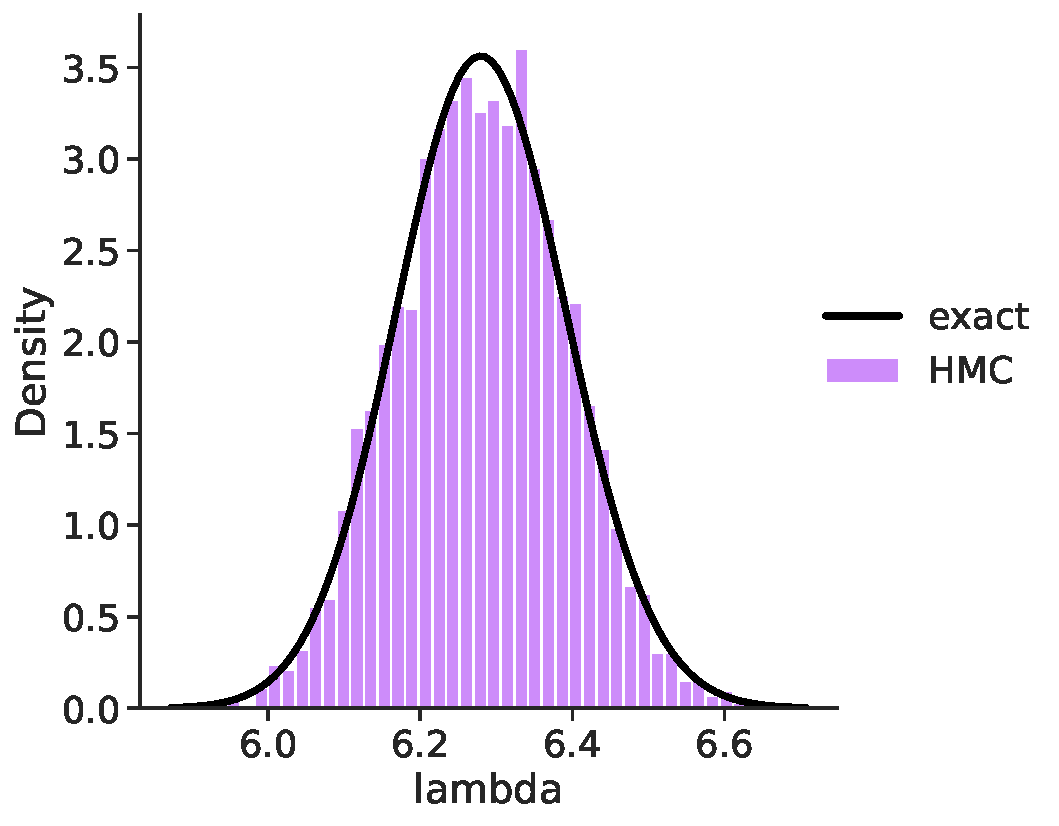
\includegraphics[width=\linewidth]{figures/ch2/poisson/plot_3.pdf}
\caption{}
\end{subfigure}
%\hfill
\begin{subfigure}[b]{0.5\linewidth}
    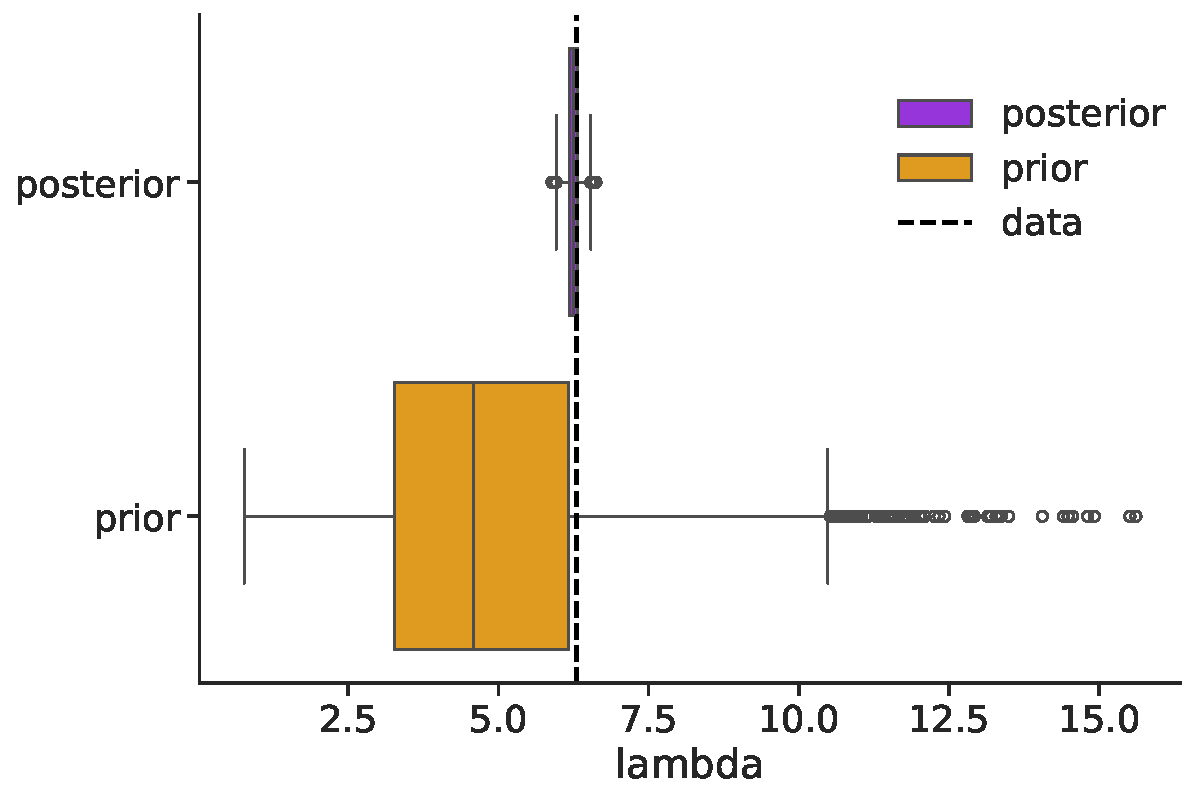
\includegraphics[width=\linewidth]{figures/ch2/poisson/cat_plot_0.pdf}
\caption{}
\end{subfigure}
\caption{Histogram of the HMC samples and analytical posterior for the rate parameter of a Poisson model (a). Boxplots of the prior and posterior HMC samples (b). } 
\label{fig:poispost}
\end{figure}

For a practical example, $N=100$ data points are generated from a Poisson with $\lambda=6.3$. Since the gamma distribution has mean $\mu=\frac{\alpha}{\beta}$ and variance $\sigma^2=\frac{\alpha}{\beta^2}$, $\alpha=5$ and $\beta=1$ are chosen to obtain a prior centered on 5 and spread between 0 and 10.
The model is compiled with CmdStanPy and fitted by running 4 chains with 500 warmup iterations and 1000 sampling
iterations each. The number of samples can be chosen depending on the precision with which the posterior estimates need
to be computed, especially for tail quantities, but this should be done considering not the raw number of iterations but the final effective sample size.

\begin{lstlisting}[language=Python]
N=100
lambda_true = 6.3
events = np.random.poisson(lambda_true, N)
data = {'N': len(events), 'y': events,
        'alpha': 5, 'beta': 1, 'prior': 0}

model = CmdStanModel(stan_file='poisson.stan')
fit = model.sample(data, chains=4,
                   iter_warmup=500,
                   iter_sampling=1000)
\end{lstlisting}



The fit results are shown in Fig \ref{fig:poispost}. The plot on the left shows an histogram of all the posterior
samples
after warmup and the exact posterior of Eq \ref{eq:gamma_post}. The two distributions provide identical estimates of mean,
standard deviation and quantiles to the third decimal place. The second plot compares the posterior and prior
distributions using boxplots, showing how much the posterior shirnks towards the true value of $\lambda$. Boxplots are a common visualization method to summarize 1-D distributions using their quartiles. The central box is given by the 25\%, median and 75\% quantiles, while the external lines extend for 1.5 quartile ranges or up to the first and last data points. Eventual outliers are plotted as single points. 

\section{Controlling the MCMC algorithm}

\subsection{HMC diagnostics}
This section will describe various diagnostics and techniques that can be applied to check for the proper working of a
Markov Chain Monte Carlo algorithm or to improve its efficiency.

While properly conditioned Markov chains are theoretically guaranteed to converge to the target distribution, this does not mean that they may do so in a reasonable time. 
The simplest way to assess potential issues with the Markov chain consists of examining the samples as a function of
each iteration, as depicted in Figure \ref{fig:pois_trace}. This graphical representation, known as a traceplot, helps
to determine whether all chains converge to the same parameter region and if they stabilize after the warm-up period.
In the case of the simple Poisson model the chains converge almost instantly, as shown in the inset which focuses on the first 50 iterations.

While traceplots are useful, they alone cannot reliably confirm the correct behavior of the Markov chains. Ensuring
their efficiency and accuracy requires various heuristics and tests since proving geometric ergodicity directly is
challenging. Fortunately, Hamiltonian Monte Carlo (HMC) offers numerous methods to assess its performance. The
"diagnose" function, accessible through every Stan interface, provides a comprehensive set of diagnostics to identify potential problems:
\vfill
\begin{figure}[t]
    \centering
    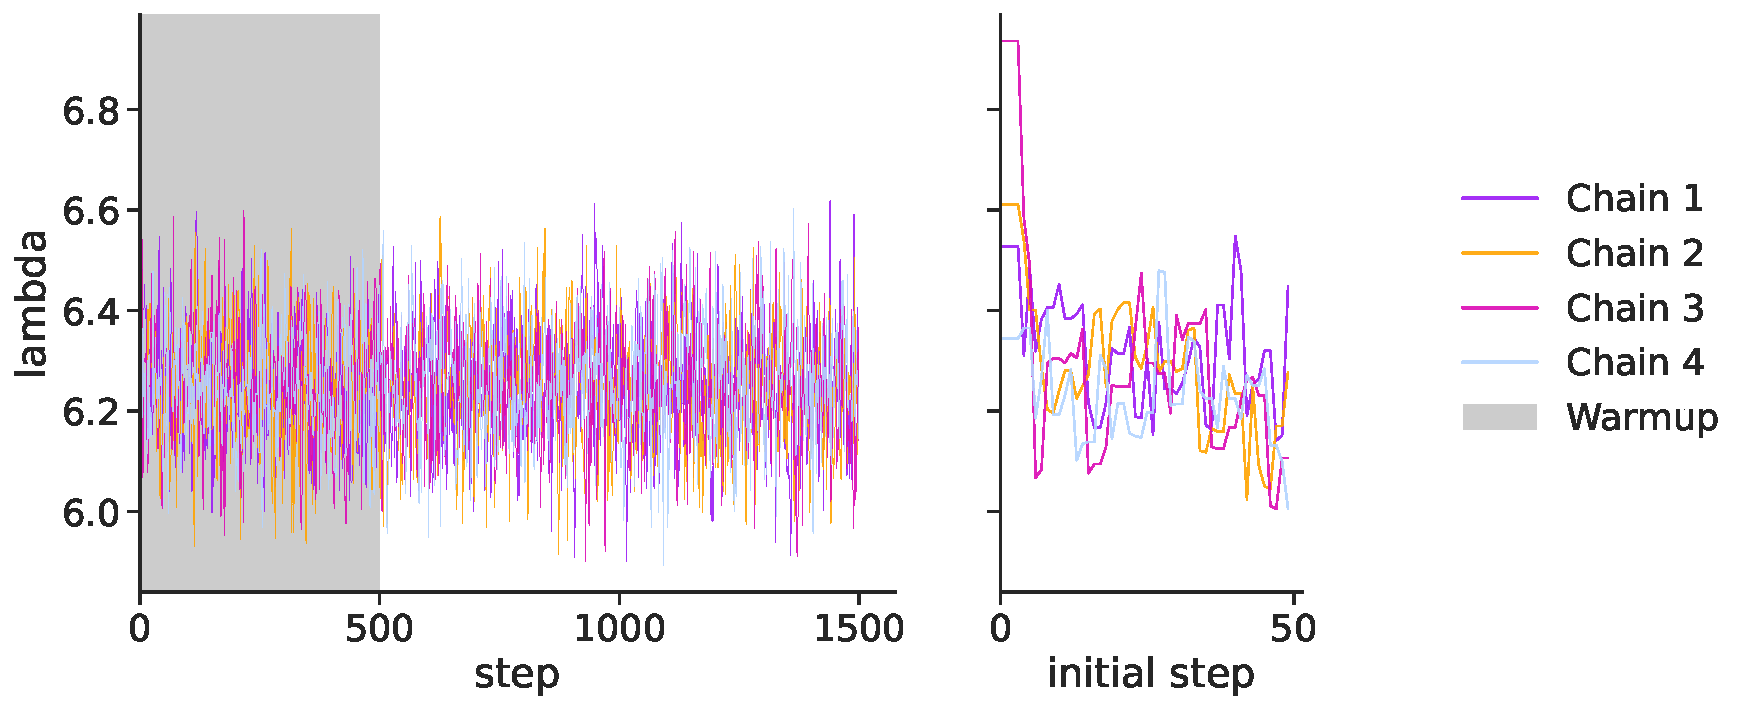
\includegraphics[width=0.9\linewidth]{figures/ch2/poisson/convergence_plot_0.pdf}
    \caption{Traceplot of the HMC chains for the rate parameter $\lambda$ of the Poisson model. The right-side plot shows how the chains rapidly converge to the posterior distributions in the first warmup iterations.}
    \label{fig:pois_trace}
\end{figure}
\vfill
\begin{description}
\item[Divergent Transitions after Warmup:] These occur when the leapfrog integrator fails to accurately approximate the
  trajectory, leading to the energy not being conserved. This issue arises when the tuned step size is inappropriate for posterior regions with complex geometry, such as narrow corners. While samples from divergent transitions are discarded and do not affect the final estimates, they indicate that the sampler struggles to explore the posterior, potentially yielding biased estimates.
\item[Maximum Treedepth Exceeded:] To prevent exceedingly long computation times, the number of branches generated by the No-U-Turn Sampler (NUTS) during each transition is capped. Hitting this limit many times typically does not introduce bias, but it signals an efficiency problem.

\item[Low E-BFMI Values:] Low values indicate inefficient exploration and high correlation among the Markov chain draws.
  This score is constructed considering that the canonical distribution $p(\rho, \theta)$ can be expressed in terms of
  energy $E$ and coordinates on an energy level $\phi$ through the microcanonical decomposition $p(E, \phi) p(E)$, with
  $p(E)$ being the marginal energy distribution \cite{betancourt2016diagnosing}. Efficient exploration requires the distribution of energies defined by momentum resampling $p(E\mid \theta)$ to closely resemble $p(E)$. The E-BFMI (Energy Bayesian Fraction of Missing Information) is the ratio of the variances of these two distributions.

\item[Low Effective Sample Size:] A low effective sample size indicates that the Markov chains are producing highly
  correlated samples, often due to very short transitions. Achieving accurate estimates, especially for extreme values,
  might require running the chain for a longer duration.

\item[High Split-$\hat{R}$:] A high Split-$\hat{R}$ score suggests that different chains have not converged by the end
  of the warm-up phase or have converged to different modes of the posterior and are not able to mix properly. The
  Split-$\hat{R}$ score is constructed by comparing the variance of all the samples together with that of each
  half-chain \cite{vehtari2021rank}.
\end{description}

To effectively diagnose sampling problems, it is highly recommended to run multiple chains from different starting
points, with a common minimum recommendation of four chains. In addition to using the $\hat{R}$ score, running multiple
chains increases the likelihood of identifying multimodality of the posterior, poor adaptation, or mixing issues.



\subsection{Reparametrization}\label{sec:repar}
As described previoulsy, Markov chain algorithms tend to perform badly when the distribution from which they extract samples has a complex shape, especially when featuring narrow corners or regions with very different scales.
Difficult geometries frustrate the HMC algorithm, leading to
slower computation times, lower effective sample size and divergent transitions. 
This problem can easily arise in models where some parameters depend explicitly from other parameters, such as those that will be described in the last section of this chapter.
A simple example is known as the
"Devil's funnel", which doesn't even require to perform inference over data but just to sample two parameters according to
the following distribution:

\begin{eqnarray}
  y&\sim&\mathrm{normal}(0,3)\\
  x &\sim&\mathrm{normal}(0,\exp(y))
\end{eqnarray}

Its fundamental characteristic is that the scale of one parameter is strongly dependent on the value of the other. Since
in HMC the optimal step size is fixed after warmup, this extreme correlation induces divergent transitions when trying to
sample in the region where the funnel becomes narrower. At the same time, selecting a very short stepsize would mean not being able to efficiently explore the broader part of the distribution.

\begin{figure}[t]
\begin{subfigure}[b]{0.31\linewidth}
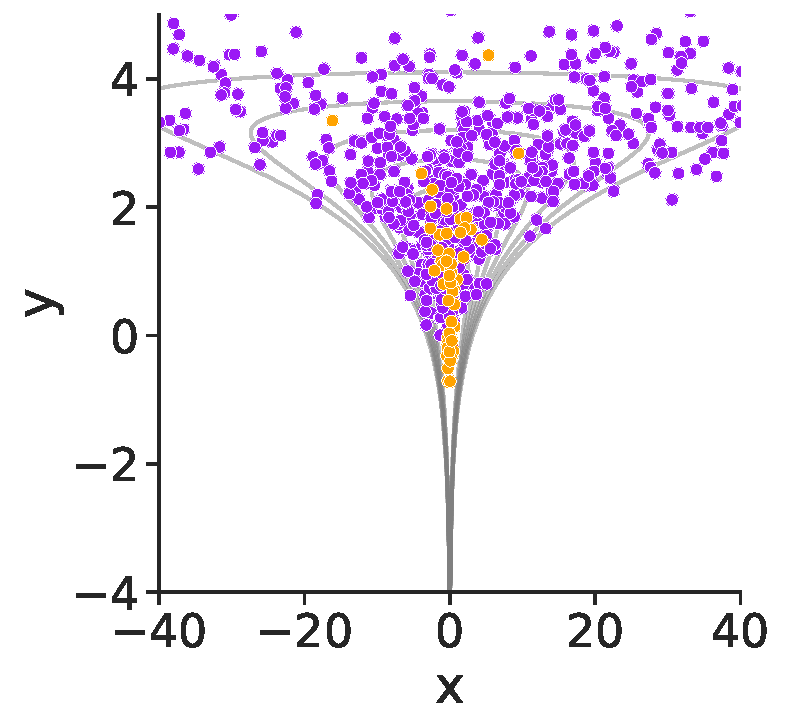
\includegraphics[width=\linewidth]{figures/ch2/poisson/funnel_0.pdf}
\caption{}
\end{subfigure}
\hfill
\begin{subfigure}[b]{0.31\linewidth}
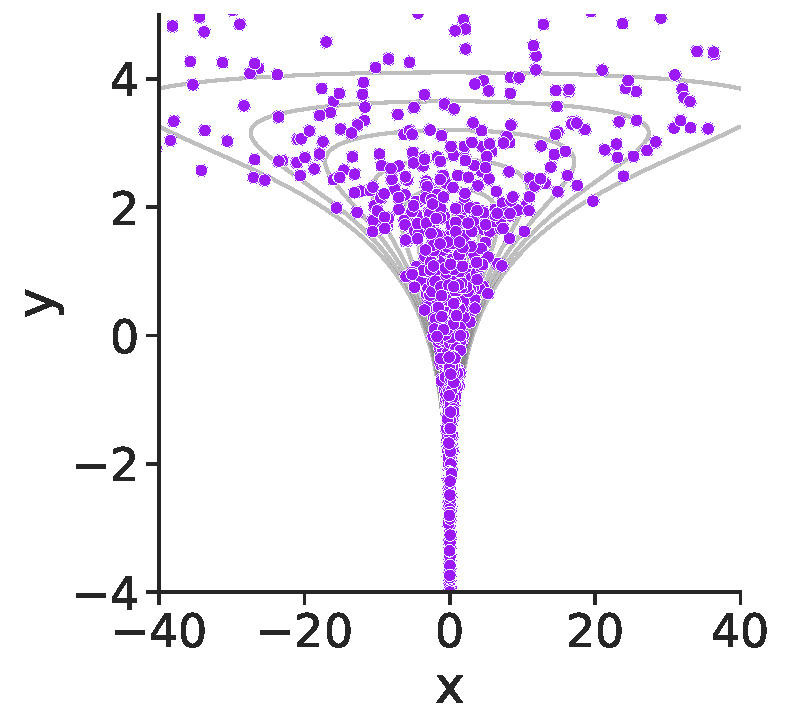
\includegraphics[width=\linewidth]{figures/ch2/poisson/funnel_1.pdf}
\caption{}
\end{subfigure}
\hfill
\begin{subfigure}[b]{0.31\linewidth}
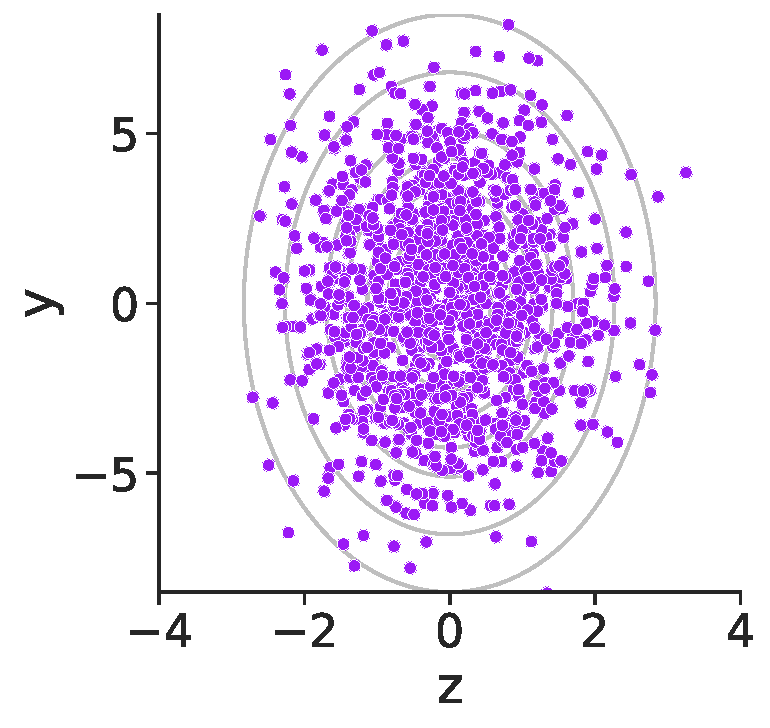
\includegraphics[width=\linewidth]{figures/ch2/poisson/funnel_2.pdf}
\caption{}
\end{subfigure}
\caption{Posterior samples for the funnel model. The centered parameterization induces divergent transitions (orange) and is
not able to explore the full distribution (a). On the other hand, the non-centered parameterization features no
divergences and is able to reach inside the funnel (b). This is because Stan is actually sampling the parameters $y$ and $z$
from normal distributions and then transforming them to $y$ and $x$ (c).}
\label{funnel}
\end{figure}
Manually adjusting the settings of the sampler will prove to be fruitless in many of these instances. In these cases, Stan's diagnostics will suggest to find an alternative parametrization.
Reparametrizing a model involves rewriting it in a different form that is mathematically equivalent but uses easier sampling statements for the algorithm. This is usually done by introducing some auxiliary parameters that are sampled according to simple distributions. These parameters can then be manipulated and combined with the others after each iteration to produce a more complex distribution without explicitly using it in a sampling statement. However, finding alternative reparametrizations is not always possible and depends upon the specific details of each model. 

The problematic implementation of the funnel where the distribution of $x$ is explicitly dependent on the other
parameter $y$ is known as a centered parametrization.
The alternative is a non-centered parameterization. Using an auxiliary parameter $z$ and leveraging the properties of the normal distribution, a non-centered
parameterization can place the embedded parameter $y$ out of the sampling statement for $x$:
\begin{eqnarray}
  y&\sim&\mathrm{Normal}(0,3)\\
  z&\sim&\mathrm{Normal}(0,1)\\
  x&=&z\exp(y)
\end{eqnarray}
Now the MCMC algorithm only needs to sample $y$ and $z$ from simple normal distributions with fixed standard deviations,
while $x$ can be computed after every iteration without needing to sample it directly.
The difference between the performance of these two parametrizations is shown in Fig \ref{funnel}.
This alternative form can be implemented in Stan using the transformed prameters block:

\begin{lstlisting}[language=Stan]
parameters {
  real y;
  vector z;
}
transformed parameters {
  vector x;
  x = z * exp(y);
}
model {
  y  ~ normal(0, 3);
  z ~ std_normal();
}
\end{lstlisting}




\subsection{Simulation-Based Calibration (SBC)}
While HMC diagnostics are a general set of tests that can be applied to all Markov chains produced by Stan and
reparametrization allows to greatly improve the sampling efficiency, these methods cannot perfectly guarantee the convergence of the algorithm. 
However, in some limited circumstances it is possible to check directly whether MCMC is sampling from the target distribution correctly.
The necessary condition for this to happen is that the data used to fit the model must be simulated from the model
itself. This is the core intuition of Simulation Based Calibration  \cite{talts2018validating}, which employs an interesting property of Bayesian models. 

Consider a process that first samples a parameter $\theta^{sim}$ from the prior distribution and then simulates data from this sample according to the likelihood of the model:

\begin{align}
\theta^{sim}&\sim p(\theta)\\
y^{sim}&\sim p(y\mid \theta^{sim})
\end{align}

Using the definition of conditional probability and Bayes' rule, it can be shown that $\theta^{sim}$ is also a sample from the posterior distribution for the simulated dataset $p(\theta\mid y^{sim})$. 
Now, consider using the same model to fit the simulated data with an algorithm such as HMC, obtaining $N$ samples of
the parameters distributed according to the posterior if the algorithm converges. Bewteen these posterior samples, count how many of them are less than $\theta^{sim}$, which is known as their rank statistic:

\begin{equation}
r(\theta^{sim}, (\theta_1\ldots\theta_N)) = \sum_{n=1}^N \mathbb I[\theta_n<\theta^{sim}],
\end{equation}

where $\mathbb I$ represents the indicator function. Since $\theta^{sim}$ and $\theta$ are obtained from the same
distribution if the algorithm is capable of correctly approximating the posterior, the ranks constructed by generating new values of $\theta^{sim}$, $y^{sim}$, and repeating the process should follow a uniform distribution from 0 to $N$. This holds true for ranks computed from any random variable over $\theta$, denoted as $f:\Theta\to \mathbb R$. 

%In this sense, Bayesian models are denoted as being inherently calibrated, providing appropriate coverage for their posterior intervals when the data is generated by the model itself with "true" parameters drawn from the priors.

It's important to highlight that this useful property is not true for any kind of data obtained from experiments, but
works only when the fit is repeated using data generated by the model itself with "true" parameters sampled from the priors.


However, this method allows isolating problems in the execution of the algorithm or validating another program used
to generate synthetic data through Monte Carlo simulation, ensuring consistency with the model. The other main
limitation of SBC is that it requires to repeat the fit multiple times, which can lead to impractical computation times
for complex models. In such cases, it may still be employed to validate the correct functioning of simpler models
before extending them with more parameters.

\begin{figure}[t]
\begin{subfigure}[b]{0.38\linewidth}
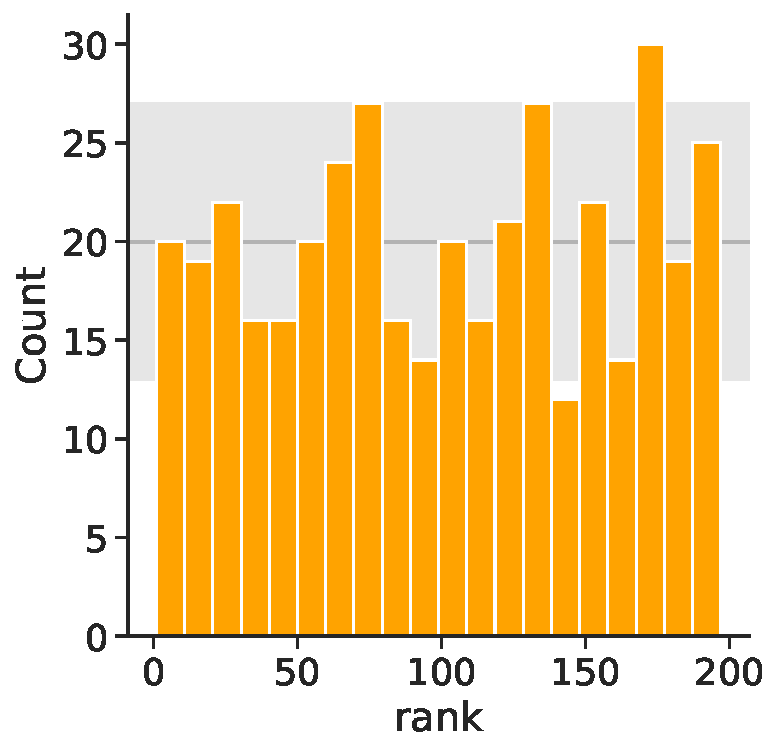
\includegraphics[width=\linewidth]{figures/ch2/poisson/SBChist_0.pdf}
\caption{}
\end{subfigure}
\hfill
\begin{subfigure}[b]{0.5\linewidth}
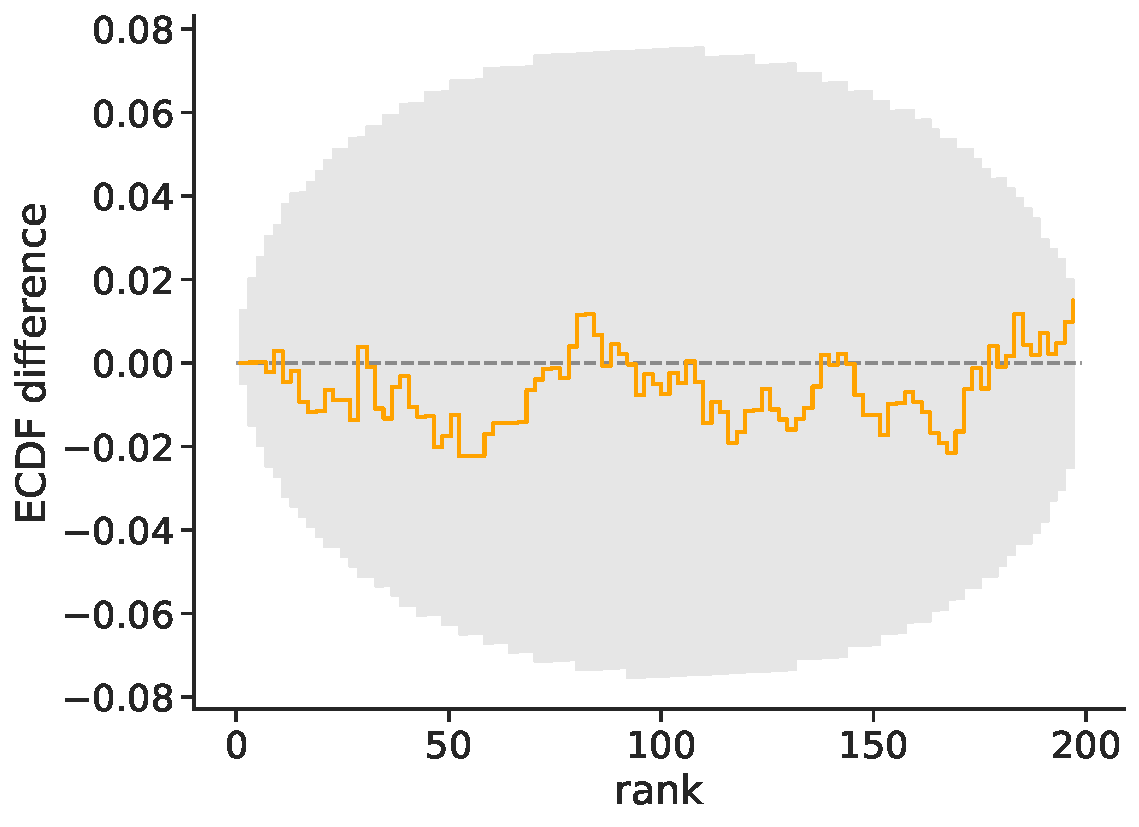
\includegraphics[width=\linewidth]{figures/ch2/poisson/SBCecdf_0.pdf}
\caption{}
\end{subfigure}
\caption{Results of SBC analysis obtained by fitting the Poisson model 1000 times, with $N=199$ samples per fit. (a) Histogram of the computed ranks for the parameter $\lambda$. (b) Difference between the ECDF of the ranks and the cumulative distribution of a uniform distribution. The grey bands represent the expected 95\% interval of possible variation assuming uniformity.}
\label{fig:poisson_SBC}
\end{figure}
SBC can be implemented within a Stan program using the transformed data block. A duplicate of the model is written in
this block, but instead of specifying a series of sampling statements, parameters and data are simulated using the
built-in RNG functions. The indicator functions, which will be accumulated into ranks, are defined within the generated
quantities block. Below is the implementation of SBC for the Poisson model, excluding the data block that is solely used
to set $\alpha$, $\beta$, and the number of data $D$:
\newpage
\begin{lstlisting}[language=Stan]
transformed data {
  real<lower = 0> lambda_sim = gamma_rng(alpha_true, beta_true);
  array[D] int<lower = 0> y = poisson_rng(rep_array(lambda_sim, D));
}
parameters {
  real<lower=0> lambda;
}
model {
  lambda ~ gamma(alpha, beta);
  y ~ poisson(lambda);
}
generated quantities {
  int<lower = 0, upper = 1> lt_lambda  = lambda < lambda_sim;
}
\end{lstlisting}
This program is executed for a total of $J$ iterations, with each iteration producing $N$ samples and a single computed
rank statistic for each parameter. %To prevent potential artifacts stemming from correlated draws, it is advisable to set $N$ close to the effective sample size ($N_{eff}$). If $N_{eff}$ is significantly lower, the chains should be sampled for a longer duration and then thinned by removing part of the samples to reduce their correlation.
The $J$ ranks can then be subjected to tests for uniformity or visually inspected using various methods. One simple
test involves accumulating the draws in a histogram with $K$ bins, where $K$ must be a divisor of $N+1$ to avoid
biases. If the expected counts per bin are sufficiently high, the distribution of counts in the histogram should follow
a chi-squared distribution with $K-1$ degrees of freedom. Alternatively, the histogram can be visualized, as shown in Figure \ref{fig:poisson_SBC} (a).

Another useful visualization method consists in plotting the difference between the empirical cumulative distribution
function (ECDF) and the expected cumulative distribution function of a uniform distribution. The ECDF at a specific
value is the proportion of samples lower than that value. The ArviZ package provides a function for plotting the
difference between the ECDF and its expected range, as demonstrated in Figure \ref{fig:poisson_SBC} (b). Visual
inspection is highly valuable, as it not only reveals whether the inference algorithm is calibrated but also how it
deviates from calibration. If the data-generating process exhibits overdispersion, underdispersion, or skewness
compared to the fitted model, these issues will be reflected in the shape of the histogram and the ECDF, which will be
significantly different from the expected range of variation.




\section{Model validation and comparison}
\subsection{Predictive checks}
The last section showed various methods for controlling the output of a MCMC algorithm and check if it has worked
properly, or to
improve its performance in order to make it correctly sample from the posterior defined by a model and the observed data.
Obtaining positive results from these procedures still does not imply anything about the ability of the model to actually describe the data, nor its usefulness. For
example, it may be extremely sensitive to priors or small variations in the underlying assumptions, or there may be
another model that generates better predictions. Different methods to address these questions will be the scope of this section.

Some of these techniques may appear unusual in the context of the standard data analysis carried out in physics, which in
many cases only requires to fit a well specified model or to
test an hypothesis. This is due to the fact that they have been developed for general applications in many other
sciences, in which it is often difficult to define a very precise theoretical model. The resulting methods are more
oriented towards model building, extending inference to a broader data analysis workflow \cite{gelman2020bayesian}. A comprehensive Bayesian workflow encompasses a sequence of interconnected
steps, from data collection and cleaning to model specification, model fitting, model expansion, and ultimately,
interpretation and decision-making. Each of these steps plays a critical role in ensuring the integrity and robustness of the analysis, aiming to capture the underlying data-generating process. 


Usually, the immediate step after controlling the convergence of a fit procedure consists in evaluating the goodness of fit.
In Bayesian data analysis, this proceeds in a way similar to Simulation Based Calibration, by simulating fake data using
the model itself \cite{gelman2013bayesian}.

When fitting a model by sampling from its posterior, the likelihood is used to compute the probability of observed data in relation to the
parameters. At the same time, in each iteration the sampled parameters define a distribution of potential new data through that same likelihood. 
Randomly sampling from the likelihood at each step of the Markov Chain generates a set of simulated data which reflects the
variability of the parameters. Notably, this simulation does not require to perform inference, but
only to sample fake data from the likelihood with an RNG function, given the parameters obtained by the Markov Chain at
that iteration.
%In this context, every Bayesian model is generative, enabling the computation of predictions by simulating data in a
%process that can be considered as "running in reverse" the likelihood.
This procedure is commonly referred to as a predictive check. Predictive checks serve as a means to evaluate whether
the model can effectively capture relevant characteristics of the data, either through visualization or by comparing
test statistics computed from the replicated datasets with those derived from the observed data. In most cases,
predictive checks are obtained from the priors or the posterior:


\begin{figure}[t]
\begin{subfigure}[b]{0.45\linewidth}
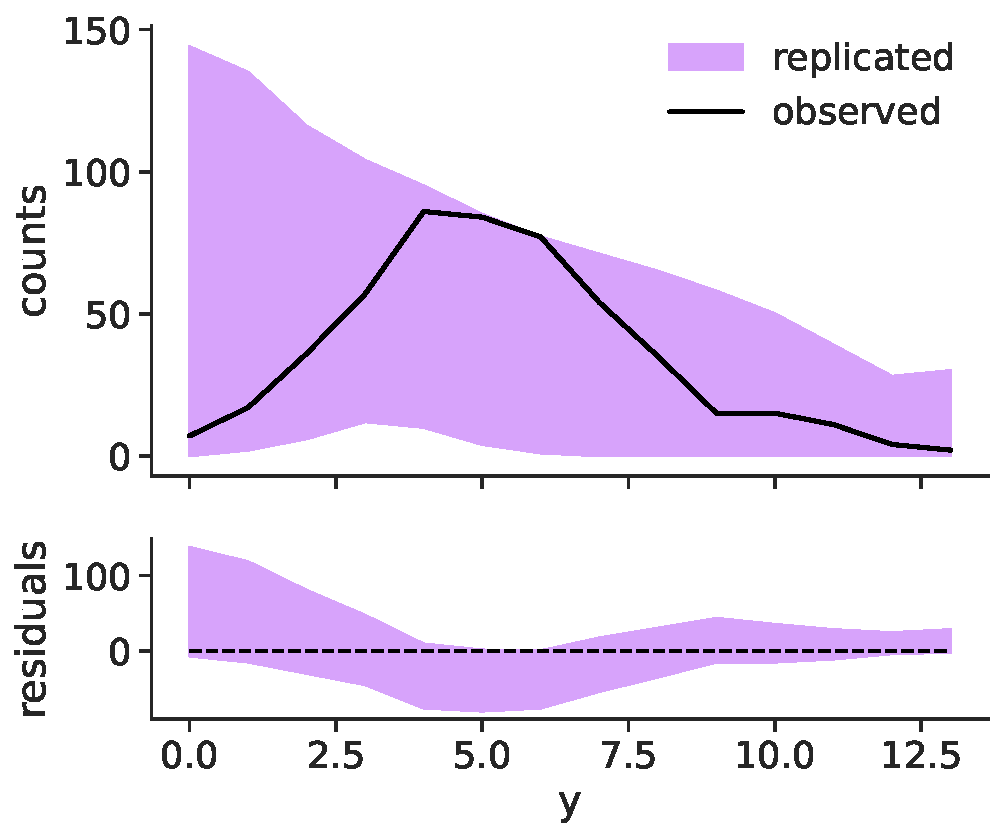
\includegraphics[width=\linewidth]{figures/ch2/poisson/predictive_check_0.pdf}
\caption{Prior Predictive Check}
\end{subfigure}
\hfill
\begin{subfigure}[b]{0.45\linewidth}
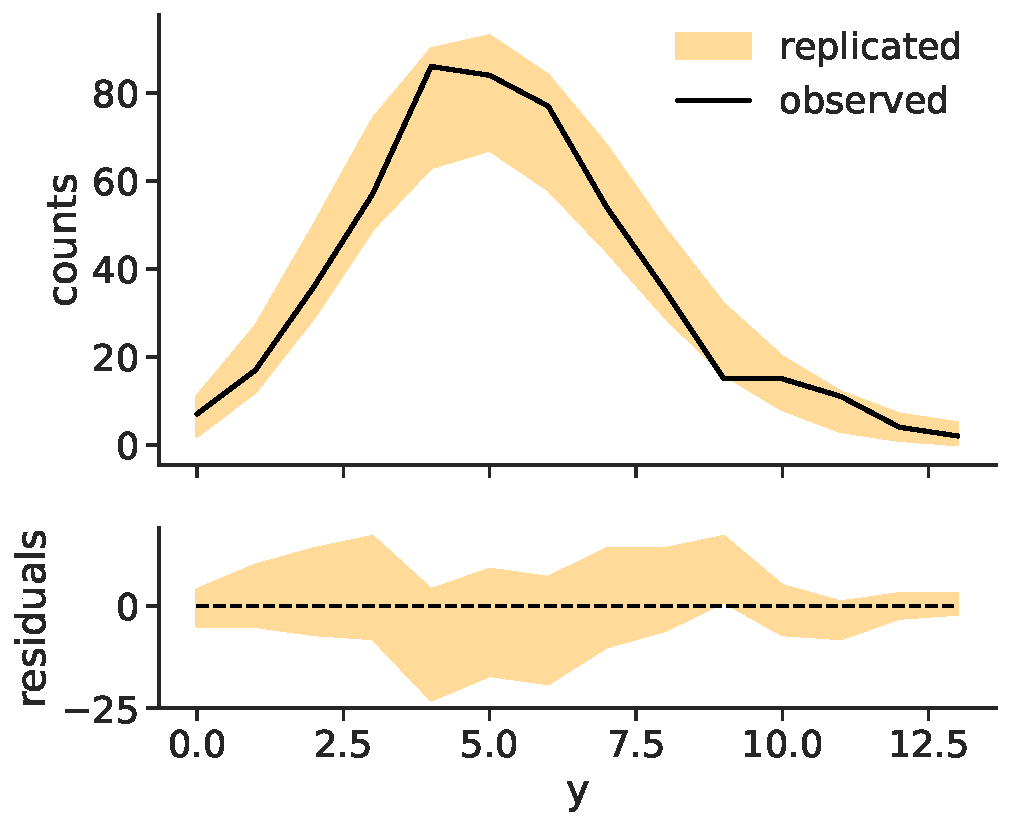
\includegraphics[width=\linewidth]{figures/ch2/poisson/predictive_check_1.pdf}
\caption{Posterior Predictive Check}
\end{subfigure}
\caption{Predictive Checks for the Poisson Model, showing the 95\% HDI of the replications of the original data $y$.
  Prior predictive check, generating sparse but reasonably distributed predictions around the data without
extreme values (a). Posterior predictive check, showing adaptation to the data (b).}
\label{fig:pois_pc}
\end{figure}
\begin{description}
\item[Posterior Predictive Checks] use samples from the posterior distribution and are employed to assess the model's
  fit to the observed data. Given an original dataset $y$ and model parameters $\theta$, sampling replicated data from the likelihood
  using parameters obtained from the posterior corresponds to sampling
  from what is known as the posterior predictive distribution:

\begin{equation}
p(y^{\text{rep}}\mid y)=\int p(y^{\text{rep}}\mid\theta)\cdot p(\theta\mid y),\mathrm{d}\theta.
\label{eq:postpred}
\end{equation}

\item[Prior Predictive Checks] generate replications from the priors, effectively sampling from the same distribution
  as posterior predictive checks in the limit of no observed data, which in this case is denoted as prior predictive
  distribution:

\begin{equation}
p(y^{\text{rep}})=\int p(y^{\text{rep}}\mid\theta)\cdot p(\theta)\mathrm{d}\theta.
\label{eq:priorpred}
\end{equation}

  They are valuable for diagnosing issues with the priors, such as whether they might be overly vague and generate
  extreme values or, conversely, be more informative but poorly positioned and shaped.
\end{description}

Figure \ref{fig:pois_pc} presents prior and posterior predictive checks for the Poisson
model, overlaying 100 replications on top of the observed data. The distribution of residuals is also plotted to facilitate visual inspection
While data visualization is a powerful tool that should be integrated into every workflow \cite{gabry2019visualization}, there is no standardized
approach for creating informative predictive check plots, especially for more complex models. Moreover, qualitative assessment
may be supplemented with quantitative scores for batch testing and automation. As previously mentioned, this can be
achieved by calculating summary statistics such as the mean, standard deviation, or quantiles for each replicated
dataset. If the model accurately replicates the data, the resulting distributions of these statistics should cover
the values derived from the observed data. Integrating the test statistics distributions from the observed value to
infinity provides a "p-value"-like score indicative of the goodness of fit, with optimal fit being represented by $p_{fit}\sim 0.5$. It is essential to note that this "p-value" score is not calibrated in the frequentist sense and does not follow a uniform distribution.

Predictive checks are implemented in Stan using the generated quantities block. Below is an example of how predictive
checks can be incorporated into the Poisson model discussed in the previous sections. The mean and standard deviation of each replicated dataset are also included in the output to be used as test statistics.

\begin{lstlisting}[language=Stan]
generated quantities {
array[N] int<lower = 0> y_rep = poisson_rng(rep_array(lambda, N));
real<lower = 0> mean_y_rep = mean(to_vector(y_rep));
real<lower = 0> sd_y_rep = sd(to_vector(y_rep));
}
\end{lstlisting}

By utilizing a flag data variable to switch between prior and posterior sampling, this same code can be employed for
both prior and posterior checks. Figure \ref{fig:pois_pc2} depicts the boxplots representing the distribution of the
means and standard deviations computed from each predicted dataset of Fig \ref{fig:pois_pc}, along with their corresponding p-values.
\begin{figure}[t]
  \begin{minipage}{0.6\linewidth}
    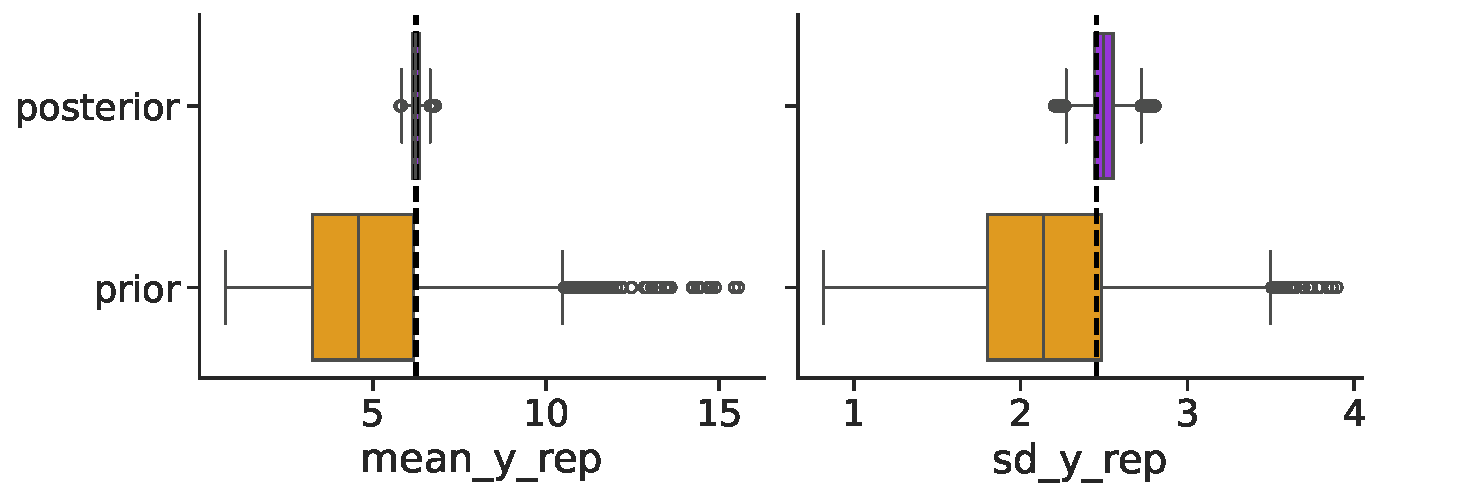
\includegraphics[width=\linewidth]{figures/ch2/poisson/cat_plot_1.pdf}
  \end{minipage}
  \hfill
  \begin{minipage}{0.4\linewidth}
    \begin{tabular}{lrr}
\toprule
 & mean\_y\_rep & sd\_y\_rep \\
\midrule
posterior & 0.50 & 0.69 \\
prior & 0.28 & 0.26 \\
\bottomrule
\end{tabular}
  \end{minipage}
    \caption{Boxplots for prior and posterior predictive checks of the Poisson model, representing the distributions for the mean and standard deviation of the replicated data, used as test statistics. The table shows their p-values.}
    \label{fig:pois_pc2}
\end{figure}

\subsection{Sensitivity analysis}
Sensitivity analysis, also referred to as robust analysis, focuses on evaluating the extent to which posterior
inferences are affected by variations in the prior, data, or model \cite{ruggeri2005robust}. 
Generally speaking, one of the most important characteristics of a model consists in the range of possible
configurations of its assumptions that determines similar results, with a more robust model producing consistent results for a wider range of variation. Due to the impossibility to choose a univocal prior distribution, prior sensititvity analysis is the major focus of these studies, which aim to determine wheter it is possible to obtain consistent results without needing incredibly specific assumptions.

The most straightforward way to gauge the influence of priors on the posterior consists in refitting the model under
different conditions and comparing the results, which is known as the informal approach. Considering the Poisson model
example, figure \ref{fig:poisson_sens} illustrates the sensitivity of the posterior distribution for the rate $\lambda$
to different choices of prior location and data count. In this case, the mean of the gamma prior $\mu=\frac{\alpha}
{\beta}$ is modified while keeping the variance fixed at $\sigma_{\text{prior}}^2=5$. The posterior medians and $95\%$ Highest Density
Interval (HDI) intervals are depicted as a function of $\mu$ and $N$. Notably, even when considering a prior centered on
$\mu=50$, which is more than 20 standard deviations away from the true value of $\lambda$, the results illustrate the
robustness of such a simple model and how the influence of priors diminishes with increasing amounts of data. These
results, obtained with Stan, are consistent from what is expected from the analytical solution of Sec \ref{sec:example}.

\begin{figure}[t]
\centering
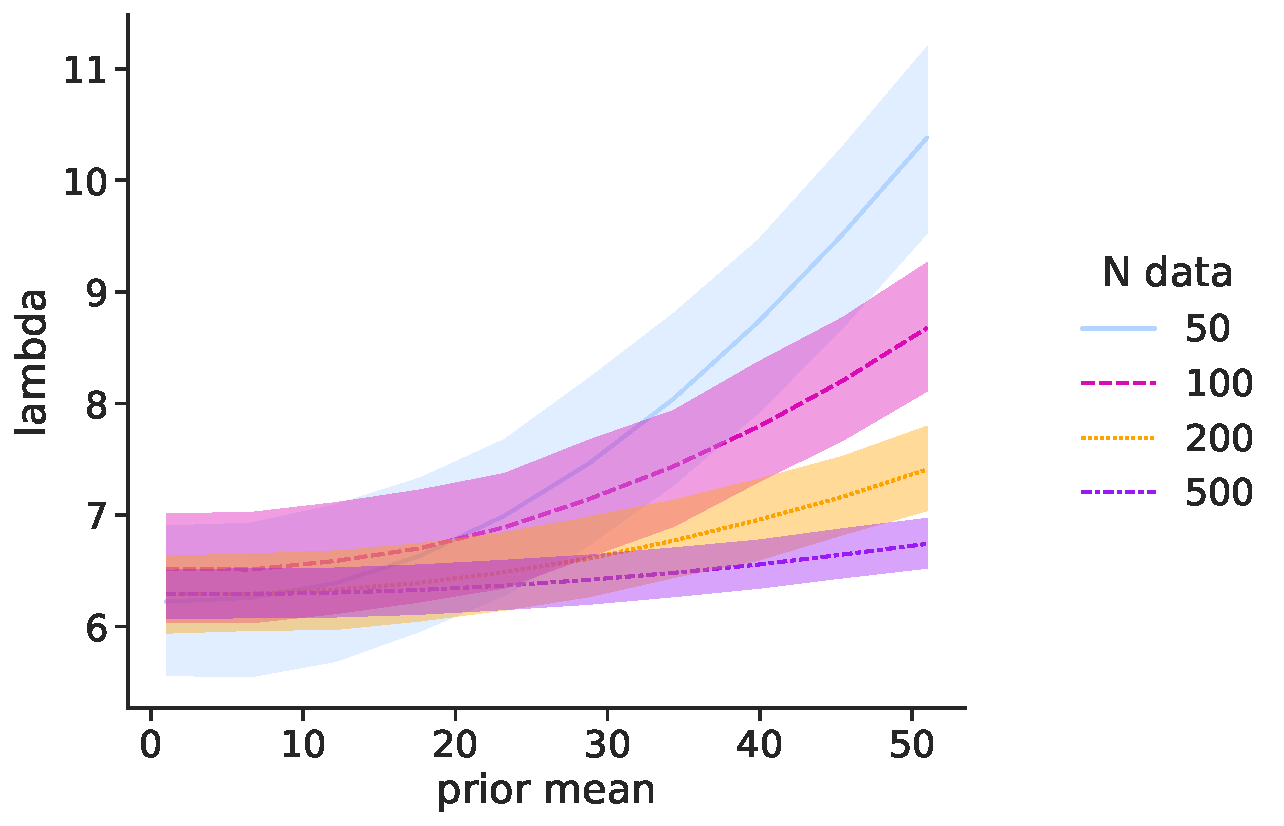
\includegraphics[width=0.85\linewidth]{figures/ch2/poisson/sens_0.pdf}
\caption{95\% HDI of posterior samples of $\lambda$ as a function of prior mean and number of data. Only the mean of
the Gamma prior is varied, while its variance is fixed to $\sigma_{\text{prior}}^2=5$. In this simple model, enough data results in stable estimates even for completely unreasonable priors.}
\label{fig:poisson_sens}
\end{figure}

Apart from the informal approach of varying the input and refitting the model, which can easily become prohibitively expensive for complex problems, there are two other main classes of prior sensitivity analysis, assessing global and local robustness respectively. 
Global robustness involves considering the entire set of priors that align with the chosen prior information using a formalized class, such as $\epsilon$-contaminated priors, where a base prior $p_0(\theta)$ is mixed with other possible choices with a probability $\epsilon$, propagating the uncertainty on priors to the posterior. The objective is to determine the range covered by the posterior mean as the prior distribution varies within this set. To achieve this, one typically identifies the extremal priors in the set, those that yield the maximum and minimum posterior means. While not requiring to fit the model for every prior in the class, this process can become intricate when dealing with multidimensional problems.

On the other hand, local robustness is interested in the rate of change in inferences, with respect to changes in the prior, and uses differential techniques to evaluate the rate. 
For example, consider a parametric class of priors $p(\theta\mid\alpha)$, which have a common functional form whose shape is determined by the quantity $\alpha$, which in this context is known as an hyperparameter. 
The local sensitivity of any expectation $f$ computed over the posterior is then given by its derivative with respect to $\alpha$ evaluated at a certain $\alpha_0$:
\begin{equation}
    \frac{\partial f(p(y\mid \theta,\alpha))}{\partial\alpha}\rvert_{\alpha=\alpha_0}
\end{equation}
Local sensitivity measures are generally more straightforward to compute in complex scenarios compared to global measures, but their interpretation and calibration may not always be as clear. 


\subsection{Hypothesis testing}
Hypothesis testing plays a central role in standard scientific practice, aiming to asses whether the observed data
provides support for a particular statement. However, it is also the subject of ongoing discussion both around its
philosophical foundations and practical implementation. While the use of p-values commonly employed in frequentist
statistics has faced significant criticism \cite{wasserstein2016asa}, at the same time Bayesian statistics offer no unified approach to hypothesis testing. 

One of the most common Bayesian hypothesis testing methods utilizes the Bayes factor (BF) \cite{kass1995bayes}. Given two competing models, denoted as $M_1$ and $M_2$, with parameters $\theta_1$ and $\theta_2$ and data $y$, the Bayes factor is defined as:

\begin{equation}
BF = \frac{p(y\mid M_2)}{p(y\mid M_1)} = \frac{\int p(y\mid \theta_1, M_1)p(\theta_1\mid M_1)d\theta_1}{\int p(y\mid \theta_2, M_2)p(\theta_2\mid M_2)d\theta_2}
\end{equation}
In this equation, the dependence on each model has been explicited in the likelihoods and priors. Each term $p(y\mid M_{i})$ in the ratio is known as the evidence, and corresponds to the normalization constant of Bayes' theorem that is usually neglected when computing the posterior with MCMC algorithms.
The Bayes factor resembles a likelihood ratio, but it averages the likelihoods over the entire parameter space rather
than using maximum values. Additionally, the BF naturally penalizes overfitting, as including more parameters expands the space over which the likelihood is averaged.

The ratio can be interpreted as providing the evidence in favor of one model over another through the probability of
observing the data, given each model. A value of $BF>1$ indicates increasing preference for $M_2$. While various scales for interpretation are cited, Bayes factors between 5 and 10 are generally considered to provide substantial evidence for $M_2$, and $BF>10$ indicates strong evidence.

However, the Bayes factor faces some critical issues. The first problem is its strong dependence on the priors of each
model $p(\theta_i\mid M_i)$. Contrary to the posterior, which usually overcomes the priors with sufficiently informative
data, the Bayes factor always remains sensitive to the details of the specified prior distributions. 
Consequently, extensive sensitivity analysis is necessary when using this method. A possible robust approach involves obtaining the lower bound of the Bayes factor for entire classes of priors instead of using a single prior distribution.

The second problem is the computational cost of integrating the likelihood over the entire parameter space to obtain the
evidence. While in some specific instances the BF can be expressed in a simpler form that allows for easier computation
\cite{heck2019caveat},
in most cases it is necessary to estimate $p(y)$ directly. Doing so accurately requires many
more ($>50\times$) MCMC samples than those used for posterior sampling, and the resulting estimates still cannot be used directly, but
must also be refined with reweighting methods like bridge sampling \cite{bridge}.

Due to these limitations, many researchers choose alternative hypothesis testing methods over the Bayes factor. One
common and simpler approach involves parameter estimation and posterior intervals. As an example, considered a specific
case of a point
null hypothesis $H_0$, corresponding to a model with one parameter fixed to certain value $\theta = 0$, while the
alternative hypothesis $H_1$ leaves $\theta$ as a free parameter. In the interval-based approach to hypotheses testing,
$H_0$ is rejected with a certain credibility $\alpha$ if the respective credible interval of the posterior distribution
for $\theta$ given $H_1$ does not contain $\theta = 0$.


The adoption of this method has sparked considerable debate, as it can yield different results than the Bayes factor for
the same data \cite{wagenmakers2020principle}. However, it can be shown that these apparent inconsistencies arise because
interval estimation implicitly assigns a prior probability of 1 to $H_1$, excluding all other hypotheses  \cite{campbell2023twofaces}. This differs from the priors used for the Bayes factor, which require both $Pr(H_1)$ and $Pr(H_0)$ to be nonzero, leading to different conclusions in many scenarios.

To reconcile these approaches, one can construct a model that encompasses both hypotheses with appropriate priors. This can be achieved using Bayesian Model Averaging, which combines samples after fitting, or by building a model with a discrete parameter that switches between the two hypotheses with a certain probability. The posterior of this discrete parameter allows to recover the Bayes factor.


\subsection{Comparing the predictive performance}
Hypotheses testing compares two models based on the evidence provided only by the observed data.
However, another possible goal of data analysis is to construct a model that is not only supported by the
available data, but also able to generate meaningful predictions. While these two approaches are closely related, the
second is especially useful in cases where specific hypotheses
cannot be established, and it is instead necessary to engage in model building and selection techniques to improve the understanding of the data generating process.
Even when all considered models exhibit mismatches with the data, it remains
valuable to evaluate their accuracy and determine potential avenues for improvement. 

The task of confronting the performance of different
models extends beyond identifying the best fit to the data, as this approach inevitably leads to overfitting. A
more robust heuristic involves assessing how a model is likely to perform on new, unobserved data, thereby automatically
penalizing overfitting. Because of this, the following comparison techniques will focus on providing a measure of the
predictive accuracy of a model.

An estimate of the disparity between models can be constructed considering the information entropy, which quantifies the
uncertainty intrinsic in a distribution \cite{mcelreath2020statistical}. For $N$ observations with respective probabilities  $p_i$, it is defined as:

\begin{equation}
    H(p)=-\sum_i^N p_i \log p_i
\end{equation}
The distance between the true data generating process defined by $p^{\text{true}}$ and the model  $p$ is then given by
the Kullback-Leibler divergence, which is closely related to the information entropy:
\begin{equation}
    D_{KL}(p^{\text{true}}, p) = \sum_i^N p_i^{\text{true}}\log p^{\text{true}}_i - p^{\text{true}}_i\log p_i
\end{equation}


This divergence can be interpreted as the additional uncertainty introduced by using $p$ to approximate
the distribution $p^{\text{true}}$. 


The central quantity involved in predictive model comparison, denoted as the "expected log pointwise predictive density" (elpd), is
constructed from the second term of the KL divergence.
The definition of the elpd considers $N$ observed data $y$ independently modeled with parameters $\theta$ and
likelihood $p(y|\theta) = \prod_{i=1}^{N} p(y_i|\theta)$, and constructs the second term of the KL divergence relative
to the distribution of unobserved data $\tilde{y}$:

\begin{equation}
\text{elpd} = \sum_{i=1}^{N}\int p^{\text{true}}(\tilde{y_i}) \log p(\tilde{y_i}|y) d\tilde{y_i}
\end{equation}
where $p(\tilde{y}|y)$ is the posterior predictive distribution of Eq \ref{eq:postpred}. Since $p^{\text{true}}$ is
usually inaccessible, it is only possible to construct a biased estimator the elpd. However, the core feature of model
comparison is that when computing the elpd for two different models the bias induced by not knowing $p^\text{true}$
is the same for both estimates, allowing for a thruthful relative comparison. 
\subsubsection*{Information criteria}
The various methods employed in model comparison mainly differ in the way the elpd estimate is constructed.
Many of the proposed approaches, historically known as information
criteria, start from the log pointwise predictive density (lpd) or a similar quantity:
\begin{equation}
\text{lpd}=\sum_{i=1}^{N} \log p(y_i|y) = \sum_{i=1}^{N} \log\int p(y_i\mid\theta) p(\theta|y) d\theta
\end{equation}
The lpd can be easily computed after obtaining $S$ draws from the posterior  $\theta_{1\ldots S}$ :
\begin{equation}
    \widehat{\text{lpd}}=\sum_{i=1}^{N}\log\left(\frac{1}{S}\sum_{s=1}^{S}p(y_{i}\mid \theta_{s})\right).
\end{equation}
However, since the lpd only considers observed data, it systematically overestimates the elpd and doesn't penalize
overfitting. To address this, a penalty term representing the effective number of parameters
$n_{eff}$ can be introduced. 
Between the many available information criteria one of the most used is the Widely Applicable Information
Criterium (WAIC) \cite{watanabe2013widely}, which is defined as:
\begin{eqnarray}
  \widehat{n}_{\mathrm{waic}} &=&\sum_{i=1}^{N}\mathrm{var_{post}}\left(\mathrm{log}\,p(y_{i}|\theta)\right),\\
   % \widehat{n}_{\mathrm{waic}} &=&\sum_{i=1}^{N}\frac{1}{S-1}\sum_{s=1}^S\left(\log p(y_i|\theta^{s})- \overline{\log p(y_i|\theta)}\right)^2\\
    \widehat{\text{elpd}}_{\mathrm{waic}} &=& \widehat{\text{lpd}}- \widehat{n}_{\mathrm{waic}}
\end{eqnarray}
As an example, consider a linear regression model with data $x$ and $y$. Vague priors are
assigned to the intercept $\alpha$, slope $\beta$ and dispersion $\sigma$: 
 \begin{eqnarray}
   \alpha &\sim&  \text{normal}(0, 10) \\
   \beta &\sim &\text{normal}(0, 10) \\
   \sigma& \sim& \text{exponential}(10)\\
   y &\sim &\text{normal}(\alpha + \beta x, \sigma)
\end{eqnarray}


Let's compare this model to a simpler version without the intercept, considering $N=20$ data simulated from
$\alpha=0.2$, $\beta=0.5$, $\sigma=0.5$. To compare Stan models using WAIC, it is necessary to add the unnormalized
likelihood for each datapoint to the output using the generated quantities block:
\begin{lstlisting}[language=Stan]
generated quantities {
  vector[N] log_lik;
  for (n in 1:N) {
    log_lik[n] = normal_lpdf(y[n] | x[n] * beta + alpha, sigma);
  }
}
\end{lstlisting}
Once the models have been fitted, the WAIC estimate of the elpd can be obtained using ArviZ, with higher elpd indicating
better predictive performance. Since an estimate can be computed for every data $y_i$, the variance between single data
estimates represents an appromixate standard error on the total computed elpd:
\begin{equation}
  \sigma_{\text{elpd}} = \sqrt{N \text{var}(\text{elpd}_i)} 
\end{equation}
When interpreting the elpd, it is then necessary not only to consider which of the models provides the highest 
value, but also if
the difference in elpd between them is significant with respect to the standard errors on the estimates. The posterior predictive checks and results for the comparison of the two linear models are shown in Fig.\ref{waic}, with WAIC favoring the inclusion of the intercept.
\begin{figure}[t]
  \begin{minipage}{0.5\linewidth}
    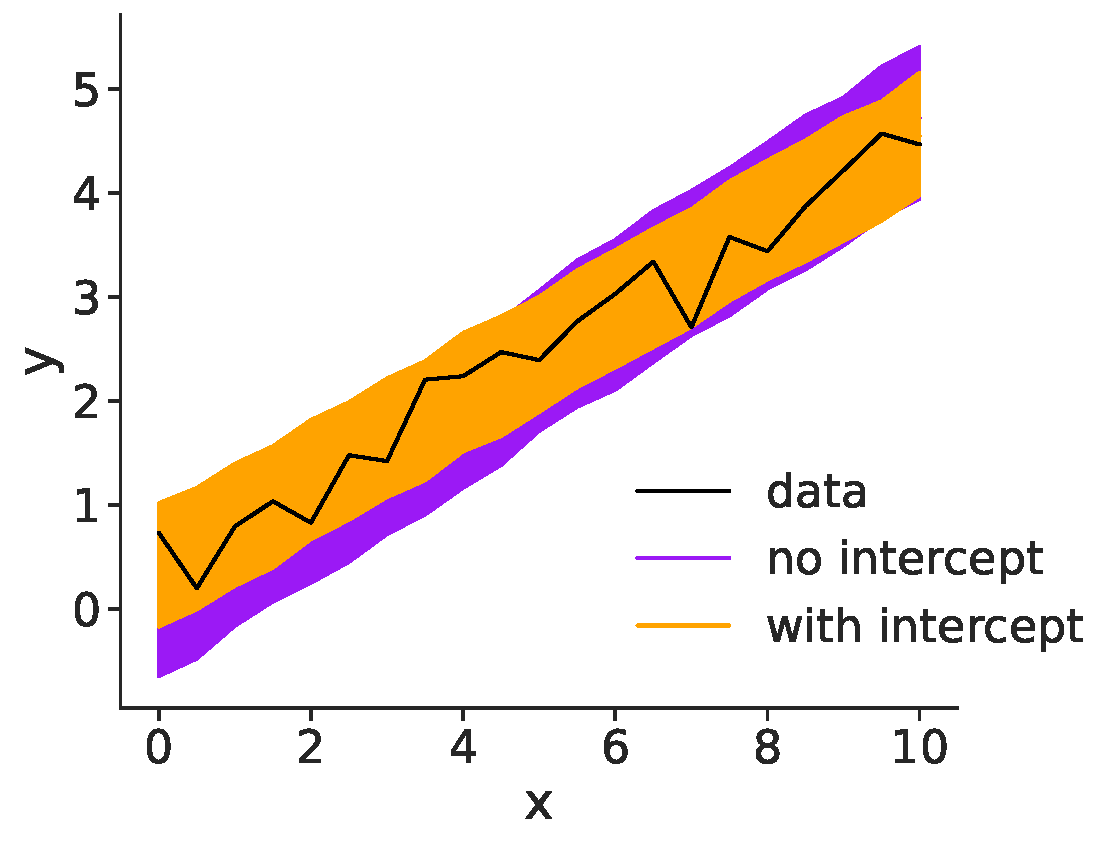
\includegraphics[width=\linewidth]{figures/ch2/linear/ppc_compare_0.pdf}
  \end{minipage} 
  \begin{minipage}{0.4\linewidth}
   \begin{tabular}{lrrr}
\toprule
 &  $elpd_{waic}$ & $\sigma_{\text{elpd}}$ & $n_{eff}$ \\
\midrule
no intercept   &      -4.6 & 2.6 &    1.4 \\
with intercept &       3.4 & 1.7 &    2.2 \\
\bottomrule
\end{tabular}
  \end{minipage}
\caption{Posterior predictive checks for linear regression models with or without intercept parameter, showing the 95\%
  highest density intervals of the replicated datasets below the observed data. The table contains the estimated elpd of each model using WAIC, its standard error and the effective number of
parameters.}
\label{waic}
\end{figure}

\subsubsection{Cross validation}
Another common strategy to asses predictive accuracy is to use only part of the data to fit the model and use the rest
to test it. To avoid discarding useful data, the sample is divided in a number of chunks, called “folds.” The
model is asked to predict each fold after training on all the others. An estimate of predictive accuracy is then
provided by averaging the scores for each fold.
Usually, only one observation at a time is excluded, implementing what is known as leave-one-out cross validation (LOOCV)
 \cite{vehtari2017practical}. With
$N$ observations and $S$ samples from the posterior, LOOCV estimates the elpd as:
\begin{equation}
    \mathrm{elpd}_{\mathrm{loo}}=\sum_{i=1}^{N}\log p(y_{i}|y_{-i})=\sum_{i=1}^N \log \frac{1}{S}\sum_{s=1}^S p(y_i\mid \theta{s,-i})
\end{equation}
Where $\theta_{s,-i}$ are samples from the posterior computed using the dataset without the i-th observation.
The key prolem with this method is that it requires to compute as many posteriors as datapoints.
Fortunately, LOOCV can be efficiently estimated using only one fit of the model over the full data. This approximation is
called Pareto smoothed importance sampling cross-validation (PSIS). Each observation $y_i$ defines a set of
weights for the full posterior samples:
\begin{equation}
  r_i(\theta_{s})={\frac{1}{P(y_{i}|\theta_{s})}}
\end{equation}
These weights are a measure of how much each observation influences the posterior. When the weights for the i-th
observation are applied to the posterior samples, the result is a set of samples resembling those from the posterior
computed without that datapoint. Reweighting the full posterior for each observation and combining the results allows
approximating the LOOCV score as:
\begin{equation}
  \mathrm{elpd}_{\mathrm{IS}}=\sum_{i=1}^{N}\mathrm{log}\,\frac{\sum_{s=1}^{S}r_i(\theta_{s})p(y_{i}|\theta_{s})}
  {\sum_{s=1}^{S}r_i(\theta_{s})}
\end{equation}

\begin{figure}[t]
  \begin{minipage}{0.4\linewidth}
   \begin{tabular}{lrrr}
\toprule
 &  $\text{elpd}_{\text{loo}}$ & $\sigma_{\text{elpd}}$ &  $n_{eff}$ \\
\midrule
no intercept   &     -4.7 & 2.6 &   1.4 \\
with intercept &      3.3 & 1.8 &   2.2 \\
\bottomrule
\end{tabular}
  \end{minipage}
  \hfill
  \begin{minipage}{0.5\linewidth}
    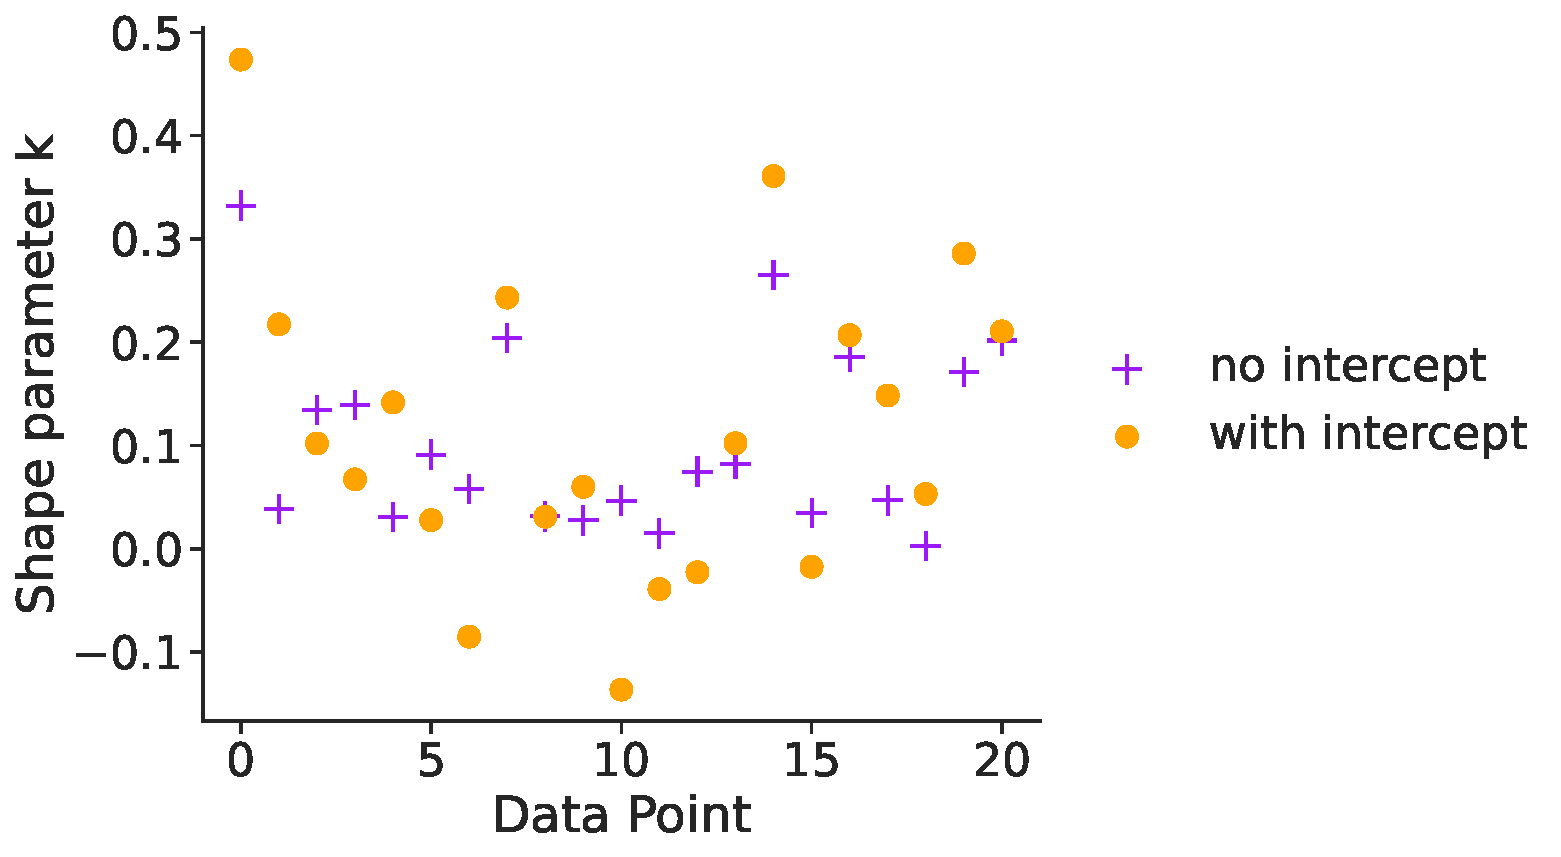
\includegraphics[width=\linewidth]{figures/ch2/linear/loo_khat_0.pdf}
  \end{minipage} 
\caption{Estimated Pareto distribution's $\hat{k}$ for each data point computed using PSIS-LOO for the linear models. All values are less than
  0.5, indicating no particularly influential data and robust approximation of the elpd. The table contains the
estimated elpd, its standard error and the effective number of parameters, with values almost equal to those obtained
with WAIC.}
\label{loo}
\end{figure}
However, this estimate is very sensitive to possible large weights due to particularly informative data, which may
introduce bias and very large fluctuations. 

The importance sampling approximation can be made more robust considering that the weights roughly follow a Pareto distribution:
\begin{equation}
  \text{Pareto}(r\mid\mu,\sigma,k)=\sigma^{-1}\left(1\ +k(r-\ \mu)\sigma^{-1}\right)^{-\frac{1}{k}-1}
\end{equation}
For each left-out observation, this distribution is fitted to the largest weights and then used to smooth extreme
values, obtaining $N$ estimates of its parameters. The shape parameter $k$ is of special interest since it provides a way to asses the reliability of the approximation. If for a certain observation $y_i$ the fit results in  $k>0.5$, the Pareto distribution has infinite variance, indicating a highly influential datapoint that may induce biased estimates.
Due to the ability of PSIS to provide feedback about its reliability and the smaller bias of LOOCV in computing the elpd with respect to WAIC,
LOOCV has become one of the primary methods for bayesian model comparison. Moreover, it can be shown that WAIC asymptotically
approaches LOO in the limit of infinite data. Beacuse of this, WAIC is still employed as a computationally easier
alternative to cross validation.

Using LOOCV with Stan also requires computing the likelihood in the generated quantities block, exactly as WAIC. The
test can also be performed using ArviZ, which provides various methods to check the approximation, for examples by
plotting the obtained shape parameters as in Fig \ref{loo}.


\section{Multilevel models}


\subsection{Measurement error}
Instead of being assigned a fixed prior, some parameters in a model can themselves be governed by a distribution dependent on other parameters. This distribution is known as a hierachical prior, and its parameters are denoted as hyperparameters. The latter also have a prior distribution, often refferred to as the hyperprior. This creates a
multilevel structure where the basic parameters can share information between each other trough the hierarchical prior,
resulting in many powerful applications that often have no frequentist counterpart, but requires some extra
considerations regarding model implementation. This final section of the chapter presents two multilevel models that could be useful
in physics applications.


The first example shows how it is possible to extend many models in order to consider data measured with a certain
error. For instance, consider $N$ data \(x_{\text{meas}}\) and $y_{meas}$, measured with known dispersions \(\sigma_x\) and
$\sigma_y$. A common task would require to fit a function $f(x)=y$ considering the error on both. In usual applications
a variant of the ordinary least squares fit is used, which however provides biased results when both the errors are significant and $f$ is nonlinear. 
Instead, the bayesian model does not approximate the relation between $x_{\text{meas}}$ and $y_{\text{meas}}$. To do so,
it introduces \(N\) parameters \(x_{\text{true}}\), representing the true values from which \(x_{\text{meas}}\) has originated. These parameters can then be given a hierarchical prior, which 
describes how the error has originated. 
The central aspect of this approach is that the hierarchical prior can describe many kinds of measurement error, not just gaussian, for example allowing to consider rounding errors or approximations in the analysis.
The true values \(x_{\text{true}}\) and eventual additional parameters in the hierarchical prior are then regularized by the respective hyperpriors. The errors on $y$ can also be modeled in different ways.

As an example, consider data measured with normal error. In this case, each \(x_{\text{meas}}[i]\) is considered to
originate from a normal distribution with mean \(x_{\text{true}}[i]\) and standard deviation $\sigma_x$. The same is
assumed for \(y_{\text{meas}}\), which will be distributed according to a normal with mean $y_{\text{true}}
=f(x_{\text{true}})$ and dispersion $\sigma_y$. In this case, the hyperprior for all \(x_{\text{true}}\) is another normal distribution used to constrain the parameters to their expected range by choosing its mean $\mu$ and deviation $\tau$. The model is specified as:
\begin{eqnarray}
x_{\text{true}} &\sim& \text{normal}(\mu, \tau)\\
x_{\text{meas}} &\sim& \text{normal}(x_{\text{true}}, \sigma_x)\\
y_{\text{meas}} &\sim &\text{normal}(f(x_{\text{true}}), \sigma_y)
\end{eqnarray}
As described in Sec \ref{sec:repar}, it is important not only to define the general form of a model, but also to
implement a specific parametrization that avoids problematic geometries in the distribution explored by the MCMC
algorithm. 
The non-centered parameterization of this measurement error model uses \(N\) standard normal parameters \(z\) instead of \(x_{\text{true}}\), improving the efficiency of the sampler:
\begin{eqnarray}
z &\sim& \text{normal}(0, 1) \\
x_{\text{true}} &= &\tau z + \mu
\end{eqnarray}

While using a new parameter for each data point may seem concerning, Stan is able to easily handle problems of this kind even with thousands of parameters. 
It is also possible to leave $\sigma_y$ as an additional parameter, however this can be done only if the error bands for \(x\) do not overlap, since this results in multiple possible valid configurations for \(x_{\text{true}}\). Finally, $\mu$ and $\tau$ can also be used as free parameters, automatically selecting the scale and position of the hyperprior.


% The second is the possibility of executing unbinned fits of convolved distributions, even when the analytic form of the convolution is not available. This may be done when \(x_{\text{meas}}\) can be sampled from a distribution that is determined by a location parameter that can be assigned to \(x_{\text{true}}\), such as the normal. In this way, \(x_{\text{meas}}\) is modeled as a sum of two random variables, with its density being the convolution between the underlying distribution of \(x_{\text{true}}\) and that of the error.


\subsection{Gaussian processes}
Gaussian processes (GP) are a bayesian machine learning technique that can be used to interpolate the available data
and generate predictions for new input values, even when no functional form is available \cite{mackay1998introduction}.
Being a bayesian method, one of their most useful properties is that they automatically quantify the uncertainty on their predictions.

The core intuition behind GPs consists in representing an arbitrary function as a series of random variables, one for
each point of the function. All of these random variables are collected in a multivariate distribution, with each variable
corresponding to an additional dimension, resulting in an infinite-dimensional distribution for continuous functions. The training data fix some points of the function, and predictions are
obtained from the correlations between these fixed points and the other variables in the many-dimensional distribution.

%This distribution can be thought of as a possibly infinite collection of random variables, each corresponding to a potential input. 

Modeling a set of output values \(f\) given their respective inputs \(x\), a Gaussian process defines this distribution as a multivariate normal with as many dimensions as there are inputs:
\[
f \sim \text{multivariate normal}(\mu(x),\Sigma(x)) \label{eq:gaussian-process} \tag{2.58}
\]
Instead of having a fixed mean and standard deviation, this multivariate normal is characterized by two fundamental components: the mean function \(\mu(x)\) and the covariance function \(\Sigma(x)\). Counterintuitively, the mean function does not significantly impact inference and can often be set to zero without loss of generality, but it will affect predictions far from any data, which will tend to be distributed around the mean. The covariance function, on the other hand, plays a crucial role, defining the distribution over functions by quantifying the correlations between different outputs as a function of the input points. It must yield a positive definite matrix for any input configuration and is often referred to as the kernel of the Gaussian process. A widely used choice is the exponentiated quadratic kernel, which produces a smooth interpolation of the data. It is given by:
\[
\Sigma(x | \alpha, \rho)_{i,j} = \alpha^2 \exp\left(-\frac{(x_i - x_j)^2}{2\rho^2}\right) \label{eq:exponential-quadratic-kernel} \tag{2.59}
\]
In this expression, \(\alpha\) and \(\rho\) represent the hyperparameters of the Gaussian process model. Intuitively,
\(\alpha\) controls the strength of the correlation between output points, resulting in smoother interpolations when
increased. On the other hand, the parameter \(\rho\) can be interpreted as the length-scale, determining the range of
the smoothing effect. Common models employing Gaussian processes combine the underlying function \(f\) with a
distribution describing how the outcomes are dispersed around \(f\). A full model specification with $N$ outcomes $y$
dispersed normally around  $f$ with standard deviation \(\sigma\), including priors for all parameters, is given by:

\begin{eqnarray} \label{eq:GP}
\rho &\sim & \text{gamma}(5,1)\\
\alpha &\sim & \text{normal}(0,1) \\
\sigma &\sim & \text{normal}(0,1) \\
f &\sim & \text{multivariate normal}(0,\Sigma(x | \alpha,\rho)) \\
y &\sim & \text{normal}(f,\sigma) \label{eq:GPfin}
\end{eqnarray}
This formulation, known as the latent variable GP, requires \(N\) parameters \(f\) to model the distribution of functions. If the outcome \(y\) is normal, as in this case, these parameters can be integrated out of the likelihood, combining the last two statements into:
\[
y \sim \text{multivariate normal}(0,\Sigma(x | \alpha,\rho) + \mathbb I_N\sigma^2) \label{eq:reduced-likelihood} \tag{2.65}
\]
This greatly reduces the computational requirements. Posterior predictive checks and the mean posterior kernel for this
model are shown in Fig \ref{fig:GP}.
\begin{figure}[t]
    \begin{subfigure}[b]{0.5\linewidth}
    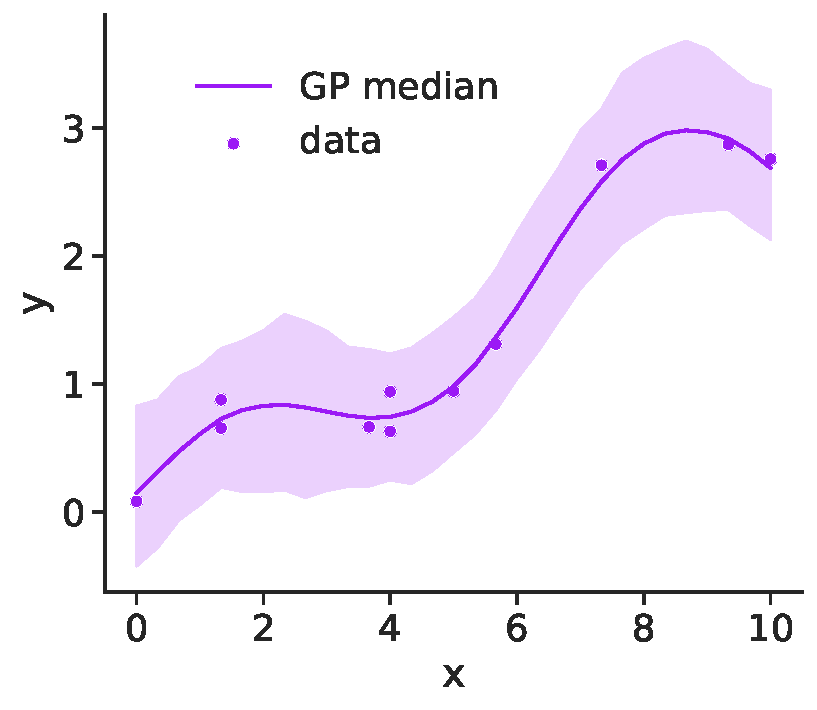
\includegraphics[width=\linewidth]{figures/ch2/GP/GP_0.pdf}
\caption{}
\end{subfigure}
\hfill
\begin{subfigure}[b]{0.5\linewidth}
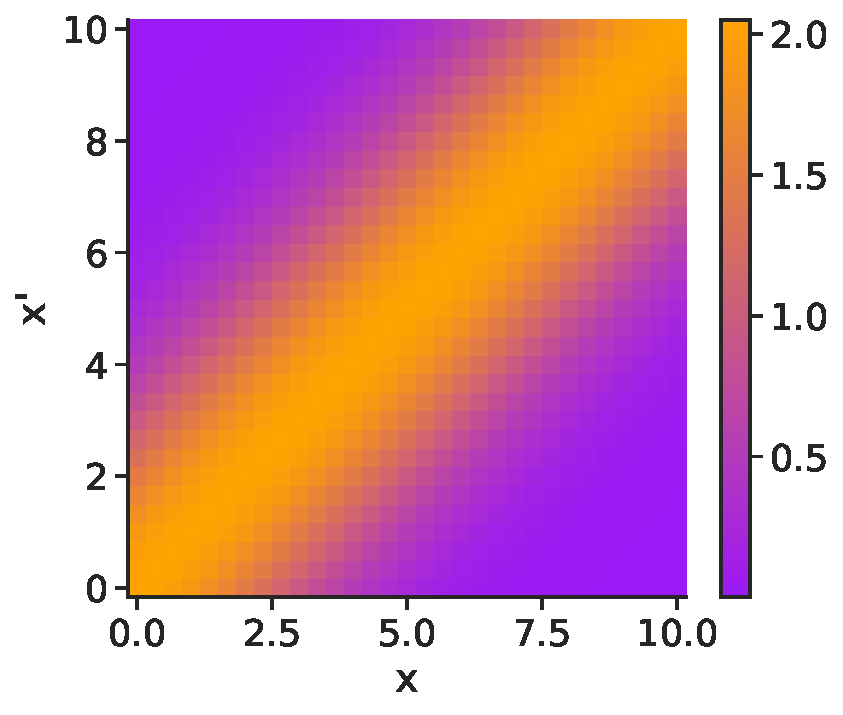
\includegraphics[width=\linewidth]{figures/ch2/GP/kernel_0.pdf}
\caption{}
\end{subfigure}
\caption{Posterior predictive check of Gaussian process regression for normal outcomes with dispersions $\sigma=0.2$, showing the median and 95\%
HDI of the predictions (a). Exponentiated quadratic kernel computed from the posterior means of the hyperparameters \(\alpha\) and \(\rho\)
(b).} 
\label{fig:GP}
\end{figure}

It is also possible to model the outcomes with another distribution dependent on the Gaussian process, for example, a
Poissonian or a Bernoulli. In this case, the latent variable formulation must be used explicitly, thus requiring a
parameter for every data point and the hierarchical structure of Eq \ref{eq:GP}-\ref{eq:GPfin}.

Implementation of Gaussian processes is commonly written in Stan using the Cholesky
factored reparameterization, which is more efficient for large datasets (\(N > 100\)). The Cholesky decomposition of
\(\Sigma(x \mid \theta)\) is the lower triangular matrix \(L\) such that \(LL^T = \Sigma\). The GP parameters \(f\)
are obtained by multiplying a vector of normally distributed parameters \(\eta\) by \(L\) and adding the mean function
$\mu$:
\begin{eqnarray}
\eta &\sim &\text{normal}(0,1)  \\
f&=&\mu + L\eta
\end{eqnarray}
Once a Gaussian process has been trained on a dataset, it becomes a powerful tool for making predictions for new input
values. The inherent uncertainty captured by the multivariate distribution provides valuable insights into the reliability of these predictions, making Gaussian processes a versatile and widely used tool both in statistics and machine learning.


\newpage
\thispagestyle{empty}
\chapter{Data Analysis}
This chapter presents two applications of Bayesian data analysis to different parts of the calorimetric $^{163}$Ho spectrum measured
by Holmes. A preliminary section provides a brief description the data processing techniques used to obtain a
calibrated energy spectrum from the raw signals, and of the expected background. The first part of the
analysis focuses on the M1 peak, using experimental data from 16 detectors. A basic
model is established and then expanded in order to describe an eventual asymmetry of the peak and fit all the available
data simultaneously, providing a preliminary measurement of the M1 position and width. The second part estimates a
plausible upper limit on the neutrino mass that could be achieved by Holmes in the near future, focusing on prior
sensitivity analysis and providing robust estimates from simulations of a low-activity measurement campaing. The chapter
concludes with a simulation of data from 64 different detectors, showing that for the low available statistics and under
the assumption that the systematics of the detectors are distributed normally a simple fitting procedure can be
applied to obtain consistent results.
\section{Preliminary considerations}
\subsection{Data elaboration}
As outlined in Section \ref{sec:muMUX}, the signals from the Transition Edge Sensors are observed as phase changes in the circuit's response to a certain microwave frequency. The raw signals are acquired through a time derivative trigger, resulting in a collection of pulses with the same length. To obtain a well-calibrated energy spectrum, the raw data must be carefully processed and corrected for the non-ideal behavior of the detectors. This data elaboration phase involves several distinct steps, which are briefly presented here.

\subsubsection*{Preanalysis}
The basic informations extracted from each raw signal include its baseline, given by the pre-trigger samples, the raw
amplitude, the rise time $RT$, and the decay time $RD$. In the initial stage of data elaboration, these quantities are
used to categorize the signals into six distinct types based on their pulse shapes. These categories, determined through
a series of filtering operations with adjustable threshold parameters, are crucial for the rest of the processing:

\begin{description}
\item[Empty:] Events containing noise.
\item[Strange:] Events exhibiting shapes differing from what is expected. 
\item[Bad:] Signals rising on the tail of a previous pulse, for which accurate energy identification is challenging due to the TES non-linearity.
\item[Multiple event:] Pile-up pulses rising from the tail of a triggered signal.
\item[Coincidence:] Muons or natural radioactivity background interacting with multiple detectors at the same time.
\item[Good:] All events not falling into the previous categories.
\end{description}

\subsubsection*{Optimum Filter}
The optimum filter is employed to refine the raw signal amplitude into another estimator more suitable for energy
calibration. This method allows the construction and application of a frequency filter to the signal, theoretically
maximizing the signal-to-noise ratio under specific assumptions. Each sample $s_i$ of a pulse is considered to be a
linear combination of a constant factor $K$ related to energy, a noise component $n_i$, and an underlying medium pulse $m_i$, as in $s_i = K m_i + n_i$. Given an ergodic noise with power spectral density $N$ and a signal sampled at a sufficiently high rate, the optimum filter $H$ is constructed from the Discrete Fourier Transform (DFT) of the samples $S$ and of the mean pulse $M$:
\begin{eqnarray}
 H_i \propto \frac{M_i^*}{N_i}\\
s^{OF}_i = \text{DFT}^{-1}(H \cdot S)_i
\end{eqnarray}
In this case, $N$ is computed from the average DFT of the signals tagged as "empty," which contain noise, while the mean pulse is obtained from a series of "good" events corrected for their arrival time. The resulting filtered "good" signals and their amplitudes are used as the basis for the following elaborations.

\subsubsection*{Gain Drift Correction}
Detector gain and baseline fluctuate over time due to temperature and voltage variations, leading to different signal
amplitudes for the same energy deposition. This gain drift also leads to a correlation between signal amplitude and
baseline, which can often be approximated as linear or quadratic due to the fluctuations being small. This allows
correcting the gain drift by removing the correlation between these two quantities. Events within a mono-energetic peak are fitted with a low-order polynomial in the amplitude/baseline plane, and all data are corrected following the fit results.

However, this process is complicated by the sudden signal jumps that can be attributed to fluctuations in the number of
Phase Slip Lines, as detailed in Section \ref{sec:TES}. As shown in Fig. \ref{fig:drift}, events in these time
intervals feature a different slope between amplitude and baseline, and must be removed from the dataset since they
cannot be corrected properly. 

At this stage, the data is represented as an n-tuple associating each signal with a series
of parameters, such as its time of recording, raw amplitude, OF amplitude, rise-time, and decay-time. This allows
filtering events by selecting intervals of these parameters. The selected regions can be intersected or added, globally
constituting what is known as a cut. For the scope of drift correction, it is then necessary to perform a series of cuts
on the timestamps to select only events with the same correlation between amplitude and baseline. An algorithm utilizing
reinforcement learning is under development to automate this selection procedure.

To correct the gain drift simultaneously across the entire acquired energy range, the latter is divided into small regions where the coefficients of the correcting polynomial can be considered constant. The actual fit and removal of the correlation are carried out in the intervals containing the peaks from calibration sources or from $^{163}$Ho. The results are then extrapolated to the other regions of the spectrum using a spline.

\begin{figure}[t]
  \centering
  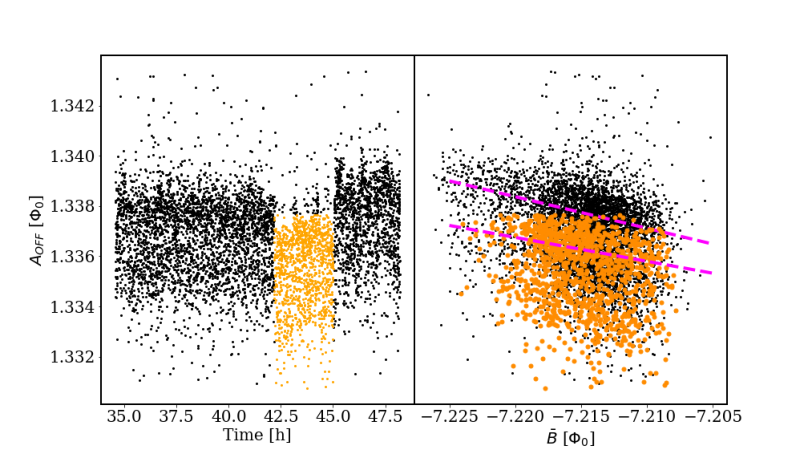
\includegraphics[width=0.77\textwidth]{figures/ch3/drift.pdf}
  \caption{Effect of sudden jumps in the detector response on the gain drift correction. Events in the corresponding
  time interval feature a different correlation between amplitude and baseline. Image taken from
\cite{borghesi2022toward}.}
  \label{fig:drift}
\end{figure}

\subsubsection*{Energy Calibration}
Leveraging the X-ray sources described in Section \ref{sec:holder}, the energy response of each detector is
calibrated using the processed signals obtained after applying the optimum filter and correcting the gain drift.
Calibration is performed by fitting some known X-ray peaks originating from the calibration source with one or more Gaussians. The peak energies $E_{OF}$ obtained
from the fit can be compared with the true known energies of the decays $E_{true}$. The calibration curve $E_{OF}
(E_{true})$ is then given by a low-order polynomial or a spline interpolating the points computed by fitting each peak. For the calibration of the data used in this thesis, a spline was employed.

The accuracy of the procedures leading to a calibrated spectrum can be verified by comparing the estimate of the energy
resolution $\Delta E$ obtained from the fit of a known X-ray peak, typically the $K_\alpha$ line of $^{55}$Mn, with that
given by the Noise Equivalent Power (NEP). The NEP determines $\Delta E$ from the noise power spectrum and the
detector's responsivity, assuming a delta signal for energy deposition, and can be considered as a lower bound for the
energy resolution reachable after calibration.

Achieving precise calibration is vital for characterizing the $^{163}$Ho spectrum, particularly in exploratory runs
aiming to characterize the decay spectrum by determining the parameters of the main Lorentzian peaks and measure the
$Q$-value. The calibration systematics will play a central role in the construction of the fit models used in this chapter.

\subsection{Expected Background and Background Rejection}\label{sec:expected}
For the Holmes experiment, background can be considered to originate from either pile-up events or natural radiation and
cosmic rays. While the former is predicted to be predominant for detectors with high activity rates ($A > 50$ Bq), the
latter constitutes the main source of background in a low-activity measurement. Pileup and radioactivity are predicted to
contribute similarly to the background for intermediate activities ($A \sim 10$ Bq).

To assess the natural radioactivity background, preliminary measurements were conducted without any kind of calibration
source or Holmium in the detectors \cite{borghesi2022toward}. The resulting background signals were separated into events involving multiple TESs
at the same time or a single TES. Due to the dimensions of the absorbers compared to the rest of the array, the TES-TES
coincidences are the most probable, generated by radiation interacting with the material between the pixels. At the same
time, many of the single TES background events consist of radiation directly hitting a thermometer or its surroundings
instead of the corresponding absorber. Both of these processes lead to signals that are significantly
different from those originated from $^{163}$Ho implanted in the absorbers and can be identified through their rise time
and decay time. This allows for the suppression of the background rate through cuts on these parameters, selecting only
the events that interact directly with a single absorber. 

In the characterization run, this method reduced the
background rate from $0.5 \times 10^{-3}$ counts eV$^{-1}$day$^{-1}$det$^{-1}$ to $1 \times 10^{-4}$ counts eV$^{-1}$day$^{-1}$det$^{-1}$ in the region around the endpoint, which is denoted as the Region of Interest (ROI) for neutrino
mass searches. Moreover, the characterization measurements showed that the background is practically flat in the regions
containing the M peaks and the endpoint. It is estimated that almost half of the background events are originated from muons, which could be further suppressed by applying a coincidence veto.

\begin{figure}[t]
  \centering
  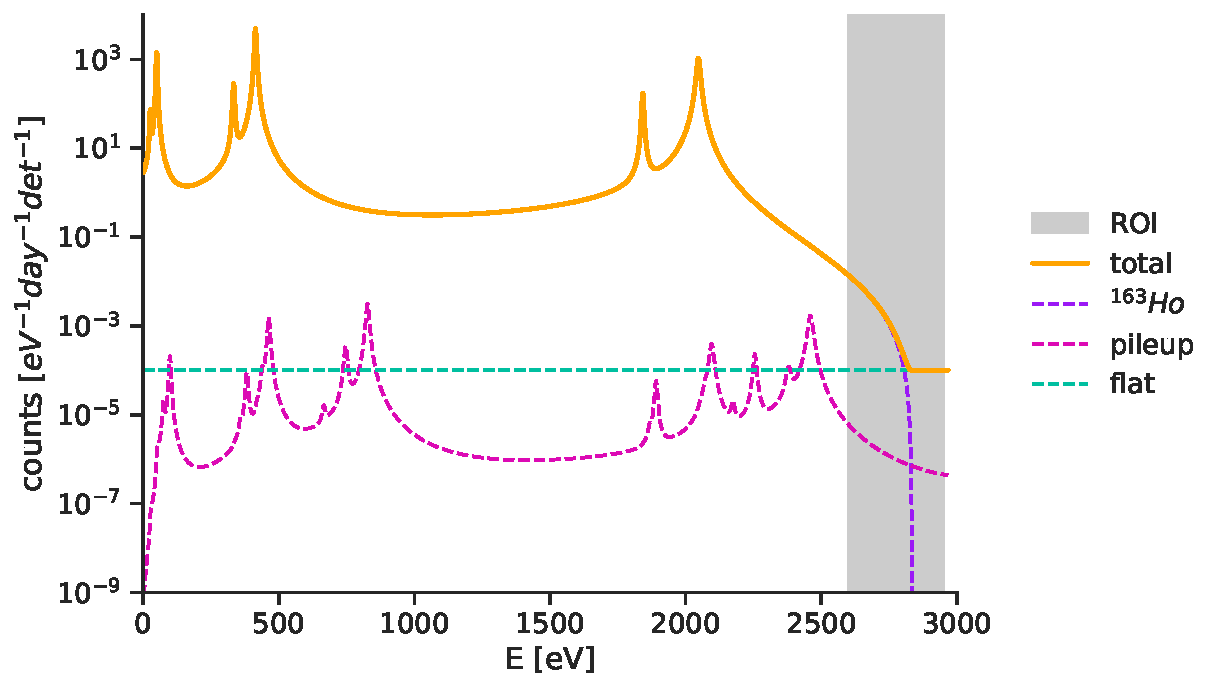
\includegraphics[width=0.85\textwidth]{figures/ch3/spectrum_0.pdf}
  \caption{First-order spectrum with expected flat background and pileup.}
  \label{fig:expected}
\end{figure}
The expected pileup for a certain detector can instead be computed considering its time resolution $\tau_R$ and activity
$A$, with a rough estimate being given by $f_{pp} = \tau_RA$. This estimate can be improved by also considering the pulse
length $L$. Given an energy ROI$=[E_{min}, E_{max}]$, the expected fraction of pileup $f_{pp}$ is computed from 
the probability of events containing a single pulse $P_s$ and that of events containing an additional pulse in
the first $\tau_R$ microseconds from the beginning of the signal ($P_{d}$). The probabilities are weighted by the
integral
of the spectrum and pileup spectrum in the ROI:
\begin{eqnarray}
f_{pp} &=& \frac{P_d}{P_s}\\
P_d &=& \text{Poisson}(1 \mid \tau_R \times A) \int_{E_{min}}^{E_{max}} S(E) * S(E) dE\\
P_s &=& \text{Poisson}(0 \mid L \times A) \int_{E_{min}}^{E_{max}} S(E) dE
\end{eqnarray}
While without further elaboration the time resolution coincides with the sampling time of the signal, with the
application of filtering techniques and cuts it is possible to reduce it by a factor of two. For the current
configuration $\tau_R = 2 \mu$s, while $L = 4$ ms. Considering an activity of $\sim 1$ Bq, this results in an expected
pileup fraction $f_{pp} \sim 2 \times 10^{-6}$ over the whole spectrum. The first-order spectrum with the expected
background is shown in Fig \ref{fig:expected}.



\section{Spectrum characterization}
\subsection{Acquired data}
This section presents the analysis of data obtained during a characterization run using a calibration source and the
experimental setup
described in Sec \ref{sec:setup}. The data was collected from the array implanted with a single central spot
of $^{163}$Ho. Out of the 64 detectors in the array, 54 provided consistent readings, while the others were discarded
due to various detector imperfections, such as defective resonators on the $\mu$MUX chip.

The resulting activity map, shown in Figure \ref{fig:data} (a), represents the event rate in each detector. While the
profile of the beam used for implanting the isotope doesn't appear to be gaussian, the higher activity at the center of
the array indicates proper alignment. However, the observed activity of $^{163}$Ho in the central detectors seems to be three times lower than expected.

Though the activity is too low to study the spectrum endpoint within a reasonable time, this setup is suitable for
characterizing the rest of the spectrum. Figure \ref{fig:data} (b) shows a spectrum obtained
by combining data from four detectors. Besides the four main peaks of the first-order spectrum, additional features can be
observed, such as second-order peaks after M1, and an asymmetric slope in the broad region between N1 and M2. The peak
at around 1500 eV corresponds to the K$_\alpha$ line of aluminum in the calibration source.

The observed energy resolution for all detectors ranges between 5 and 10 eV, with a mean NEP estimate of $7.3\pm 1.3$ eV. However, comparing the acquired spectra
reveals systematic effects introduced during the data processing, altering the measured energy in each detector, as
depicted in Figure \ref{fig:data} (c). While these systematics will require further investigation, in this thesis they
will be treated as an overall energy shift in each detector's response.

This analysis focuses on the M1 peak, which is of particular interest for neutrino mass estimation as it is the closest
to the endpoint. The Region of Interest is chosen to be between 1950 eV and 2150 eV. Only data from the 16 detectors
with the highest activity is considered, resulting in approximately 161,000 events in the ROI, with each detector having
measured between 1600 and 25,500 pulses.

Considering both natural radioactivity and pileup, the total fraction of background events in the ROI is expected to
be around $10^{-6}$ for the detector with the highest activity and approximately $1.5 \times 10^{-5}$ for the detector
with the lowest. Since the expected number of background events in each detector is less than one, background effects
can be safely neglected in the following analysis.

\begin{figure}[t]
\begin{subfigure}[b]{0.45\linewidth}
  \hfill
  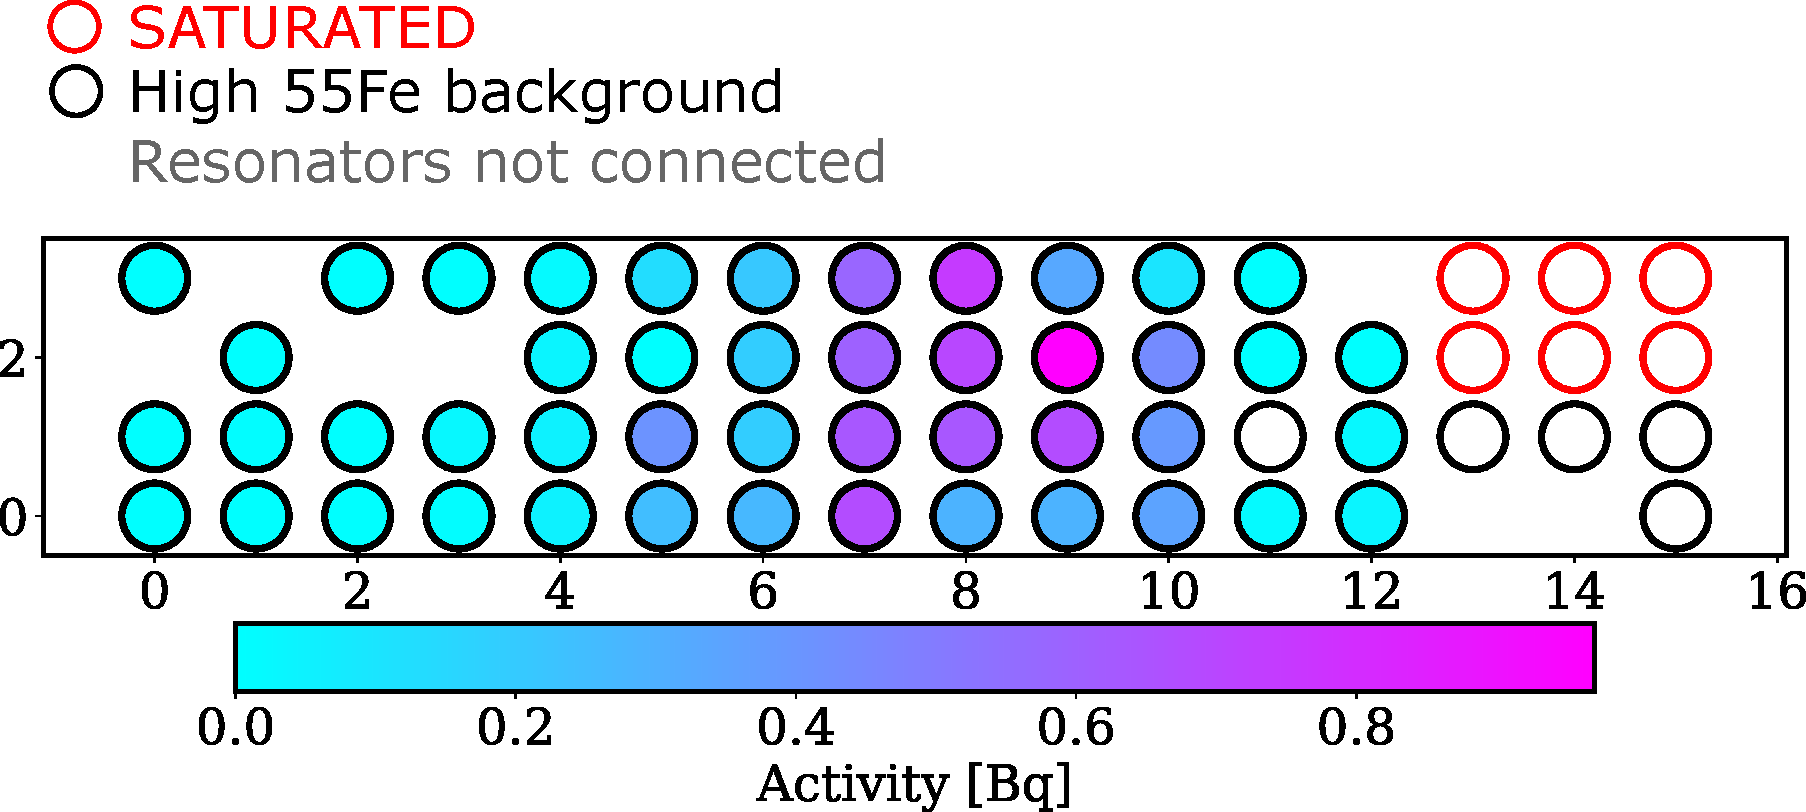
\includegraphics[width=\linewidth]{figures/ch3/activity_tesA.pdf}
  \hfill
  \caption{}
\end{subfigure}
\begin{subfigure}[b]{0.55\linewidth}
  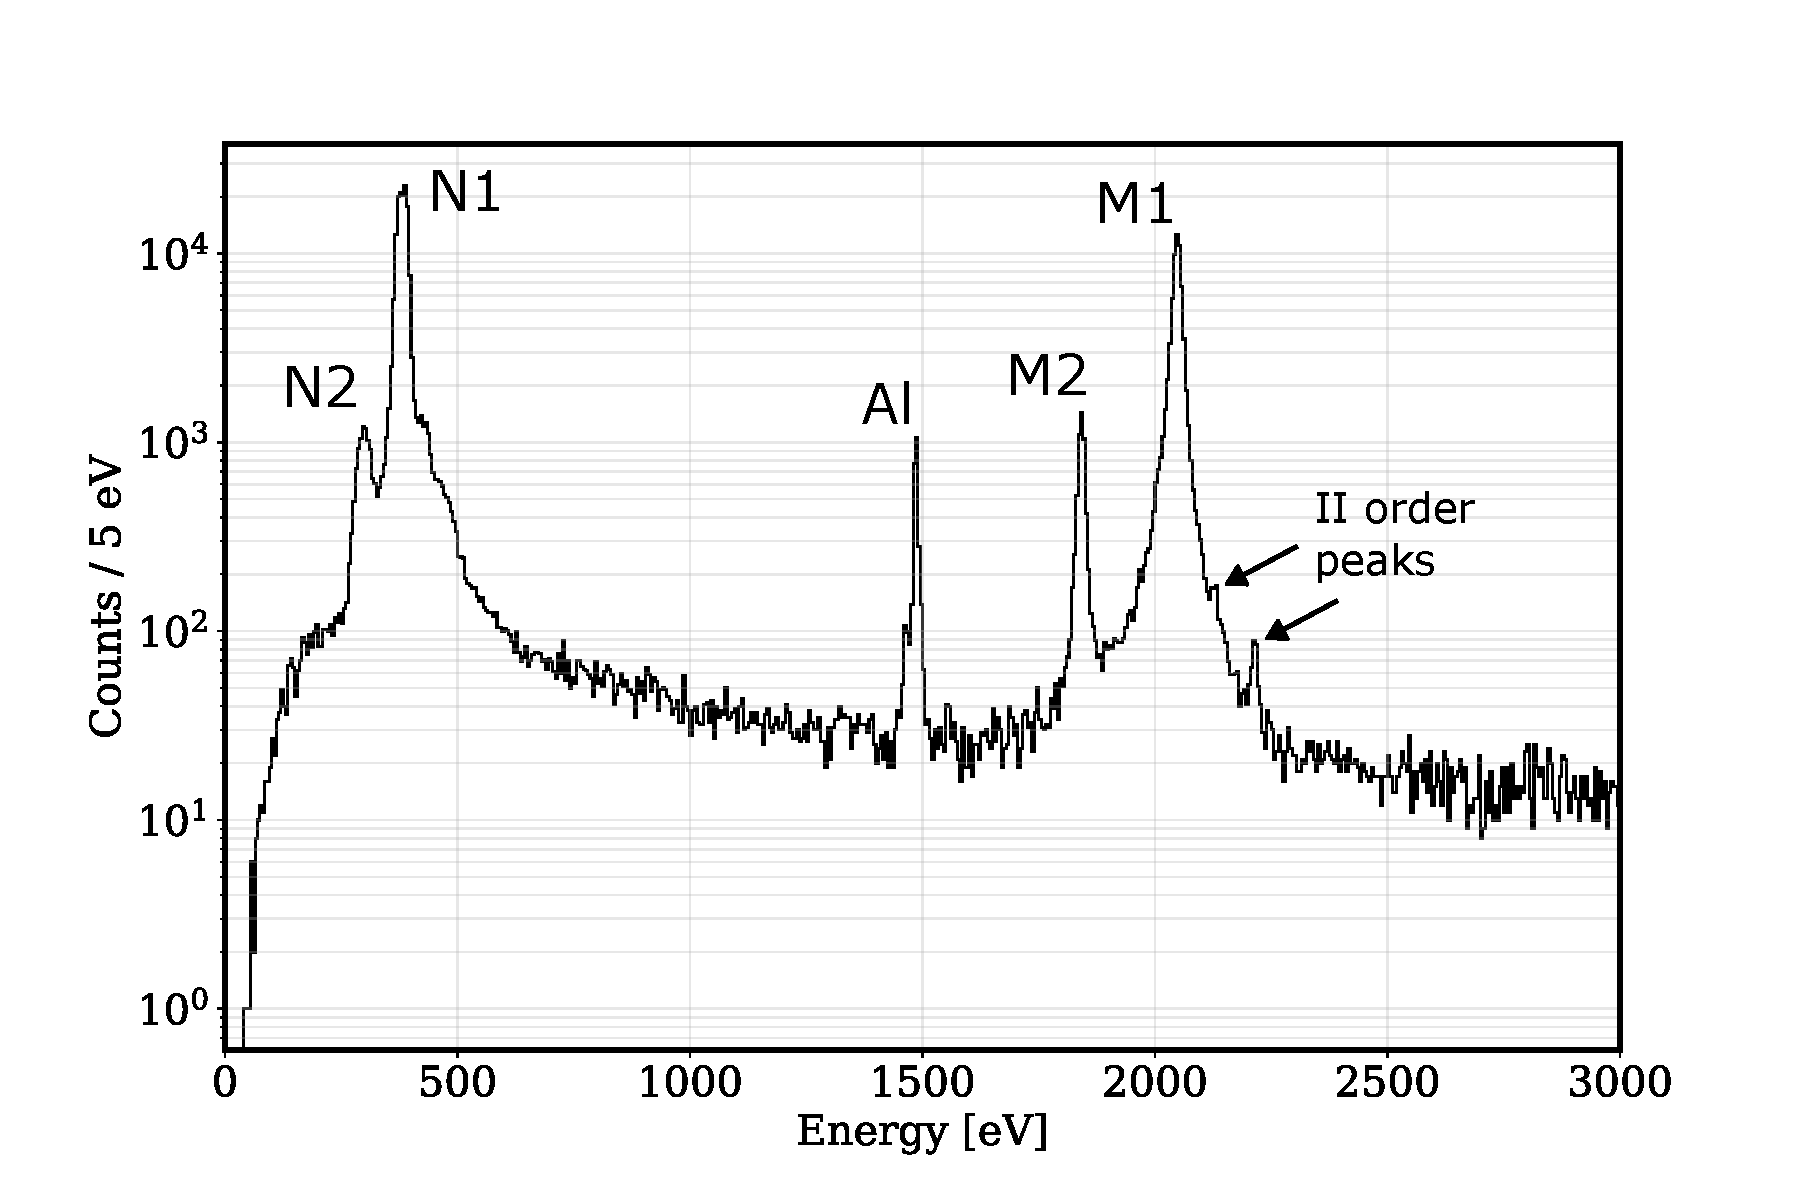
\includegraphics[width=\linewidth]{figures/ch3/Ho_combined.pdf}
  \caption{}
\end{subfigure}
\begin{minipage}{\textwidth}
\begin{subfigure}[b]{\linewidth}
  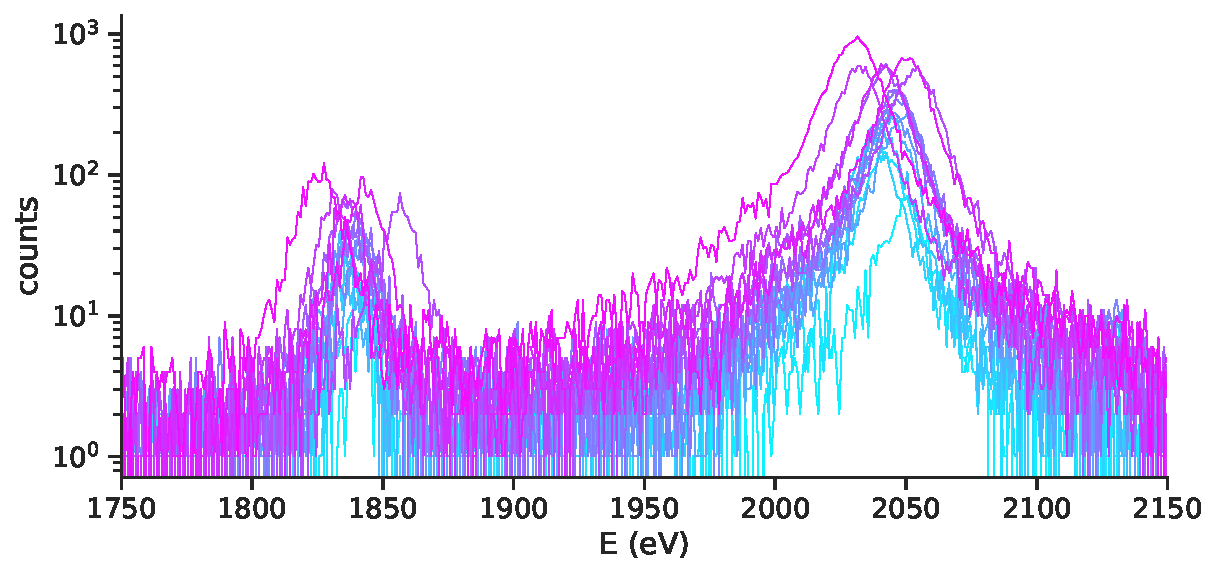
\includegraphics[width=\linewidth]{figures/ch3/peaks/M1M2_0.pdf}
  \caption{} 
\end{subfigure}
\end{minipage}
\caption{Activity map of the 64 TES array in the initial measurement of Holmes (a). First acquired $^{163}$Ho spectrum obtained by
combining data from 4 TESs (b). Focus on the M1 and M2 region of the spectrum acquired by the 16 detectors with the
highest activity. Systematics in the energy calibration shift the observed spectrum differently for each detector (c).}
\label{fig:data}
\end{figure}


\subsection{Single detector model}
To begin, a single detector is considered and approximate function is used to fit the observed M1 peak, with the aim to
characterize its main parameters: the position $E_{M 1}$ and width $\Gamma_{M 1}$.
The underlying peak is therefore described by a Lorentzian summed to a first-order polynomial, which approximates the
other features in the spectrum, multiplied by the phase space of Eq \ref{eq:hofirstorder}:

\begin{equation}
  S(E)= [L(E, E_{M 1}, \Gamma_{M 1}) + m(E-E_0) + y_0)]\times PS(E, Q, m_\nu)
\end{equation}

In this equation, $L$ is the Lorentzian representing the M1 peak, while the polynomial is constructed relative to the initial point $E_0$ of the
ROI. For the phase-space term $PS$, a neutrino mass of 0 eV and  $Q=2833$ eV will be assumed in the following
analysis. To obtain the experimental spectrum $S_{\exp}(E)$, $S(E)$ is convolved with a gaussian function of width
$FWHM$ representing the resolution of the detector. The resulting spectrum is normalized to 1 in the ROI.

The basic model used for this fit includes the following free parameters: the peak position $E_{M1}$, its width $\Gamma_{M1}$, the
intercept $y_0$ and slope $m$ of the polynomial, the
energy resolution of the detector $FWHM$, and an overall normalization factor $A$ to account for fluctuations of the observed number of events $N_{tot}$ in the ROI. 
The fit is performed by binning the data with a bin width of 1 eV and assuming Poisson fluctuations for the number of
events $N_{ev}[i]$ in each bin. The convolution operation between the theoretical spectrum and the Gaussian experimental
response is handled carefully to avoid border effects. The spectrum is initially computed over a wider range, determined
by the width of the Gaussian response, and then trimmed down to the ROI. Additionally, a convolution function using the
Fast Fourier Transform (FFT) is implemented in Stan to improve efficiency.


The model's priors constrain the parameters within their expected ranges. The resonance position $E_{M1}$ follows a
weakly regularizing prior given by a normal distribution centered on the expected value from the first-order approximation
($E_{M1}^{th} = 2047$ eV) and with a standard deviation of 50 eV. Similarly, $\Gamma$ has a Gamma prior centered on 13.2 eV,
with 90\% of the probability mass between 5 and 25 eV. The prior for $FWHM$ considers the estimate given by the NEP as
a lower bound. Since the NEP is usually obtained with $\pm 0.2$ eV precision, the Frechet distribution is used to construct a prior with 99\% of the probability falling between $NEP-0.4$ eV and $NEP+4$ eV. The normalization factor $A$ is
considered to vary around 1 with a normal standard deviation of 0.05. Finally, the intercept and slope of the polynomial are
given very tight normal priors in order to prevent the overall spectrum from becoming negative in some points:
\begin{figure}[t]
\begin{subfigure}[b]{0.45\linewidth}
    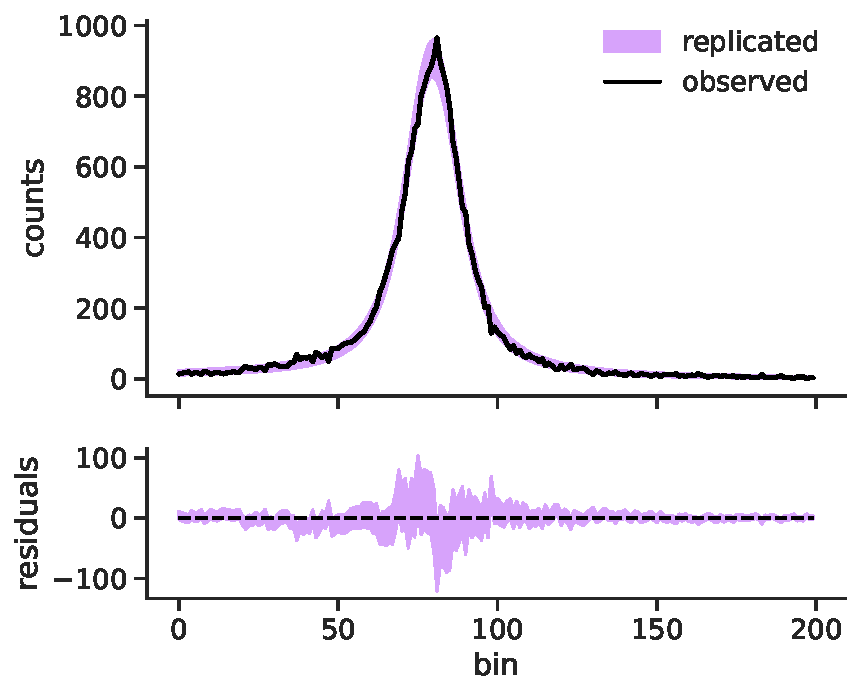
\includegraphics[width=\linewidth]{figures/ch3/peaks/predictive_check_1.pdf}
\caption{}
\end{subfigure}
\hfill
    \begin{subfigure}[b]{0.45\linewidth}
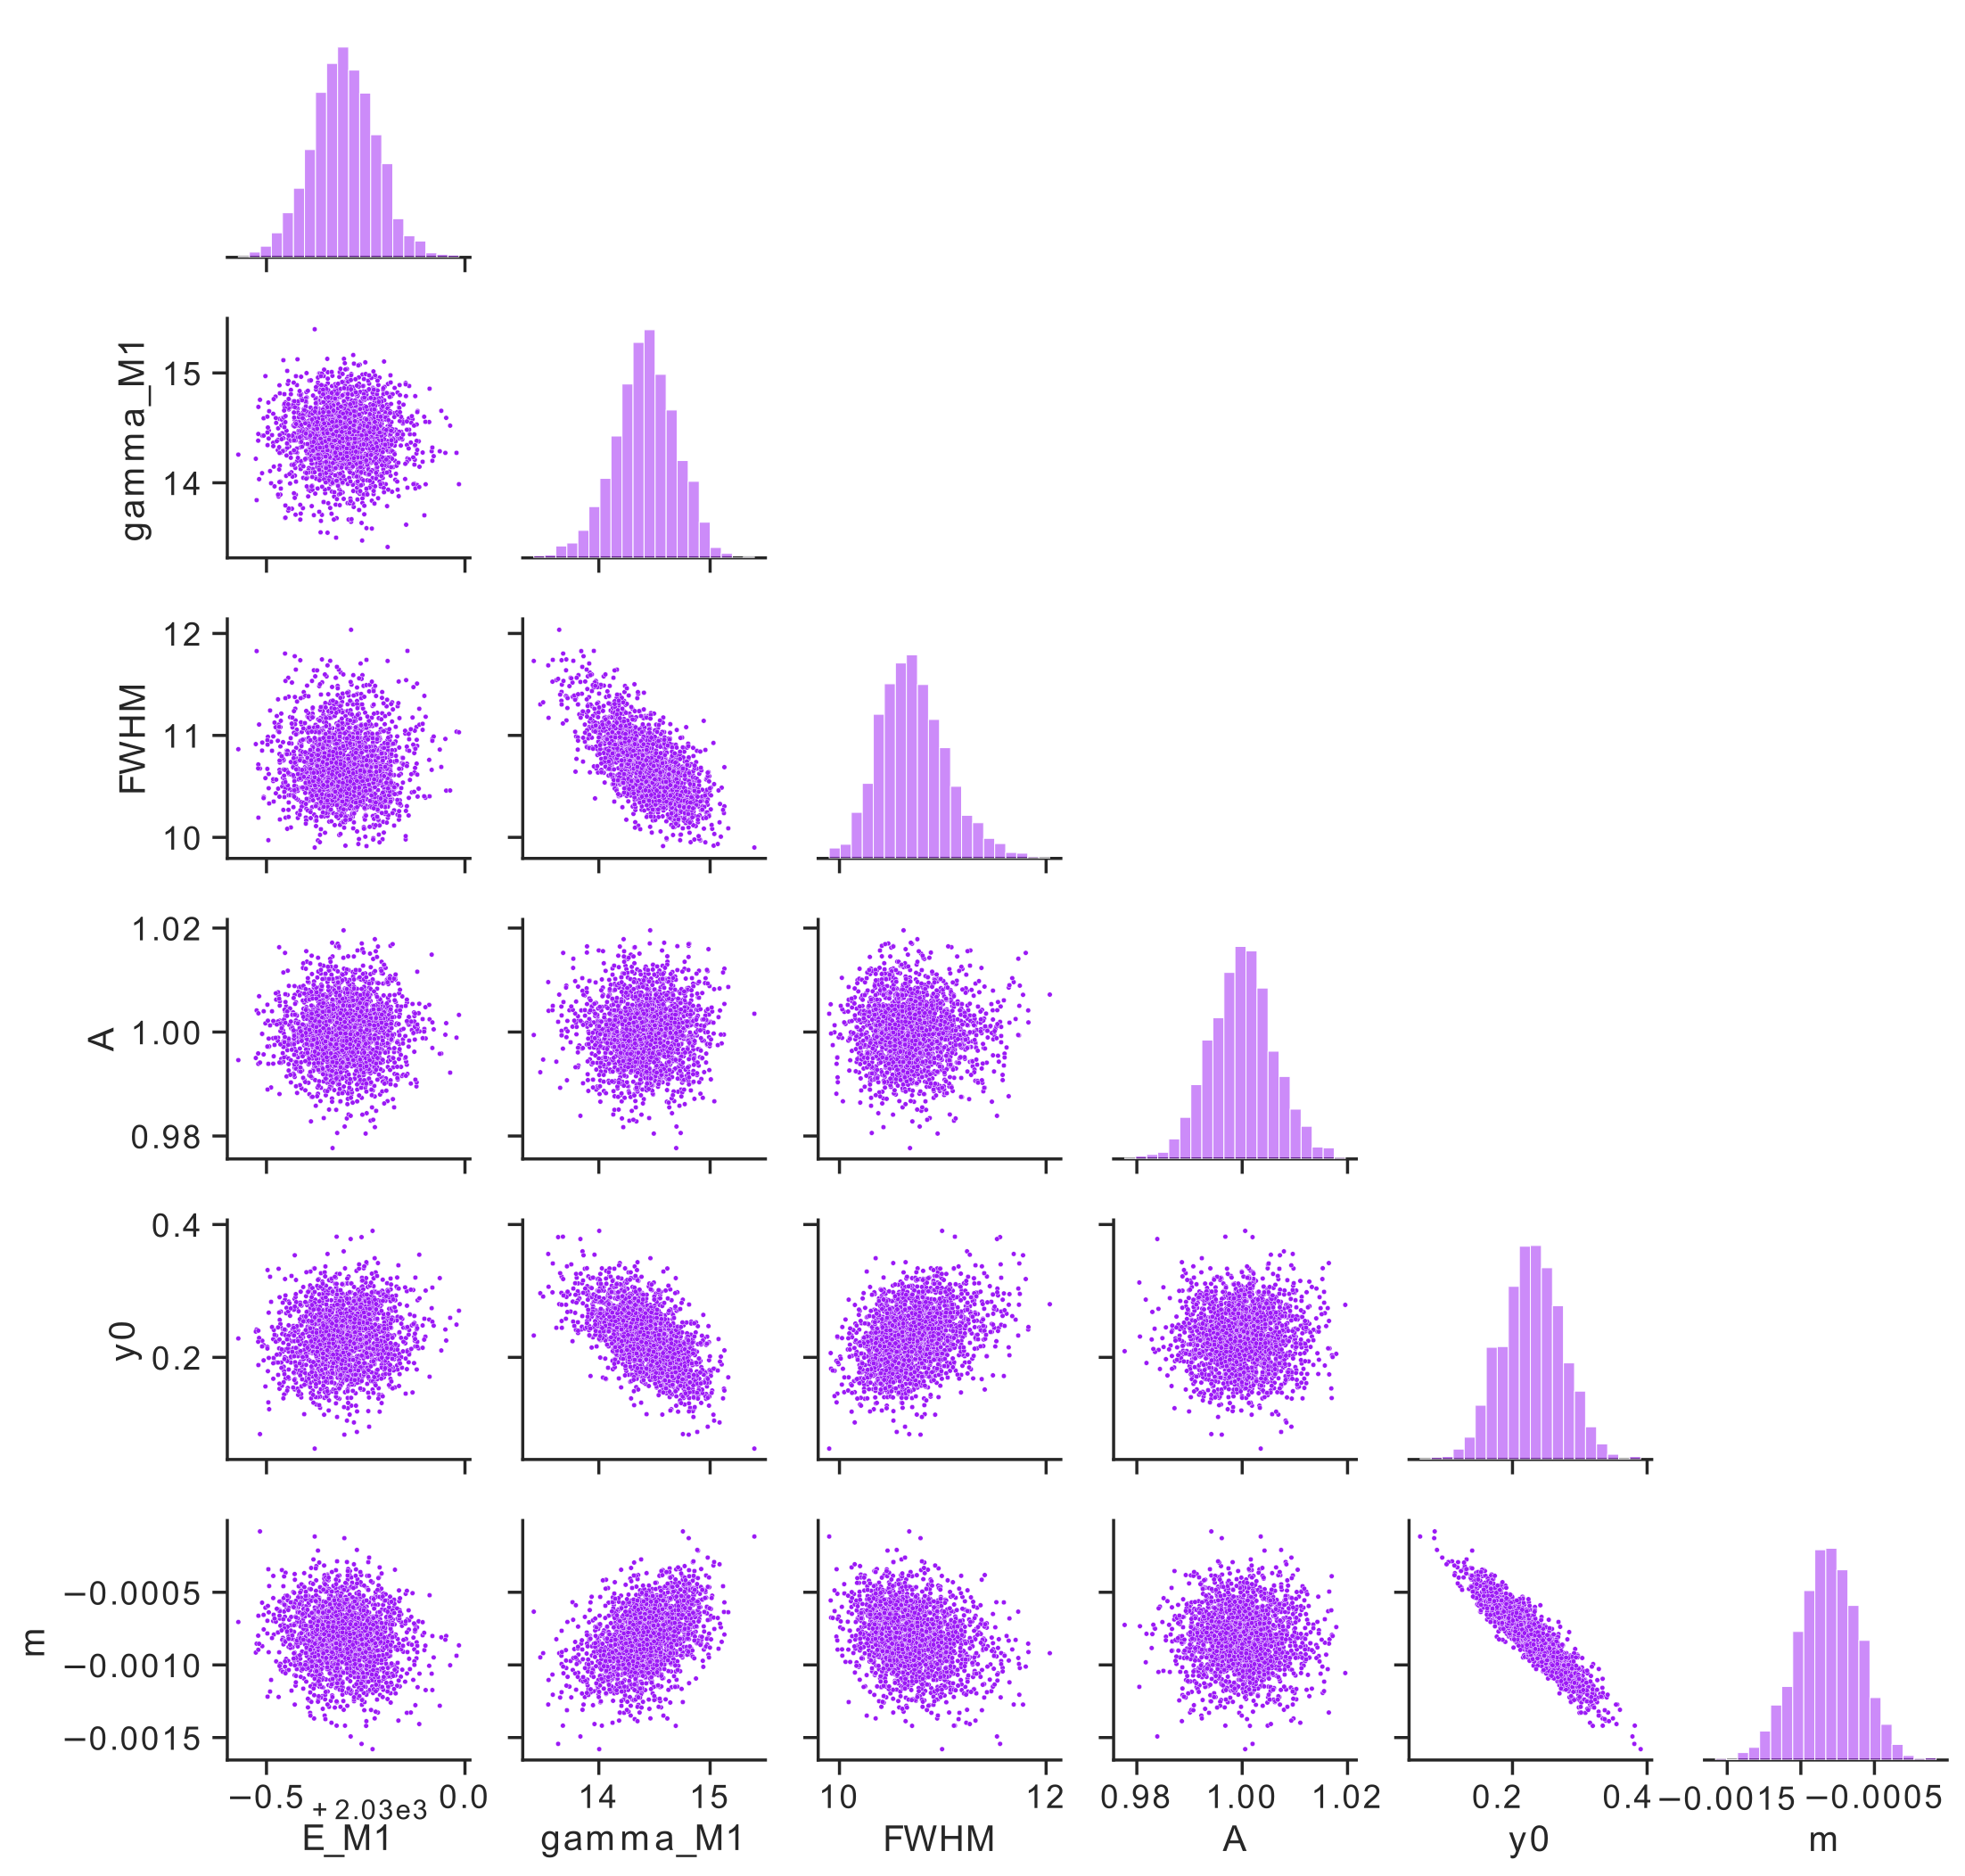
\includegraphics[width=\linewidth]{figures/ch3/peaks/pair_grid_0.png}
\caption{}
\end{subfigure}
\caption{Posterior predictive check for the simple M1 peak model, note the asimmetry of the residuals around the peak (a). Correlations between parameters in the posterior of
the model (b). Data taken from the detector with highest statistics, corresponding to 25500 events in the ROI and
$FWHM=10.5$ eV.} 
\label{fig:peakcorr}
\end{figure}
\begin{eqnarray}
  E_{M 1} &\sim& \text{normal}(2047, 50)\\
  \Gamma_{M 1} &\sim& \text{gamma}(6.6, 0.5)\\
  y_0 &\sim& \text{normal}(0,0.02)\\
  m &\sim& \text{normal}(0,0.01)\\
  FWHM &\sim& \text{frechet}(2\times NEP, \;NEP+0.5)\\
  A&\sim& \text{normal}(1, 0.05)\\
  N_{ev}&\sim& \text{poisson}(S_{\exp}(E, E_{M 1}, \Gamma_{M 1}, y_0, m, FWHM)\times A\times N_{tot})
\end{eqnarray}





The model is efficient, completing the warm-up phase and generating 1000 samples from each Markov chain in less than 10
seconds. Stan's diagnostics do not raise any warnings regarding potential issues, and all the posteriors of the
parameters are narrower than their priors. Figure \ref{fig:peakcorr} presents the
posterior predictive check and correlations between the parameters. While some strong correlations are observed, they do
not introduce significant curvature in the posterior's geometry, and Stan appropriately accounts for them by adjusting
the HMC metric. However, the residuals in the posterior predictive check suggest that the model does not perfectly describe the data. Notably, the residuals appear mostly positive on one side of the peak and mostly negative on the other, possibly indicating a slight asymmetry.

\begin{figure}[t]
  \centering
  \begin{minipage}{0.45\linewidth}
    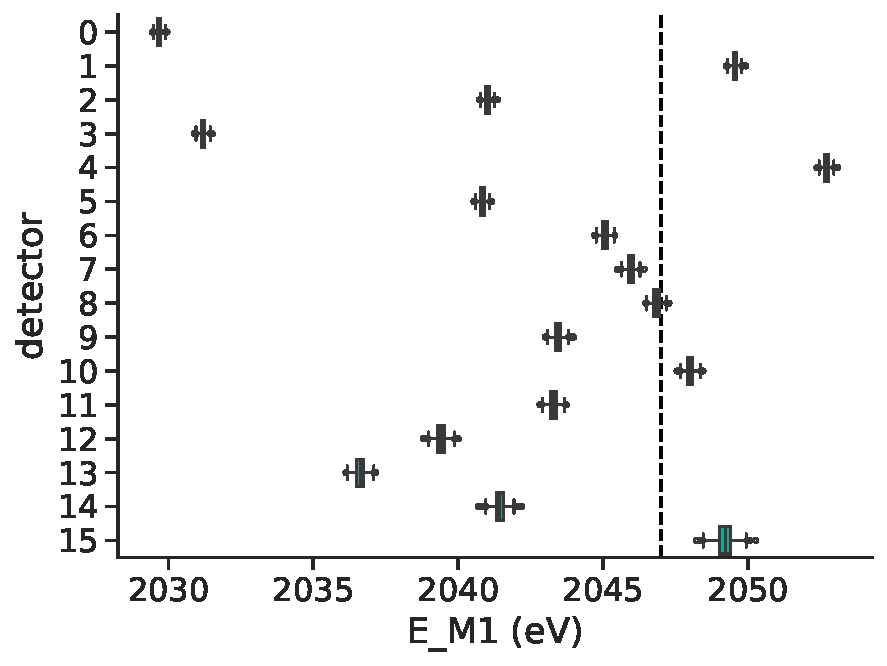
\includegraphics[width=\linewidth]{figures/ch3/peaks/cat_plot_0.pdf}
  \end{minipage}
  \centering
  \begin{minipage}{0.45\linewidth}
    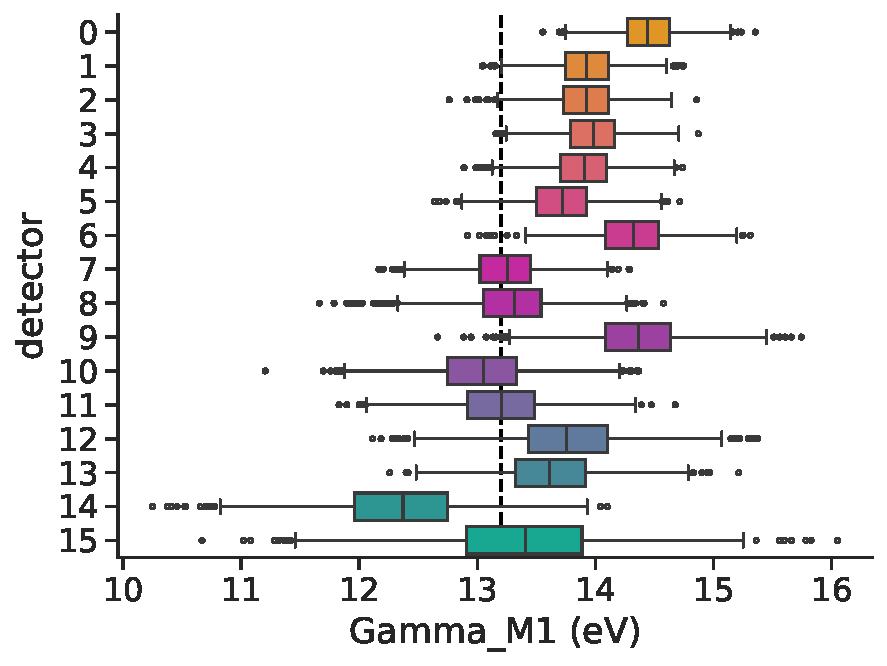
\includegraphics[width=\linewidth]{figures/ch3/peaks/cat_plot_1.pdf}
  \end{minipage}
 % \begin{minipage}{0.33\linewidth}
 %   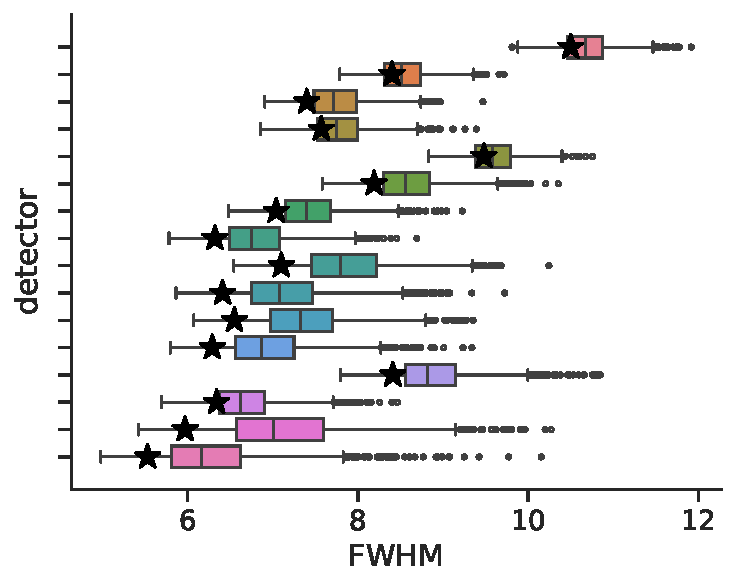
\includegraphics[width=\linewidth]{figures/ch3/peaks/cat_plot_2.pdf}
 % \end{minipage}
 % \hfill
 % \begin{minipage}{0.33\linewidth}
 %   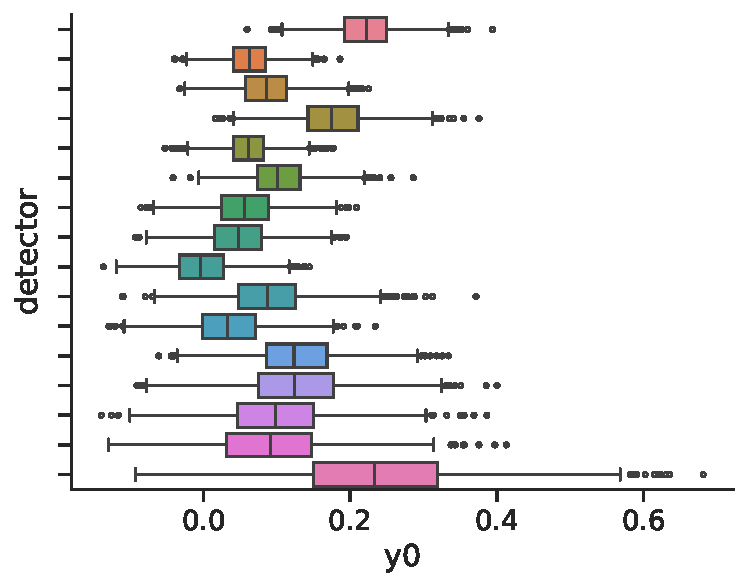
\includegraphics[width=\linewidth]{figures/ch3/peaks/cat_plot_4.pdf}
 % \end{minipage}
 % \begin{minipage}{0.33\linewidth}
 %   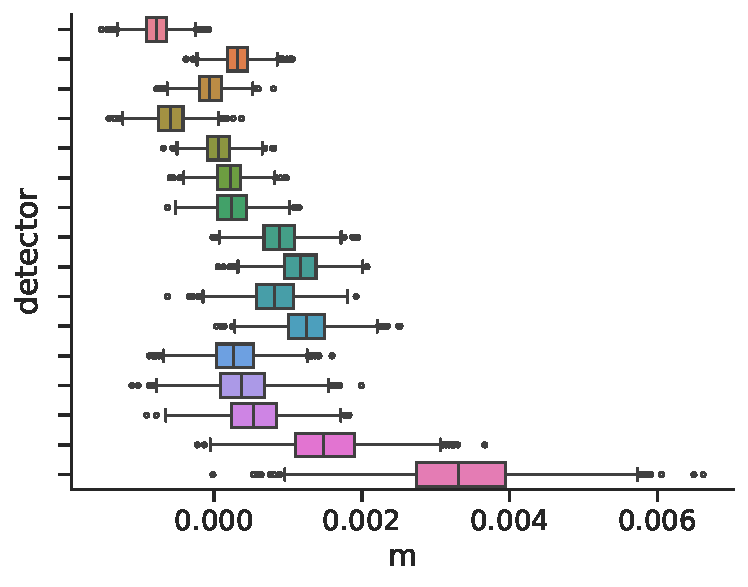
\includegraphics[width=\linewidth]{figures/ch3/peaks/cat_plot_5.pdf}
 % \end{minipage}
 % \begin{minipage}{0.33\linewidth}
 %   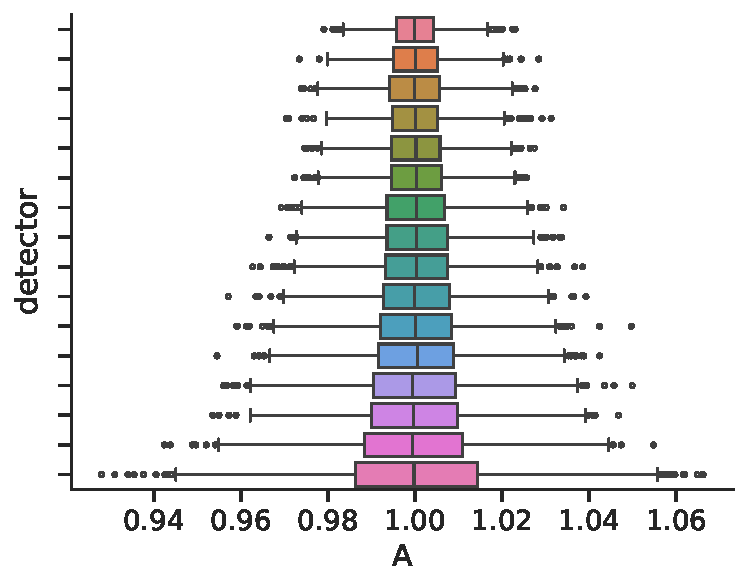
\includegraphics[width=\linewidth]{figures/ch3/peaks/cat_plot_3.pdf}
 % \end{minipage}
\caption{Posterior boxplots of independent fits of the M1 peak for 16 detectors, ordered by acquired statistics. The
black lines correspond to the first-order predictions}%, while the blackstars in the graph for $FWHM$ represent the expected energy resolution computed with the NEP.}
\label{fig:singlepeak}
\end{figure}
The fit has been independently repeated for all 16 considered detectors. The resulting posterior distributions for the two
parameters of the M1 peak
are shown in Figure \ref{fig:singlepeak}, with detectors ordered by acquired statistics, from highest (1) to
lowest (16). In each case, a value for $E_{M 1}$ identified with an accuracy of approximately 1 eV. However, due to the calibration
systematics this results in significantly different predictions for various detectors. On the other hand, results are more
consistent for the peak width, though they tend to be slightly higher than the first-order
prediction. The $FWHM$ of all detectors are found to be not more than 1 eV higher than the NEP estimate. A slightly positive slope and intercept of the polynomial is found in most cases,
while the normalization factor $A$ is tightly constrained around 1 due to the
relatively high statistics. 

\subsection{Lineshape asymmetry}
Higher order predictions introduce additional peaks in the spectrum and reveal an asymmetric broadening of resonances caused by Auger-Meitner decays. The latter phenomenon
involves the transfer of energy from an electron filling a vacant orbital created in the EC decay to
another electron, which is ejected from the atom into the continuum, contributing to what is known as the shake-off spectrum. These predictions, along with the observed
deviations in the residuals of the posterior predictive checks, highlight the need to model the M1 peak differently, taking into account a possible asymmetry due to unresolved additional peaks and shake-off.

%In previous studies using data from Echo, it was found that the broadening of the spectrum is consistent with a Mahan lineshape. While this approach is theoretically motivated, it is computationally demanding. Given that the rest of the spectrum is already approximated at the first-order, it is more practical to explore alternative descriptive models with lower computational overhead.

The first model, which will be denoted as LR asymmetry, constructs an asymmetric profile by combining two Lorentzian
distributions with different widths on either side of $E_{M1}$. These widths are defined as $\Gamma_L = (1-a)\Gamma_{M1}
$ and $\Gamma_R = (1+a)\Gamma_{M1}$, where $a$ represents the asymmetry parameter:
\begin{equation}
\text{Lorentzian}_{LR} \propto
\begin{cases}
L(E, E_{M1}, \Gamma_R) \quad \text{for} \quad E \geq E_{M1} \\
L(E, E_{M1}, \Gamma_L) \quad \text{for} \quad E < E_{M1}
\end{cases}
\end{equation}



\begin{figure}[t]
  \centering
  \includegraphics[width=0.87\textwidth]{figures/ch3/peaks/compred_0.pdf}
  \caption{Posterior predictive checks median and 95\% HDI comparing the symmetric and sigmoid width model with both $\alpha$
  and $\beta$. A slight asymmetry is visible in the tails of the M1 peak. Data taken from detector 5, corresponding to
15000 events in the ROI and $FWHM=7.5$ eV.}
  \label{fig:pred_asymm}
\end{figure}

Another approach to introduce asymmetry in the lineshape is to make the peak widths dependent on energy. Recent research \cite{schmid2014new} in characterizing X-ray photoelectric peaks has shown that using a sigmoid function to model the width accurately fits many experimental lineshapes. However, this introduces two additional parameters into the fit:
\begin{equation}
\Gamma_{M1} \rightarrow \Gamma(z, \Gamma_{M1}, \alpha, \beta) = \frac{2\Gamma_{M1}}{1+\exp(-\alpha(x-\beta))}
\end{equation}
Where $x = E - E_{M1}$. The parameter $\alpha$ controls the strenght of the asymmetry, while $\beta$ allows for
shifting from the center of the peak the point where the width changes. These new parameters
are added to the previous model with weak priors. Both $a$ for the LR and $\alpha$ for the sigmoid asymmetry model are limited to the
range of -0.5 to 0.5. For the second model, $\beta$ follows a normal distribution with a standard deviation of 15 eV, centered on 0 eV.
Both models converge without generating warnings. The predictive checks for the symmetric and the full sigmoid model are
shown in Figure \ref{fig:pred_asymm}. While significantly different results do not appear for all detectors, for some of
those with higher statistics the
posteriors for $\alpha$ are notably shifted away from 0, being centered around approximately $-0.01 \pm 0.003$. However,
the posterior for $\beta$ remains unchanged from the prior, even when broad priors are used.

This leads to consider whether to exclude the $\beta$ parameter from the sigmoid model to further reduce computational
overhead. Model comparison has been performed with Leave-One-Out Cross-Validation (LOOCV) to assess the predictive
performance of these three alternatives compared to the basic model with a symmetric Lorentzian. The resulting
estimates of the difference in expected log predictive density (elpd) from the symmetric profile are shown in Figure
\ref{fig:comp}.

In this case, the elpd difference is considered to allow visualizing the comparison across all detectors.
Additionally, the absolute elpd scores have relatively large standard errors, while the errors on the differences
are much smaller due to the absolute estimates being correlated.


\begin{figure}[t]
  \centering
  \includegraphics[width=0.75\textwidth]{figures/ch3/peaks/loooCV_0.pdf}
  \caption{Results of model comparison for different asymmetric lineshapes. The elpd difference with respect to the
  model without asimmetries is plotted on the y-axis for each detector. The two models with a sigmoid tend to
perform similarly, while the LR asymmetry model performs almost exaclty as the symmetric profile.}
  \label{fig:comp}
\end{figure}

In standard practice, an elpd difference above 4 can be considered significant if its error is sufficiently low. As
observed, most detectors benefit from the inclusion of the asymmetric profile. For the constructed estimates, the LR model is predicted to perform
almost exactly as the symmetric Lorentzian, with negligible errors, while both of those employing the sigmoid consistently reach higher and identical
elpd scores. Since the
elpd estimates for the model excluding the $\beta$ parameter and the one with both
$\beta$ and $\alpha$ are practically equivalent both in value and error, this leads
to the choice of using the sigmoid profile with only the additional parameter $\alpha$ to describe the shape of the M1
peak.



%, making the difference in predictive performance more significant. This illustrates how LOOCV and model comparison penalize overfitting,



\subsection{Multiple detectors and energy calibration systematics}
As shown in Fig. \ref{fig:singlepeak}, the energy calibration systematics do not allow obtaining compatible independent estimates of $E_{M 1}$ by
considering the detectors separately. In cases such as these, it is often uncertain how to combine the results.
For statistically compatible values it is usually adivised to do so with a weighted mean, considering the standard
deviation of each measurement, while for incompatible values it is otherwise suggested to compute the error on the overall
estimate as the standard deviation of the means. However, in this case the indipendent measurements of
$E_{M 1}$ are incompatible, but it is known that they actually belong to the same underlying parameter.




Instead of performing the fits separately and combining the results in an arbitrary way, it is possible to construct a single model that considers all the detectors
simultaneously and determines their energy calibration systematics and other parameters at the same time as $E _{M 1}$.
While $E_{M 1}$ and the calibration sistematics, denoted as $\delta E$, are clearly extremely correlated, it is still
possible to obtain sensible estimates of both by assuming that the values of $\delta E$ are distributed around zero.
Moreover, these additional parameters can be organized in a hierarchical prior, allowing to exchange information between
the detectors in their estimation. In this case, $\delta E$ is introduced as an overall shift of the energy read by
each detector.

\begin{figure}[t]
  \begin{minipage}{0.55\linewidth}
    \includegraphics[width=\linewidth]{figures/ch3/peaks/dis_plot_0.pdf}
  \end{minipage}
  \hspace{0.3cm}
  \begin{minipage}{0.4\linewidth}
\begin{tabular}{lrr}
\toprule
 & Mean & StdDev \\
\midrule
  $E_{M 1}$ (eV)& 2043.1 & 1.8 \\
$\Gamma_{M 1}$ (eV)& 13.8 & 0.1 \\
$\sigma_E$ (eV)& 6.9 & 1.2 \\
$\alpha$ & $-9.8\times 10^{-3}$ & $0.6\times 10^{-3}$ \\
\bottomrule
\end{tabular}
  \end{minipage}
\caption{Results of the combined fit of 16 detectors using a hierarchical model to account for energy calibration
systematics. The posteriors of the parameters shared by all detectors are plotted on the left, while the table on the
right contains their means and standard deviations.}
\label{fig:preliminaryres}
\end{figure}
This model considers the asimmetric sigmoid lineshape without $\beta$, using $E_{M 1}$, $\Gamma_{ M 1}$, $\alpha$, $y_0$
and $m$ as global parameters to determine the true shape of the M1 peak.
Each detector is also assigned additional parameters for $\delta E$, $A$, and $FWHM$. It is assumed that each $\delta E$ follows a normal distribution around zero with a standard deviation represented by $\sigma_E$, which is the hyperparameter of the hierarchical prior.
$\sigma_E$ represents the expected spread in energy calibration among the detectors and is assigned a Gamma hyperprior centered on 8 eV, covering the range [4, 20 eV].

The likelihood is computed by iterating over the data from each detector, with the i-th detector containing a total of
$N_{tot}[i]$ events distributed across the bins. Considering that the priors of the basic model are used for the global
parameters of the peak, the new model is specified as:
\begin{eqnarray}
  \alpha &\sim& \text{normal}(0,0.15)\\
  \sigma_E &\sim& \text{gamma}(8, 1)\\
  \delta E[i] &\sim& \text{normal}(0, \sigma_E)\\
  FWHM[i] &\sim& \text{frechet}(2\times NEP[i], \;NEP[i]+0.5)\\
  A[i] &\sim& \text{normal}(1, 0.05)\\
  N_{ev}[i] &\sim& \text{poisson}(S_{\exp}(E-\delta E[i], E_{M 1}, \Gamma_{M 1}, \alpha, y_0, m, FWHM[i])\times A[i]
  \times N_{tot}[i])\qquad
\end{eqnarray}
For 16 detectors, the model contains 54 parameters and requires approximately one hour to converge and produce 500
samples from a chain, but no potential problems are identified.
Figure \ref{fig:preliminaryres} shows the posteriors of the parameters shared by all detectors, which constitute
preliminary results for the characterization of the first experimental spectrum acquired by Holmes. 
Both the obtained M1 position 2043.1$\pm 1.8$ eV and the value of $\Gamma_{M 1}=13.8\pm 0.1$ eV are consistent with other
measurements by Echo  \cite{thirdorder} within $2\sigma$ (2040 eV and 13.7 eV respectively), and differ from the first-order theoretical
predictions by some eVs as expected. 
The energy calibration dispersion in the hierarchical prior is estimated to be $\sigma_E = 6.9\pm 1.2$ eV, equivalent to the
standard deviation of the results from separate detectors. Finally, a small but nonero asimmetry is found.
Notably, the asimmetry is negative, meaning that the resonance is slightly wider at lower energies. Since the shake-off
necessarily favors higher energies, the observed asimmetry is probably due to the presence of higher-order peaks in the
M1 profile, with $E<E_{M 1}$, which have not been modeled by using a single Lorentzian.


Figure \ref{fig:systvsM1} compares the posteriors of all $\delta E$ found by the hierarchical model with those
for $E_{M 1}$ obtained by fitting the detectors separately. In order to show the distributions together, each $\delta E$
is shifted by the mean of $E_{M 1}$ found with the hierarchical model, which is plotted along with its 5-95\% credible
interval. As can be seen, the predictions for $\delta E$ are more uncertain than the separate estimates of $E_{M 1}$.
This is due to the fact that they are correlated with the global $E_{M 1}$ in the fit, and their variability reflects
that of the posterior for $E_{M 1}$. However, while the parameters of the single detectors are more uncertain in the
hierarchical model than in the separate fits, in the first all of them concurr to infer the values of the global parameters more precisely, resulting in a better estimate of
$E_{M 1}$ than the one given by the average and standard deviation of the means from separate fits $E_{M1}^{\text{sep}}=2043.2\pm
6.2$ eV.

\begin{figure}[t]
  \centering
  \includegraphics[width=0.9\textwidth]{figures/ch3/peaks/compare_0.pdf}
  \caption{Comparison between separate fits of the data from 16 detector and a single fit of a hierarchical model
  considering the energy sistematics $\delta E$.}
  \label{fig:systvsM1}
\end{figure}

\section{Expected neutrino mass limit}

\subsection{Data generation}

The current experimental data doesn't allow to provide a meaningful limit on the neutrino mass, since all completed and
processed measurements so far used calibration sources that obscure the endpoint region. This section of the thesis
aims to estimate the upper limit on the electronic neutrino mass achievable by Holmes in the near future using its current setup and an array implanted with a low dose of $^{163}$Ho. 
In Bayesian data analysis, the upper limit of a parameter is determined by the quantile of its posterior corresponding
to a certain credibility $\alpha$. Because of this, the limit $m_{\text{lim}}$ for $m_\nu$ will be calculated as:
\begin{equation}
\int_0^{m_{\text{lim}}} dm_\nu p(m_\nu\mid y) = 1-\alpha
\end{equation}
where $p(m_\nu\mid y)$ represents the marginal posterior of $m_\nu$.

To simulate the results of a measurement campaign, fake energy spectrum data are generated using Monte Carlo simulation
and then fitted. Since the shape of the endpoint doesn't appear to strongly depend on the rest of the spectrum, which
will be thoroughly characterized in the upcoming measurements of Holmes, the simulated dataset is generated
considering as a theoretical model the first-order spectrum. Finite energy resolution, background, and pile-up are then added.


Starting from the first-order spectrum $S(E)$ with fixed parameters, the experimental spectrum used for data generation
and fitting is given by:

\begin{equation}
S_{\text{exp}}(E) = [(1-f_{\text{pp}}-f_{\text{bkg}})S(E) + f_{\text{pp}} S(E) * S(E)+ f_{\text{bkg}}] * \text{Normal}(0, \text{FWHM})
\end{equation}

This spectrum is then binned and normalized in the ROI. A new dataset is generated by fluctuating the spectrum according to Poisson statistics, with a rate of $S_{\text{exp}}(E)\times A_{Ho}\times N_{\text{days}}$ in every bin. 
\begin{figure}
  \begin{minipage}{0.55\linewidth}
    \includegraphics[width=\linewidth]{figures/ch3/endpoint/generated_0.pdf}
  \end{minipage}
  \hfill
  \centering
  \begin{minipage}{0.4\linewidth}
    \begin{tabular}{l r} \hline 
      \toprule
         Parameter & Value\\
         \midrule
         $m_\nu$& 0 eV\\
         Q& 2833 eV\\
         $A_{Ho}$& 1 Bq\\ 
         $N_{days}$& 100\\
         $N_{det}$& 64\\
         $FWHM$& 7 eV\\
         ROI& 2600-2950 eV\\ 
         \bottomrule
    \end{tabular}
  \end{minipage}
\caption{Example of simulated spectrum combining the observations of 64 identical detectors. The table shows the
parameters used for the simulation.}
\label{fig:simdata}
\end{figure}

This analysis will focus on a possible near-term measurement campaign with a baseline of 64 detectors implanted with $A_{Ho}\sim1$ Bq each, resulting in approximately 5900 events in the ROI, defined to be between 2600 eV and 2950 eV. An example of simulated data and the corresponding parameters are shown in Fig \ref{fig:simdata}.


According to the estimates of Sec \ref{sec:expected}, the expected fraction of background events in the ROI
due to radioactivity and cosmic rays is $f_{\text{bkg}}\sim 3\%$, while the pileup fraction is $f_{\text{pp}}\sim
5\times 10^{-4}$. The pileup spectrum in the ROI only weakly depends on $Q$ and $m$, which are the main free parameters
in this analysis. Furthermore, the flat background is more than 15 times higher than the pileup at every point in the
ROI, and the available statistics do not allow to differentiate between the two, since approximately 2.5 pileup events
are expected in the whole measurement. Therefore, the background will be approximated with a prevalent flat component
summed to a fixed pileup generated from the first-order spectrum, with $f_{\text{pp}}$ set to its expected value.

\subsection{Single detector}

This section discusses the basic model used for analyzing data in the endpoint region. The simulated data assumes that
all the detectors are identical, combining all the observations into a single experimental spectrum as if it originated
from one detector with the compound statistic. 


The model involves five parameters: $m_{\nu}$, $Q$, the fraction of flat background $f_{bkg}$, the energy resolution
$FWHM$, and a normalization factor $A$.
To assess Holmes' sensitivity to $m_{\nu}$, a flat prior ranging from 0 to $m_{max}=$ 300 eV is assigned to $m_{\nu}$.
This constraint ensures that the mass remains positive, while values greater than $m_{max}$ would cause the spectrum
endpoint to fall outside the ROI, rendering inference impossible.
On the other hand, the other parameters can be given more informative priors, since they model the systematics involved
in the experiment. The prior for $Q$ is a gaussian centered on the value obtained with a Penning trap measurement
$Q=2833\pm 30^{stat}\pm 15^{syst}$  \cite{eliseev2015direct}, assuming to
combine the statistic and systematic errors in quadrature. The prior for $f_{bkg}$ is a
Beta distribution with mean $0.06$ and extending between  $0$ and  $0.2$, covering the expected background fraction. The
prior for $FHWM$ is a gaussian with mean and standard deviation corresponding to those of the detectors measured in the
previous section, while $A$ is considered to be normally distributed around 1 with variation  $\pm 5\%$.
The complete model specification is given by:
\begin{eqnarray}
  m_{\nu}&\sim& \text{uniform}(0, 300)\\
  Q &\sim& \text{normal}(2833, 33.5)\\
f_{bkg}&\sim& \text{beta}(1.2,20)\\
FWHM & \sim & \text{normal}(7, 1.2)\\
A &\sim& \text{normal}(1, 0.05)\\
N_{ev} &\sim& \text{poisson}(S_{exp}(E, m_{\nu}, Q, f_{bkg}, FWHM)\times A \times N_{tot})
\end{eqnarray}
Where $N_{tot}$ is the total number of events. The implementation of the model in Stan procedes in the same way as for
the lorenztian peaks, using FFTs to compute the convolution of the binned spectrum with the gaussian energy response.
The posterior predictive check and posterior distributions for the parameters are shown in Fig \ref{fig:endcorr}. 
\begin{figure}[t]
\begin{subfigure}[b]{0.45\linewidth}
    \includegraphics[width=\linewidth]{figures/ch3/endpoint/predictive_check_1.pdf}
\caption{}
\end{subfigure}
\hfill
    \begin{subfigure}[b]{0.54\linewidth}
\includegraphics[width=\linewidth]{figures/ch3/endpoint/pair_grid_0.png}
\caption{}
\end{subfigure}
\caption{Posterior predictive check for the simple endpoint model (a). Correlations between parameters in the posterior of
the model (b).} 
\label{fig:endcorr}
\end{figure}

This model typically requires less than two minutes to generate a chain with around 1000 samples. It can be employed to explore the fundamental interactions between the parameters and assess its robustness in tasks requiring many iterations, such as sensitivity analysis and simulation-based calibration, before extending its scope.

The most notable correlation arises between $m_\nu$ and $Q$, since both parameters determine the endpoint.
 Moreover, the correlation induces a curve that terminates in a sharp corner. Since an
alternative parametrization that uncorrelates $m_\nu$ and $Q$ is difficult to obtain due to the
phase space formula, in this case an informative prior on $Q$ is required not only to otain better inference on  $m_\nu$ but
to avoid divergent transitions. Ideally, part of the measurement could be used to estimate $Q$ better than the value in
the literature and use the result as a more stringent prior. 
Preliminary results from Echo's high-statistics measurements suggest a new estimate of $Q=2837\pm 5^{\text{stat}}\pm
5^{syst}$ eV  \cite{velte2020measurement}. However, using this new value as a prior doesn't appear to significantly alter
the posterior of $m_\nu$.

Another less apparent but important correlation in Fig \ref{fig:endcorr} is the one between $Q$ and  $f_{bkg}$. Being negative, this
correlation hints at the fact that higher background rates limit the ability to accurately measure $Q$ and consequently
$m_\nu$ by covering the
endpoint. However, measuring how
the sensitivity of Holmes changes relative to different overall values of the systematics is beyond the scope of this analysis, which is focused on prior sensitivity. For the latter, the inference on $f_{bkg}$ is robust, allowing to recover the
simulated value of $f_{bkg}$ as long as the priors constrain it to be $<0.2$.

\begin{figure}[t]
\begin{subfigure}[b]{0.5\linewidth}
    \includegraphics[width=\linewidth]{figures/ch3/endpoint/sensitivity_FW_0.pdf}
\caption{}
\end{subfigure}
%\hfill
    \begin{subfigure}[b]{0.5\linewidth}
\includegraphics[width=\linewidth]{figures/ch3/endpoint/sensitivity_0.pdf}
\caption{}
\end{subfigure}
\caption{Results of sensitivity analysis of the simple endpoint model. The experimental resolution doesn't seem to affect
the fit procedure, always resulting in equal priors and posterior for data generated with a fixed $FWHM=7$ eV (a).
Posterior 95\% HDI and median for $m_\nu$ as a function of its prior maximum value $m_{max}$. Values of $m_{max}$ higher
than the relevant scale of the posterior ($\sim 50$ eV) do not affect inference.} 
\label{fig:endsensitivity}
\end{figure}
To investigate whether the problematic correlation between $m_\nu$ and $Q$ introduces biases in the posterior estimation,
the performance of HMC in fitting this model is assessed using Simulation-Based-Calibration.
The results indicate that Stan can correctly sample from the posterior.% However, it's essential to adjust the region of
%interest depending on the simulated value of $m_\nu$ to center it around the endpoint.

Interestingly, when fitting this model, the energy resolution ($FWHM$) does not seem to substantially influence the
results based on the available statistics. There appears to be little information about $FWHM$ that can be extracted
from the data when focusing solely on the ROI. Sensitivity analysis involving resolutions between 1-20 eV reveals that
the posterior for $FWHM$ is essentially the same as its prior distribution, regardless of the true value used to
generate the data (Figure 2a). Moreover, the upper limit on $m_\nu$ remains relatively constant even when considering
prior values of $FWHM$ both higher and lower than that used in data generation. The upper limit on $m_\nu$ only begins to worsen with grossly misspecified priors (e.g., $FWHM_{prior}>20$ eV for data with $FWHM=7$ eV).
Therefore, the $FWHM$ can be constrained with a narrow prior obtained from peak fitting or the NEP estimate, but it
could also be set to a fixed estimate to simplify the model.

Another interesting factor to be tested with sensitivity analysis is the robustness of the posterior of $m_{\nu}$ to the upper
limit of its prior, denoted as $m_{max}$. In fact, some practitioners advise against using flat priors, even when
defined over a finte range, since the posterior can become very dependent to the prior's limits due to the
discontinuities at the edges. This is not the case for this model, as shown in Fig \ref{fig:endsensitivity} (b), where the
posterior of $m_\nu$ doesn't seem to be influenced from the prior after $m_{max}>50$ eV.%, as would be expected from the 90\%

%\begin{figure}[h]
%    \begin{subfigure}[b]{0.24\linewidth}
%\includegraphics[width=\linewidth]{figures/ch3/endpoint/SBC_0.pdf}
%\end{subfigure}
%\begin{subfigure}[b]{0.24\linewidth}
%    \includegraphics[width=\linewidth]{figures/ch3/endpoint/SBC_1.pdf}
%\end{subfigure}
%\label{}
%    \begin{subfigure}[b]{0.24\linewidth}
%\includegraphics[width=\linewidth]{figures/ch3/endpoint/SBC_2.pdf}
%\end{subfigure}
%\begin{subfigure}[b]{0.24\linewidth}
%    \includegraphics[width=\linewidth]{figures/ch3/endpoint/SBC_3.pdf}
%\end{subfigure}
%\caption{Results of SBC for the simple endpoint model, shown as the ECDF of the ranks for each variable.}
%\label{fig:endSBC}
%
%\end{figure}

\subsection{Deriving a robust limit}


By repeatedly fitting datasets generated with the same parameters, it becomes apparent that the
resulting posterior distributions can vary (Fig \ref{fig:endmany}). These variations cannot be attributed to the initial
Markov Chain starting point, the random number generator of the Markov Chain, or instability due to extreme sensitivity
to a prior. Instead, they seem to arise from inherent fluctuations within the data. This can be explained by the fact
that for the low overall number of collected events it is possible to obtain data with less counts than expected
exactly at the endpoint, appearing as if the neutrino mass were significantly different from zero. These fluctuations
are quite rare, appearing only in one simulation every 20, but they still present a source of additional uncertainty in
predictions based on simulated data.
\begin{figure}[b]
  \centering
  \includegraphics[width=0.8\textwidth]{figures/ch3/endpoint/cat_plot_0.pdf}
  \caption{Boxplots of 100 posteriors for $m_{\nu}$, each obtained from data simulated with the same parameters.}
  \label{fig:endmany}
\end{figure}

In cases where these fluctuations are significative, it becomes important to account for them to derive a "robust"
posterior upper limit. A straightforward approach to address this phenomenon involves simply combining the samples from
posteriors computed over different simulated datasets. While combining samples from distinct posteriors is generally
discouraged, this situation permits it due to the data being simulated from the same underlying function, and the fitting procedure's demonstrated robustness under various configurations.

It's important to clarify that this procedure does not aim to merge information from the posteriors to perform a
knowledge update, which would yield stronger limits. Rather, its purpose is to allow for additional statistical variation, resulting in a more conservative limit.

Research has shown that simply combining samples into an overall posterior and computing a single limit or interval
yields a better estimate compared to computing limits for each posterior and averaging them, which instead can
introduce bias. This concept has been demonstrated in models involving missing data  \cite{zhou2010note}, in which the missing data are
filled in by simulating from the model itself.

In this instance, it is possible to consider the analysis of simulated data as the limit case in which the data is entirely missing, but a
well-defined model exists for generating them. The main problem of this method is the necessity to  simulate data and compute the
posteriors multiple times to achieve unbiased estimates when combining the samples. To mitigate bias, around 100
iterations are required.
Figure \ref{fig:robust} shows the accumulated histogram of the 100 posteriors for $m_\nu$ plotted in Fig \ref{fig:endmany}, along with
the resulting expected limit for different credibilities.
\begin{figure}[t]
  \begin{minipage}{0.45\linewidth}
  \includegraphics[width=\textwidth]{figures/ch3/endpoint/robust_0.png}
  \end{minipage}
  \hfill
  \begin{minipage}{0.45\linewidth}
    \centering
\begin{tabular}{lc}
\toprule
Credibility (\%) & $m_{\nu}$ limit (eV) \\
\midrule
68 & 21.3 \\
90  & 33.9 \\
99  & 51.7 \\
\bottomrule
\end{tabular}
\end{minipage}
\caption{Robust posterior for $m_\nu$ obtained by accumulating samples from 100 posteriors computed from data generated with fixed
parameters, considering 64 identical detectors and 100 measurement days. The table shows the resulting upper limits on
$m_\nu$ for different credibilities.}
\label{fig:robust}
\end{figure}


\subsection{Multiple detectors}
A central aspect of the data analysis for Holmes is the fact that the data is collected by many detectors, each with different characteristics and contributing with a small amount of counts in the endpoint. 
To account for this additional variation, a more realistic dataset is simulated by considering 64 detetctors with different activity, resolution and energy
systematics. For each detector, the data is generated from random values of these three quantities extracted according
to normal distributions. A gaussian spread of 0.3 is considered for the activity, while the FWHM of each detector is
distributed considering the mean and standard deviation of the resolutions observed in the characterization of the M1
peak. The energy calibration systematic is also represented by an ovreall energy shift $\delta E$ over the whole
spectrum, which is generated with mean 0 and standard deviation $8$ eV, considering a possible worst case scenario with respect
to the posterior for  $\sigma_E$ found in the last section. The same flat background $\Gamma_{bkg}=1\times 10^{-4}$ eV$^{-1}$day$^{-1}
$det$^{-1}$ is used for all detectors, resulting in different $f_{bkg}$ values due to the varying activity. The same
is done for the pileup, which is obtained considering the activity in each detector. 

The resulting dataset consists of 64 separate endpoint spectra, each containing between 50 and 150 events. 
Intuitively, to correctly account for all the information available it is necessary to model each detector separately.
In the same way as for the characterization of M1, this requires to create a single large model where the neutrino mass $m_\nu$ is used as a global parameter while some nuisance parameters $\theta_i$ describe the systematics of the i-th detector.


\begin{figure}
  \begin{minipage}{0.45\linewidth}
    \includegraphics[width=\linewidth]{figures/ch3/endpoint/multispectrum_0.pdf}
  \end{minipage}
  \hfill
  \begin{minipage}{0.4\linewidth}
    \begin{tabular}{l r} \hline 
      \toprule
         Parameter & Value\\
         \midrule
         $m_\nu$& 0 eV\\
         Q& 2833 eV\\
         $A_{Ho}$& normal(1, 0.3) Bq\\ 
         $FWHM$& normal(7, 1.5) eV\\
         $\delta E$& normal(0, 8) eV\\
         ROI& 2600-2950 eV\\ 
         \bottomrule
    \end{tabular}
  \end{minipage}

\caption{Example of variable spectra used in the simulation of 64 different detectors, generated according to the
parameters in the table. Each spectrum is normalized in the ROI and  used to simulate between 50 and 150 events
according to the activity.}
\label{}
\end{figure}

The model previously used to fit a single spectrum is expanded in order to consider the 64 different detectors using the
same hierarchical approach as in the case of the M1 peak characterization.
Due to the computational complexity, it is necessary to use the smallest possible number of parameters to describe each detector. 
Having assessed in the previous section that, for reasonable estimates, any value of energy resolution of the detector does not
influence the estimate of $m_\nu$, and considering that the FWHM of each detector can be estimated
quite precisely from the NEP or by fitting the peak, in this model the FWHM is introduced as a constant variable.
Instead, three parameters are assigned to each detector, corresponding to the background fraction $f_{bkg}$, the energy
systematic $\delta E$ and the normalization constant $A$. Assuming that the calibration systematics are normally
distributed around 0, the corresponding parameters ${\delta E[i]}$ are grouped in a hierarchical prior with standard
deviation $\sigma_E$, which is again left as a free parameter.
The priors used in the previous analysis are assigned to $m_\nu$, $Q$ and each $f_{bkg}[i]$, while the prior on $A[i]$
is
sligthly relaxed in order to account for a larger expected variation due to a lower number of events in each detector:


\begin{eqnarray}
  m_{\nu}&\sim& \text{uniform}(0, 300)\\
  Q &\sim& \text{normal}(2833, 33.5)\\
  \sigma_E&\sim &\text{gamma}(16,2)\\
\delta E[i] & \sim & \text{normal}(0, \sigma_E)\\
f_{bkg}[i]&\sim& \text{beta}(1.2,20)\\
A[i] & \sim & \text{normal}(1, 0.15)\\
N_{ev}[i] &\sim& \text{poisson}(S(E-\delta E[i], m_{\nu}, Q, f_{bkg}[i], FWHM[i])\times A[i]\times N_{tot}[i])
\end{eqnarray}
\begin{figure}[t]
  \begin{minipage}{0.5\linewidth}
  \includegraphics[width=\linewidth]{figures/ch3/endpoint/dis_plot_b_vs_h.pdf}
  \end{minipage}
  \hfill
  \begin{minipage}{0.5\linewidth}
    \centering
  \begin{tabular}{lcc}
  \toprule
%  \thead{Credibility (\%) }& \thead{$m_\nu^{lim}$ (eV) \\ identical\\ detectors} & \thead{$m_\nu^{lim}$ (eV) \\
\thead{Credibility (\%) }& \thead{$m_\nu^{lim}$ (eV) \\ hierarchical\\ model} & \thead{$m_\nu^{lim}$ (eV) \\ basic\\
model}\\
  \midrule
  68 & 16.4 & 15.7\\
  90 & 26.1 & 23.6\\
  99 & 38.2 & 33.3\\
  \bottomrule
  \end{tabular}
  \end{minipage}
\caption{Posterior distributions of $m_\nu$ for the hierarchical and basic model obtained by fitting the same simulated
  data, which considers detectors with varying systematics. The table shows the obtained upper limits on $m_\nu$ for different credibilities, with the basic model
providing lower limits.}
\label{fig:hiervsbase}
\end{figure}

The full model contains 196 parameters and requires approximately 10 hours for warm-up and generating 500 samples
from a chain. While $A$ and $f_{bkg}$ are reliably identified for each detector, and there are no divergent transitions, the
energy systematics and their hyperparameter appear less influenced by the fit. This is likely due to the extremely low
statistics available, and the inability to modify the priors introduces additional uncertainty into the posterior.
Consequently, the 90\% credibility upper limit on $m_\nu$ obtained through the hierarchical model is 3 eV worse than that achieved by combining all spectra and
fitting the compound data with the basic model, as shown in Fig \ref{fig:hiervsbase}.

The effectiveness of fitting the compound spectrum with a simple model can be attributed to the averaging out of
fluctuations in the generated data across a large number of detectors. This is especially evident given that the parameters
in the simulation follow a normal distribution. For instance, the overall effect of normally distributed $\delta E$ and $FWHM$ in each detector
appears as a broadening of the energy resolution in the combined spectrum, which can then be described by an effective
$FWHM_{eff}^2\sim\overline{FWHM}^2+FWHM_E^2$, where $FWHM_E=2\sqrt{2\ln 2}\sigma_E $ is the dispersion of the calibration
systematics. For the parameters used in the simulation $FWHM_{eff}\sim {18}$ eV, still in the range that is predicted
not to affect the upper limit on $m_\nu$ significantly in the prior sensitivity analysis of the simple model.



Since fitting the compound spectrum with the basic model is not computationally demanding, it is possible to compute a
robust limit by generating new data and repeating the analysis. This robust limit can then be compared to the one
obtained from the "perfect" spectrum generated by identical detectors, quantifying the additional uncertainty introduced
by normally varying their main systematics and using an approximate fitting procedure. The resulting two robust
posteriors and upper limits are shown in Figure \ref{fig:final}. The upper limits on $m_\nu$ are nearly identical, differing by at most 1.5 eV. Under the assumption of
normally distributed systematics among detectors and for a low-activity measurement, this demonstrates that this
simplified fitting approach can yield reasonable results without resorting to computationally expensive models. However,
it must be clarified that in an experimental setting the distribution of systematics might significantly differ from
the assumption of
normalilty, a case in which fitting the compund spectrum might not be a reasonable approximation. Furthermore,
while it might
be useful in aiding the preliminary stage of data analysis, this simplified procedure cannot subsistute
for a more thorough analysis using the hierarchical model, which could be aided by specifying more informative priors
for the systematics using additional characterization measurements.


\begin{figure}[ht]
  \begin{minipage}{0.5\linewidth}
    \includegraphics[width=\linewidth]{figures/ch3/endpoint/dis_plot_final.pdf}
  \end{minipage}
  \hfill
  \begin{minipage}{0.45\linewidth}
  \begin{tabular}{lcc}
   \toprule
\thead{Credibility (\%) }& \thead{$m_\nu^{lim}$ (eV) \\ identical\\ detectors} & \thead{$m_\nu^{lim}$ (eV) \\ different\\ detectors}\\
\midrule
68 & 21.3  & 21.5 \\
90 & 33.9 & 35.2 \\
99 & 51.7 & 53.1 \\
\bottomrule 
  \end{tabular}
  \end{minipage}
\caption{Robust posterior distributions of $m_\nu$ obtained with the basic model. Both results are computed from 100 simulated
datasets, comparing the robust posterior of Fig \ref{fig:robust} obtained from data considering identical
detectors (orange) with the robust posterior obtained from compound spectra of detectors with different systematics
(purple). The
resulting upper limits on $m_\nu$ are shown in the table.}
\label{fig:final}
\end{figure}

\newpage
\thispagestyle{empty}
\fancyhead[RO]{\thepage}
\fancyhead[LO]{Conclusions}
\fancyhead[LE]{\thepage}
\fancyhead[RE]{Conclusions}
\chapter*{Conclusions}
Using arrays of Transition Edge Sensors, the Holmes experiment has succesfully measured the calorimetric EC decay
spectrum of $^{163}$Ho, paving the way towards its first measurement of the electronic neutrino mass.
In order to support the upcoming experimental efforts, this thesis presented two Bayesian data analysis
applications focused on different parts of the energy spectrum measured by Holmes.

The first analysis involved a preliminary study of the M1 peak aimed at characterizing its position and width from
experimental data. An approximate form of the spectrum was used in the fit, considering only a Lorentzian and
first-order polynomial multiplied with a fixed phase-space and convolved with a Gaussian experimental response. After
assessing the robustness of the basic model, Bayesian model comparison was applied in order to select an alternative
peak profile describing a small asymmetry in the measured lineshape, with the results favoring an energy-dependent width.

One of the main challenges of the data analysis for Holmes consists in accurately considering the data from many
detectors with different systematics. In the characterization of the peak, the main obstacle to the determination of
\(E_{M1}\) is the systematic introduced by energy calibration, which results in a different acquired spectrum for
each TES. Considering the calibration systematic of each detector as an overall shift \(\delta E\) in the measured
energy, and assuming that the distribution of \(\delta E\) is dispersed around 0, a global fit on the data acquired by
16 detectors was performed by constructing a hierarchical model that allowed estimating all \(\delta E\)s and the
parameters of the peak at the same time. The outcome is a preliminary estimate of \(E_{M1} = 2043.1 \pm 1.8\) eV and
\(\Gamma_{M1} = 13.8 \pm 0.1\) eV, with both values being within $2\sigma$ from previous experimental results
by the Echo collaboration. Moreover, a small but nonzero asymmetry \(\alpha = -9.8 \times 10^{-3} \pm 0.6 \times 10^{-3}\) was found, hinting at the possibility of unresolved higher-order peaks at energies lower than \(E_{M1}\).

%Finally, a mean energy resolution of \(FWHM = 7.5 \pm 1.2\) eV and a dispersion in energy calibration of \(\sigma_{E} = 7.1 \pm 1.3\) eV were measured in the global fit.

The second part of the data analysis instead focused on the endpoint region, with the aim of providing an estimate of the upper limit on \(m_{\nu_{e}}\) which could be achieved by the current setup of Holmes in the near future. Considering the current energy resolution and expected background fraction, this analysis focused on a three months measurement involving 64 detectors implanted with 1 Bq of \(^{163}\)Ho each.

The data was obtained from a Monte Carlo simulation of the first order spectrum, initially considering all of the detectors to be identical and
fitting only their combined spectrum. This allowed establishing a basic model involving a small number of parameters
and testing its robustness with methods such as Simulation-Based-Calibration and prior sensitivity analysis. The latter
revealed that, for the low available statistics, the fit does not affect the energy resolution parameter \(FWHM\),
which can be set to a fixed reasonable estimate without altering the posterior for \(m_{\nu_{e}}\).

Having assessed the robustness to the priors, it was observed that fluctuations in the data could produce varying
estimates of \(m_{\nu_{e}}\). This required constructing a "robust posterior" by repeatedly generating new data,
refitting the model, and combining all the resulting samples. While simple, this method allowed obtaining more conservative estimates that consider the additional variability of the data.

To provide a more realistic limit, a more complex dataset involving 64 different detectors was simulated, varying normally their activity, energy
resolution, and calibration systematics within their observed ranges. The resulting data was fitted with a large model
constructed by extending the basic model to consider separate spectra from different detectors and employing the same hierarchical
approach used in the peak characterization to introduce the calibration systematics. Due to the low number of events in
each detector, the global fit is not able to obtain estimates of the detector-specific
systematics significantly different from their priors, and the resulting limit on \(m_{\nu_{e}}\) is sligthly worse than that obtained by fitting the combined different spectra with the basic model.

Finally, the basic model was repeatedly used to fit the compound spectrum of different detectors, and the resulting robust posterior was compared to that obtained from identical detectors.
While the penalty induced by neglecting the varying systematics doesn't worsen the upper limit on \(m_{\nu_{e}}\)
significantly, this result has only been proved under the assumption of normally distributed features between the
detectors, which could differ significantly from the experimental observations of the upcoming measurements. With these
considerations in mind, this analysis establishes $m_{\nu_{e}} \le 35$ eV at 90\% credibility level as a possible target for Holmes' sensitivity to the neutrino mass in the near future.

\addcontentsline{toc}{chapter}{Conclusions}

\newpage
\bibliographystyle{unsrt}
\fancyhead[RO]{\thepage}
\fancyhead[LO]{Bibliography}
\fancyhead[LE]{\thepage}
\fancyhead[RE]{Bibliography}
\bibliography{bibliography/ch1,bibliography/ch2,bibliography/ch3}
\end{document}
